% !TeX encoding = UTF8
% !TeX program = xelatex
\documentclass[hyperref,a4paper,cs4size,UTF8]{ctexart}                 %-- cs4size:小四号字

\usepackage{myletter} % 引用自定义的 myletter.sty 宏包
\usepackage{Genshinbox} % 引用自定义的 Genshinbox.sty 宏包
\usepackage{pgfornament} % 提供了许多装饰性的图案元素,如边框、分隔符、装饰文本等。
\usetikzlibrary{patterns}
\usepackage{enumitem}
\usepackage{pgfplots}
\usepackage{smartdiagram} % 流程图宏包
\usetikzlibrary{shapes, arrows, positioning}
\usepackage{pdfpages}

\newcommand{\thumbnail}[1]{%
	\newpage
	\subsection*{缩略图【#1】}%
	\addcontentsline{toc}{subsection}{缩略图【#1】}%
	\addcontentsline{lof}{figure}{缩略图【#1】}
}


% 设置变量
\newcommand\workQ{405.903}
\newcommand\workKz{1.66}
\newcommand\workQmax{0.672} % m3/s



%%%-----------------------------------------------------------%%%
\begin{document}
\setcounter{page}{1}
\pagenumbering{Roman}
% 封面、目录设置为罗马数字

\null\vskip 0.5cm
\begin{center}
\zihao{0}\textbf{环境工程课程设计}

\zihao{2}(\LaTeX 版\footnote{\LaTeX 源码见致谢:\hyperlink{mythankslink}{点击跳转}
})
\end{center}

\vskip 2cm
\begin{center}
\makebox[3em]{\textbf{学号:}}\makebox[8em]{202019020220}\par
\makebox[3em]{\textbf{姓名:}}\makebox[8em]{安德利}\par
\makebox[3em]{\textbf{教师:}}\makebox[8em]{罗天烈、殷自强}\par
\makebox[3em]{}\makebox[8em]{许文来、刘静}\par
\makebox[3em]{\textbf{专业:}}\makebox[8em]{环境科学与工程}\par
% \makebox[4em]{邮箱:}\makebox[10em]{andeli@stu.cdut.edu.cn}

\vfill

\includegraphics[width=0.5\textwidth]{school_badge/nostudy1.jpg}
\end{center}

\normalsize
\newpage
\tableofcontents
\listoffigures        %---------------生成插图目录
\listoftables         %---------------生成表格目录
\newpage


% 正文设置为阿拉伯数字
\setcounter{page}{1}
\pagenumbering{arabic}
 % 引入 cover.tex 文件(封面目录)
%%%%%%%%%%%%%%%%%%%%%%%%%%%%%%%%%%%%%%%%%%%%%%正文开始%%%%%%%%%%%%%%%%%%%%%%%%%%%%%%%%%%%%%%%%%%%%%%
%============================设计说明书============================%
\Genshinsection{设计说明书}
\section{设计背景}
\subsection{设计任务背景}
% 本次设计服务对象为四川某城市,设计污水厂类型为城镇污水处理厂。四川
% 某城市位于成都平原,污水收集范围包括主城区大部分、城西镇工业小区、经济
% 开发区期地块、城东居住区及国际商贸部分地块,总建设用地面积为 133 km$^2$。
% 该市排水系统采用完全分流制体制,经过多年的开发建设,逐步形成了主城区的
% 污水系统,并已初具规模,现有城区排水管道 40530 m。

本次设计任务的服务对象为四川某城市,设计的目标是建设一个城镇污水处理厂。该城市位于成都平原,涵盖了主城区的大部分地区,城西镇的工业小区,经济开发区的待开发地块,城东的居住区以及国际商贸部分地块。总的建设用地面积为133平方千米。

目前,该城市的排水系统采用完全分流制体制,经过多年的开发建设,已初具规模。现有城区排水管道长度为40530米。
但随着城市的不断发展和人口的增加,该城市的污水处理需求日益迫切。因此,设计一个高效可靠的城镇污水处理厂是非常必要的。该污水处理厂的建设将为城市提供一个集中处理污水的设施,确保城市的水环境质量得到有效维护和改善。

% 设计任务的关键要求包括:
% \begin{enumerate}
% 	\item 处理能力:污水处理厂应具备足够的处理能力,能够满足城市当前和未来的污水处理需求。
% 	\item 技术先进性:采用先进的污水处理技术,确保出水质量符合相关标准,达到排放要求。
% 	\item 设计可行性:考虑到现有的城市排水系统,设计方案应与现有排水管道衔接良好,最大程度上减少对现有基础设施的改动。
% 	\item 可持续性:设计应考虑能源利用和废物处理等方面的可持续性,以最大程度地减少对环境的影响。
% 	\item 安全可靠性:设计应考虑设备运行的安全性和可靠性,确保污水处理过程稳定运行,减少事故风险。
% \end{enumerate}

通过本次设计任务,希望能够为该城市提供一个高效、可靠、环保的城镇污水处理厂,以改善城市的水环境质量,保护公众健康,促进城市的可持续发展。

% 该水厂所收纳的污水源很广泛,主体处理工艺为“预处理→厌氧池→卡鲁塞尔氧化沟→二沉池→消毒池”,设计出水标准执行《城镇污水处理厂污染物排放标准》(GB18918-2002)一级A类标准,和四川省生态环境厅在贴合国家政策的基础上出台的《四川省岷江、沱江流域水污染物排放标准》(DB51/2311-2016)规定。设计规模大于 35000 m$^3$/d 的城镇污水处理厂,从而有效地提高区域水环境质量,实现地表水污染治理目标。

\subsection{出水排放标准规范}
本次设计服务的对象是位于四川某城市的城镇污水处理厂。在设计城镇污水处理厂时,除了需要满足中华人民共和国国家标准《城镇污水处理厂污染物排放标准》(GB18918-2002)外,还必须符合该地区的地方标准,例如四川省地方标准《四川省岷江、沱江流域水污染物排放标准》(DB51/2311-2016)。

根据《城镇污水处理厂污染物排放标准》,污水处理厂的污水排放应符合一级标准、二级标准或三级标准。具体要求如下:
\begin{table}[H]
	\centering
	\caption{城镇污水处理厂污染物排放标准\cite{GB189182002}}
	\begin{tabular}{cccccc}
	\multicolumn{6}{r}{单位:mg/L} \\
	\toprule
	\multirow{2}[4]{*}{序号} & \multirow{2}[4]{*}{基本控制项目} & \multicolumn{2}{c}{一级标准} & \multirow{2}[4]{*}{二级标准} & \multirow{2}[4]{*}{三级标准} \\
	\cmidrule{3-4}          &       & A标准   & B标准   &       &  \\
	\midrule
	1     & 化学需氧量(COD) & 50    & 60    & 100   & 120 \\
	2     & 生化需氧量(BOD$_5$) & 10    & 20    & 30    & 60 \\
	3     & 悬浮物(SS) & 10    & 20    & 30    & 50 \\
	4     & 总氮(以N计) & 15    & 20    & -     & - \\
	5     & 氨氮(以N计)\footnotemark & 5(8)  & 8(15) & 25(30) & - \\
	6     & 总磷(以P计) & 0.5   & 1     & 3     & 5 \\
	7     & pH    & \multicolumn{4}{c}{6.0 $\sim$ 9.0} \\
	\bottomrule
	\end{tabular}
	\label{tab:Pollutant discharge standards for urban sewage treatment plants}%
\end{table}%
\footnotetext{括号外数值为水温 $>12$ ℃时的控制指标,括号内数值为水温 $\leqslant 12$ ℃时的控制指标。}

根据《四川省岷江、沱江流域水污染物排放标准》,不同类型的排污单位有特定的排放标准。对于城镇污水处理厂,其污水排放要求如下:

\begin{table}[H]
	\centering
	\caption{四川省岷江、沱江流域水污染物排放标准\cite{DB5123112016}}
	\resizebox{\textwidth}{!}{ % 调整表格的大小
	\begin{tabular}{ccccccc}
		\multicolumn{7}{r}{单位:mg/L} \\
		\midrule
		\multirow{2}[2]{*}{序号} & \multirow{2}[2]{*}{排污单位} & 化学需氧量 & 五日生化需氧量 & 氨氮    & 总氮    & 总磷 \\
				&       & (COD$\mathrm{_{C_r}}$) & (BOD$_5$) & (以N计) & (以N计) & (以P计) \\
		\midrule
		1     & 城镇污水处理厂 & 30    & 6     & 1.5(3) & 10    & 0.3 \\
		2     & 工业园区集中式污水处理厂 & 40    & 10    & 3(5)  & 15    & 0.5 \\
		3     & 规模化畜禽养殖场 & 100   & 30    & 25    & 40    & 3 \\
		4     & 制革及毛皮加工工业 & 50    & 20    & 15    & 20    & 0.5 \\
		5     & 纺织染整工业 & 60    & 15    & 10    & 15    & 0.5 \\
		6     & 合成氨工业 & 50    & 15    & 15    & 25    & 0.5 \\
		7     & 无机磷化学工业 & 40    & 20    & 10    & 15    & 5 \\
		8     & 有机磷类农药工业 & 50    & 20    & 10    & l5    & 10 \\
		\bottomrule
	\end{tabular}}
	\label{tab:Water pollutant discharge standards in the Minjiang and Tuojiang River basins of Sichuan Province}%
\end{table}%

通过满足国家和地方标准的要求,设计的城镇污水处理厂将能够有效地处理污水,并确保排放水质符合相关标准,保护环境和公众健康。


\subsection{设计目的及任务}

针对该污水处理厂水质水量的变化特征,我们在设计过程中充分考虑了进水结构的不平衡以及污泥负荷偏高等因素。我们综合参考了相关文献和工程实例,并综合考虑了实际难题,将所用到的资料都妥善插入到参考文献中。

为了确保该处理厂易于管理,并符合排放标准,我们选择了经过验证可靠运行的污水处理技术流程。我们详细计算了主要改建建筑物和设备的类型、数量以及主要建构物的平断面配置和位置。我们还考虑了设计尺寸的要求,并为实际建设选择了合适的材料,以确保符合规范。

在完成了技术设计平面布置和各设备的空间布置后,我们根据计算数据和相关规范绘制了相应的图面,以便清晰地呈现设计方案。

% 根据该污水处理厂水质水量的变化特征,充分考虑了当前进水结构的不平衡、污泥负荷偏高等特征,设计了该污水处理技术,在符合经济预算的前提下达到标准并排放。同时查阅相关文献,研究相关工程实例,充分考虑实际难题,根据排放标准易于管理,选择运行可靠的污水处理技术流程,确定主要改建建筑物和设备的类型和数量,确定主要建构物的平断面配置和位置,计算尺寸,选择使用材料为实际建设提供了规范的参考。完成技术设计平面布置和各设备的空间布置,提供经济概算,根据计算数据和相关规范绘制图面。




\newpage % 章节结尾换页

\section{设计总说明}
\subsection{工程概况}
\subsubsection{城市概况}
本次设计服务对象为四川某城市,位于成都平原,污水收集范围包括主城区大部分、城西镇工业小区、经济开发区期地块、城东居住区及国际商贸部分地块,总建设用地面积为 133 km$^2$。该市排水系统采用完全分流制体制,经过多年的开发建设,逐步形成了主城区的污水系统,并已初具规模,现有城区排水管道 40530 m。

\subsubsection{污水处理厂概况及设计规模}
\begin{enumerate}
	\item 污水厂类型:城镇污水处理厂。
	\item 总建设用地面积:133 km$^2$。
	\item 厂址东西向 600 m,南北宽 500 m,厂区设计地坪绝对标高为 498.00 m。
	\item 污水处理厂进水泵房污水进水管管底标高为 493.15 m,坡度 $1.0 \%$,充满度为 0.65。
	\item 海拔高度:$490\sim 520$,西北高,东南低。
	\item 气温:最冷月平均为 5 ℃,最热月平均为 32.5 ℃,最冷月水温在 $8\sim 12$ ℃取。
	\item 设计进水平均日流量为 $Q=35000$ m$^3$/d,总变化系数为 $K_z=1.66$,得到最大日流量为 $Q_{max}=\eval{1.66\times 35000}$ m$^3$/d。
	\item 多年主导风向:北风。
	\item 受纳水体:隋河,最高水位 494.400 米,最低水位 491.800m,常年平均水位 493.000 m。
\end{enumerate}

\subsection{工艺运行状况}
\subsubsection{工艺流程}
城镇污水处理厂是一个关键的基础设施,用于处理城市居民和工业区排放的废水,以确保水资源的保护和环境的可持续发展。该处理厂采用了多个步骤和设备,以高效地处理污水并将其转化为清洁的水资源。

处理流程如下:
\begin{enumerate}
	\item 粗格栅:污水进入处理厂后,首先通过粗格栅。这个过程使用金属栅栏或网格来过滤掉大颗粒物,如纸张、布料、树叶等固体废物。这有助于防止后续设备的堵塞和损坏。
	\item 细格栅:接下来,污水流经细格栅,它使用更细小的网格来去除较小的固体颗粒和悬浮物,如细小的纸屑、砂粒等。这一步进一步净化了污水。
	\item 提升泵房:经过粗格栅和细格栅处理后,污水被抽送到提升泵房。这个房间内安装有泵,用于将污水推送到下一个处理阶段。
	\item 曝气沉砂池:污水进入曝气沉砂池后,通过氧气通入污水中来增加氧化作用。氧气的引入有助于促进微生物的生长,微生物可以分解有机物,使其变为无害物质。在曝气过程中,沉砂池中的悬浮物沉降到底部,形成污泥层。
	\item 改良型卡鲁塞尔氧化沟:改良型卡鲁塞尔氧化沟是一种生物处理单元,通过将污水流经大型沟槽中,利用微生物的作用来进一步分解有机物质。在沟槽中,水和微生物接触,微生物降解有机污染物,并将其转化为无害的物质。
	\item 普通辐流式二沉池:在经过改良型卡鲁塞尔氧化沟处理后,污水进入普通辐流式二沉池。在这个过程中,污水流缓慢下来,使固体悬浮物有足够的时间沉降到池底,形成二沉层。清水则从上部流出,通过上层的横向流动分离出来,进一步净化水质。
	\item 污泥浓缩:在处理过程中产生的污泥会被提取出来,并经过浓缩处理。浓缩污泥的目的是减少其体积,并提高固体含量,以便后续处理和处置。
	\item 污泥回流系统:部分经过浓缩的污泥会被回流到处理过程的早期阶段,以增加微生物的浓度和增强有机物的降解能力。这有助于提高处理效率和减少废物产生。
	\item 除臭系统:为了减少污水处理厂的气味和臭味,除臭系统会引入化学物质或使用物理处理方法来处理污水中的气味成分。
	\item 消毒池:最后,经过前面处理步骤后的水被引入消毒池。消毒池使用消毒剂,如氯或臭氧,来杀灭残留的细菌、病毒和其他微生物,以确保出水的卫生和安全。
\end{enumerate}

通过这一系列处理步骤,城镇污水处理厂能够将废水处理为清洁的水资源,以保护环境和人类健康。这种处理流程确保了城市的污水得到有效管理和处理,同时促进了水资源的可持续利用。

\begin{figure}[H]
	\centering
	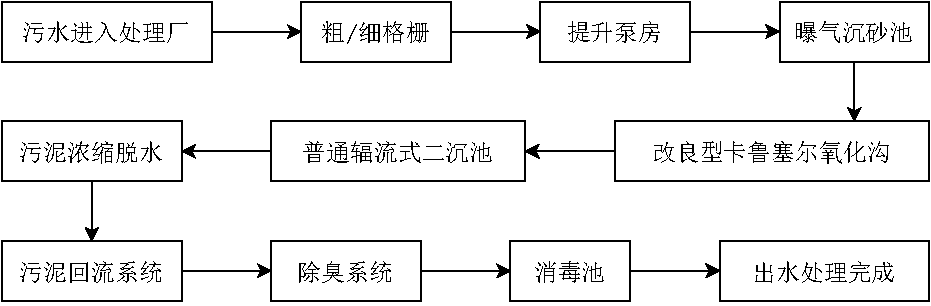
\includegraphics[width=0.92\textwidth]{figures/flowchart.drawio.pdf}
	% \begin{tikzpicture}[node distance=2cm, every node/.style={rectangle, draw, minimum width=3cm, minimum height=1cm, align=center}]
	%     \node (inlet) {污水进入处理厂};
	%     \node (coarse) [right=1.5cm of inlet] {粗格栅};
	%     \node (fine) [right=1.5cm of coarse] {细格栅};
	%     \node (pump) [right=1.5cm of fine] {提升泵房};
	%     \node (aeration) [below=1.5cm of pump] {曝气沉砂池};
	%     \node (oxidation) [left=1.5cm of aeration] {改良型卡鲁塞尔氧化沟};
	%     \node (settling) [left=1.5cm of oxidation] {普通辐流式二沉池};
	%     \node (thickening) [left=1.5cm of settling] {污泥浓缩};
	%     \node (recycle) [below=1.5cm of thickening] {污泥回流系统};
	%     \node (deodorization) [right=1.5cm of recycle] {除臭系统};
	%     \node (disinfection) [right=1.5cm of deodorization] {消毒池};
	%     \node (outlet) [right=1.5cm of disinfection] {出水处理完成};

	%     \draw[->] (inlet) -- (coarse);
	%     \draw[->] (coarse) -- (fine);
	%     \draw[->] (fine) -- (pump);
	%     \draw[->] (aeration) -- (oxidation);
	%     \draw[->] (oxidation) -- (settling);
	%     \draw[->] (recycle) -- (deodorization);
	%     \draw[->] (deodorization) -- (disinfection);
	%     \draw[->] (disinfection) -- (outlet);

	%     % Additional arrows for the S-shape layout
	%     \draw[->] (pump) |- (aeration);
	%     \draw[->] (thickening) |- (recycle);
	% \end{tikzpicture}
	\caption{城镇污水处理厂处理流程图}
	\label{fig:flowchart}
\end{figure}

\subsubsection{进出水质}
根据准备设计的城镇污水处理厂(日平均流量 $Q=35000$ m$^3$/d)的进水水质,我们在制定出水水质要求时优先选择更严格的地方标准,参考《城镇污水处理厂污染物排放标准》A标准(见表 \ref{tab:Pollutant discharge standards for urban sewage treatment plants})以及《四川省岷江、沱江流域水污染物排放标准》城镇污水处理厂污染物排放标准(见表 \ref{tab:Water pollutant discharge standards in the Minjiang and Tuojiang River basins of Sichuan Province})。这样的选择确保了城镇污水处理厂的出水能够满足地方环境保护要求。当地方标准无法明确规定时,我们将参考国家标准来确定出水水质要求。通过这种方法,我们能够确保排放的污水达到最高的环境质量标准,从而有效地保护周围水体和生态环境的健康。
但又考虑到本次城镇污水处理厂的设计地区并不在四川省岷江、沱江流域,综合考虑之下,本次设计会优先满足国家A标准,若是工艺优良,在能力之余则跟进满足地方标准。
以下是具体的进出水水质要求和标准:

\begin{table}[H]
	\centering
	\caption{进出水水质}
	\begin{tabular}{cccc}
		\toprule
		污染物   & 进水水质(mg/L) & 出水水质(mg/L) & 要求去除效率(\%) \\
		\midrule
		COD$\mathrm{_{C_r}}$ & 400   & 50    & 87.5  \\
		BOD$_5$  & 260   & 10     & 96.2 \\
		SS    & 280   & 10    & 96.4  \\
		NH$_4^+$-N\footnotemark & 35    & 5(8) & 85.7  \\
		TP    & 3     & 0.5   & 83.3  \\
		TN    & 45    & 15    & 66.7  \\
		\bottomrule
	\end{tabular}%
	\label{tab:in water}%
\end{table}%
\footnotetext{括号外数值为水温 $>12$ ℃时的控制指标,括号内数值为水温 $\leqslant 12$ ℃时的控制指标。}

\subsection{设计依据}
\subsubsection{法律法规}
\begin{enumerate}
	\item 《水污染防治行动计划》(2015.04);
	\item 《中华人民共和国环境保护法》(2015.01);
	\item 《中华人民共和国水污染防治法》(2008.06)。
\end{enumerate}

\subsubsection{参考规范及标准}
\begin{enumerate}
	\item 《室外排水设计规范》(GB 50014-2021);
	\item 《城镇污水处理厂污染物排放标准》(GB 18918-2002);
	\item 《建筑给水排水设计标准》(GB 50015-2019)
	\item 《四川省岷江、沱江流域水污染物排放标准》(DB 51/2311-2016);
	\item 《氧化沟活性污泥法污水处理工程技术规范》(HJ 578-2010)
	\item 《污水气浮处理工程技术规范》(HJ 2007-2010)
	\item 《给排水制图标准》GB/T50106-2001(2010 年);
	\item 《四川省建设工程工程量清单计价定额市政工程》(2020 年);
	\item 《关于印发城镇污水处理提质增效三年行动方案(2019-2021 年)的通知》。
\end{enumerate}



\newpage % 章节结尾换页 % 设计说明书部分
%============================计算说明书============================%
\Genshinsection{计算说明书}
\section{处理构筑物设计及选型}
\subsection{格栅}
\subsubsection{基础数据}
\begin{enumerate}
	\item 污水平均日流量$Q$:
	$$Q=35000\;\text{m$^3$/d}=35000\times\dfrac{1000}{24\times60\times60}\;\text{L/s}=\eval{35000\times\dfrac{1000}{24\times60\times60}}[3]\;\text{L/s}$$
	\item 生活污水量总变化系数$K_z$:
	
	查阅《室外排水设计标准》(GB 50014-2021)可得到综合生活污水量变化系数表如下:
	\begin{table}[H]
		\centering
		\caption{综合生活污水量变化系数\cite{GB500152019}}
		\begin{tabular}{ccccccccc}
		\toprule
		平均日流量(L/s) & 5     & 15    & 40    & 70    & 100   & 200   & 500   & $\geqslant 1000$ \\
		\midrule
		变化系数  & 2.7   & 2.4   & 2.1   & 2.0     & 1.9   & 1.8   & 1.6   & 1.5 \\
		\bottomrule
		\multicolumn{9}{l}{注:当污水平均日流量为中间数值时,变化系数可用内插法求得。} \\
		\end{tabular}
		\label{tab:Comprehensive domestic sewage volume change coefficient}
	\end{table}

	因为污水平均日流量$Q=405.093\;\text{L/s}$,处于$200\;\text{L/s}\sim 500\;\text{L/s}$之间,则可以使用内插法求得:

	\begin{equation}
		\dfrac{Q-200}{K_z-1.8}=\dfrac{500-200}{1.6-1.8}
	\end{equation}
	\begin{align*}
		\therefore K_z=\dfrac{1.6-1.8}{500-200}(Q-200)+1.8 &=\dfrac{1.6-1.8}{500-200}\times(405.093-200)+1.8 \\
		&=\eval{\dfrac{1.6-1.8}{500-200}\times(405.093-200)+1.8}[2]
	\end{align*}

	\item 设计最大流量$Q_{max}$:
	$$Q_{max}=K_zQ=\workKz\times 35000\;\text{m$^3$/d}=58100 \;\text{m$^3$/d}=\eval{35000\times\dfrac{1}{24\times60\times60}\times1.66}[3]\;\text{m$^3$/s}$$
\end{enumerate}

\subsubsection{粗格栅计算草图}
粗格栅的主要功能是通过物理筛选的方式将污水中的大块固体物质、悬浮物、杂草、沙子等较大的颗粒物拦截下来,以防止它们进入后续的处理单元,从而减少对系统的损坏和故障的影响。

% 本次设计粗格栅由一组格栅宽度为 193 mm 的金属栅条与金属框架组成,其中栅条宽度为 $S=10$ mm,进水渠宽 $B_1=1.26$ m,格栅与水平面夹角 $\alpha$ 为60°,如下图所示:

\vskip2em

\begin{figure}[H]
	\centering
	% 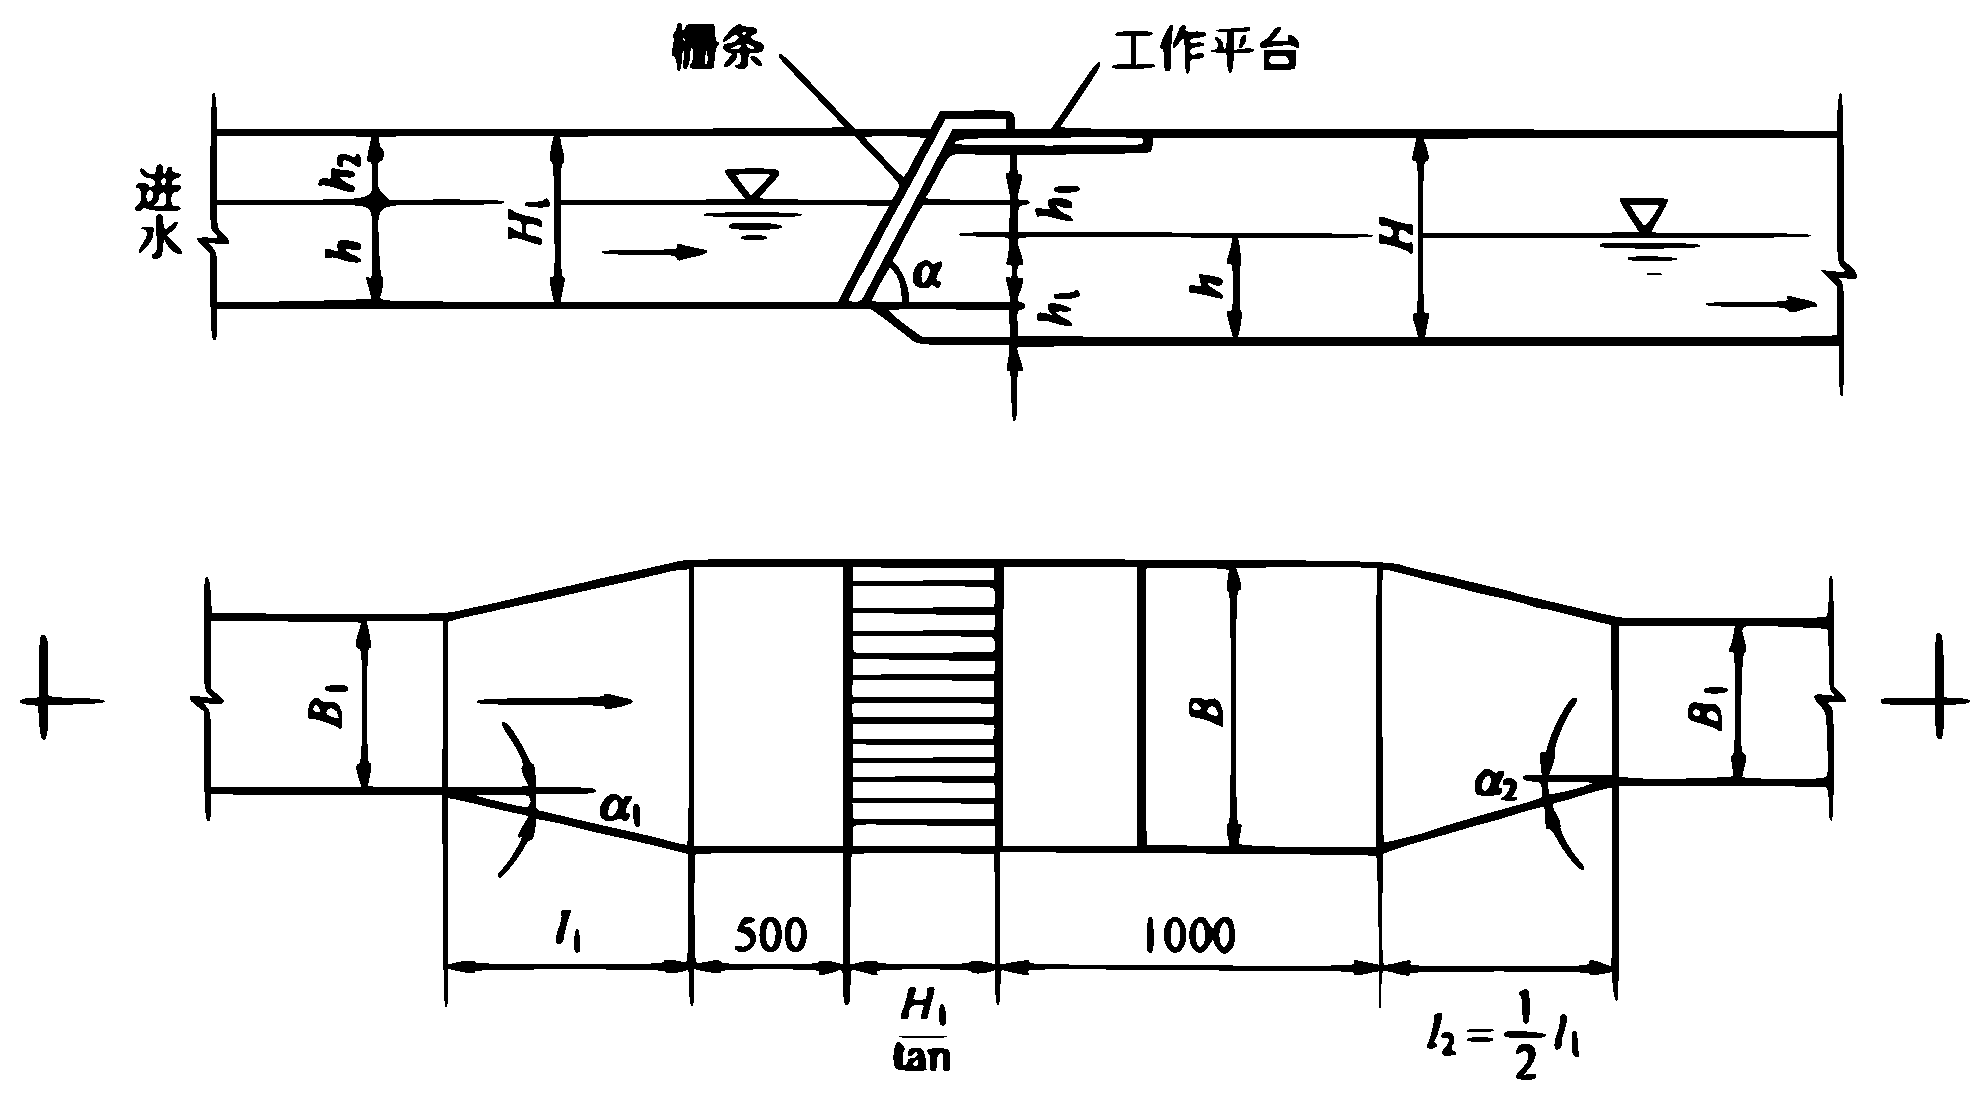
\includegraphics[width=\textwidth]{figures/Coarse-grille-sketch.pdf}
	\begin{subfigure}[htbp]{\textwidth}
		\centering
		\begin{tikzpicture}[scale=0.8]
			% 画折断线
			\draw (0,-0.5) -- ++(0,1) -- ++(-0.2,0.2) -- ++(0.4,0) -- ++(-0.2,0.2) -- (0,2.5);
			\draw (16,-1) -- ++(0,1) -- ++(-0.2,0.2) -- ++(0.4,0) -- ++(-0.2,0.2) -- (16,2.5);
			\node[left] at (-0.3,1) {进水};
			\node[right] at (16.3,1) {\phantom{进水}};
			% 画主体
			\draw (0,2) -- ++(16cm,0);
			\draw (0,1.2) -- ++(8cm,0);
			\draw (7.5,0.7) -- (16,0.7);
			\draw (0,0) -- ++(8cm,0);
			\draw (16,-0.5) -- ++(-9cm,0) -- ++(-0.5,0.5);
			% 画工作平台
			\draw (8,2) -- ++(2,0) -- ++(0,-0.2) -- ++(-2,0) -- cycle;
			\draw (8.8,2) -- ++(1,1) node[right] {工作平台};
			% 标记符号
			\draw (6.3,0) ++(0.5,0) arc (0:60:0.5) node[midway, right] {$\alpha$};
			\draw[stealth-stealth] (1.5,0) -- (1.5,1.2) node[midway, left] {$h$};
			\draw[stealth-stealth] (1.5,1.2) -- (1.5,2) node[midway, left] {$h_2$};
			\draw[stealth-stealth] (3,0) -- (3,2) node[midway, below left] {$H_1$};
			\draw[stealth-stealth] (8,-0.5) -- ++(0,0.5) node[right] {$h_1$};
			\draw[stealth-stealth] (8,0.7) -- ++(0,0.5) node[right] {$h_1$};
			\draw[stealth-stealth] (10,-0.5) -- ++(0,1.2) node[midway, left] {$h$};
			\draw[stealth-stealth] (12,-0.5) -- ++(0,2.5) node[midway, above left] {$H$};
			% 画格栅
			\draw (7.4,1.5) -- ++(-1.5,1.5) node[left] {格栅};
			\draw[fill=white] (8,2) -- ++(0.6,0) -- ++(0,0.15) -- ++(-0.65,0) -- (6,0) -- ++(0.2,0) -- cycle;
			% 画标识
			\draw[-stealth, line width=1.2pt] (3.5,0.6) -- ++(1,0);
			\draw[-stealth, line width=1.2pt] (14.5,0.1) -- ++(1,0);
			\foreach \x/\y in {5/1.2, 14/0.7} {
				\draw (\x,\y) -- ++(-0.3,0.3) -- ++(0.6,0) --cycle;
				\draw (\x,\y) ++(-0.5,-0.1) -- ++(1,0);
				\draw (\x,\y) ++(-0.3,-0.2) -- ++(0.6,0);
				\draw (\x,\y) ++(-0.1,-0.3) -- ++(0.2,0);
			}
		\end{tikzpicture}
		\caption{正视图}
	\end{subfigure}

	\begin{subfigure}[htbp]{\textwidth}
		\centering
		\begin{tikzpicture}[scale=0.8]
			% 画对称线
			\draw (-2,1) ++(-0.5,0) -- ++(1.5,0);
			\draw (-2,1) ++(0,-0.5) -- ++(0,1.5);
			\draw (18,1) ++(-1,0) -- ++(1.5,0);
			\draw (18,1) ++(0,-0.5) -- ++(0,1.5);
			% 画折断线
			\draw (0,-0.5) -- ++(0,1.3) -- ++(-0.2,0.2) -- ++(0.4,0) -- ++(-0.2,0.2) -- (0,2.5);
			\draw (16,-0.5) -- ++(0,1.3) -- ++(-0.2,0.2) -- ++(0.4,0) -- ++(-0.2,0.2) -- (16,2.5);
			% 画主体
			\foreach \d in {0.6} {
				\draw (0,0) -- ++(1.5,0) -- ++(2.5,-\d)-- ++(8,0) -- ++(2.5,\d) -- ++(1.5,0);
				\draw (0,2) -- ++(1.5,0) -- ++(2.5,\d)-- ++(8,0) -- ++(2.5,-\d) -- ++(1.5,0);
				\foreach \x in {1.5,14.5} {
					\draw (\x,0) -- ++(0,2);
				}
				\foreach \x in {4,6,8,9.5,12} {
					\draw (\x,-\d) -- ++(0,2+2*\d);
				}
				\foreach \y in {0,0.1,...,1} {
					\draw (6,{\y*(2+2*\d)-\d}) -- ++(2,0);
				}
				% 画标注
				\foreach \y in {1.2} {
					\draw (1.5,0) -- ++(0,-\y-\d);
					\draw (14.5,0) -- ++(0,-\y-\d);
					\foreach \x in {4,6,8,12} {
						\draw (\x,-\d) -- ++(0,-\y);
					}
					\draw[stealth-stealth] (1.5,0.2-\y-\d) -- ++(2.5,0) node[midway, above] {$l_1$};
					\draw[stealth-stealth] (14.5,0.2-\y-\d) -- ++(-2.5,0) node[midway, below] {$l_2=\dfrac{1}{2}l_1$};
					\draw[stealth-stealth] (4,0.2-\y-\d) -- ++(2,0) node[midway, above] {$500$};
					\draw[stealth-stealth] (6,0.2-\y-\d) -- ++(2,0) node[midway, below] {$\dfrac{H_1}{\tan{\alpha}}$};
					\draw[stealth-stealth] (8,0.2-\y-\d) -- ++(4,0) node[midway, above] {$1000$};
				}
				\foreach \x in {1,15.5} {
					\draw[stealth-stealth] (\x,0) -- ++(0,2) node[midway, left] {$B_1$};
				}
				\draw[stealth-stealth] (10.5,-\d) -- ++(0,{2+2*\d}) node[midway, left] {$B$};
				\draw[-stealth, line width=1.2pt] (2,1) -- ++(1.5,0);
				% 画角度
				\draw (3.5,0) -- ++(-2,0) ++(1.5,0) arc (0:-{atan(\d/2.5)}:1.5cm) node[midway, right] {$\alpha_1$};
				\draw (12.5,0) -- ++(2,0) ++(-1.5,0) arc (180:{180+atan(\d/2.5)}:1.5cm) node[midway, left] {$\alpha_2$};
			}
		\end{tikzpicture}
		\caption{俯视图}
	\end{subfigure}

	\caption{粗格栅计算草图}
	\label{fig:Coarse grille sketch}
\end{figure}


\subsubsection{粗格栅的计算}
一般格栅的计算理论主要是以平面格栅为研究对象,对于曲面格栅应考虑折减和换算。在进行工程设计和格栅选型时,应在格栅理论计算的基础上,结合工程设计实际和选型格栅特点统筹考虑。查阅张辰主编的《污水厂设计》得到格栅设计相关计算公式如下:

\footnotesize
\begin{longtable}{l|l|l}
	\caption{格栅设计计算公式\cite[p.114]{《污水厂设计》}}\label{tab:Grille design calculation formula} \\
	\toprule
	名称    & 公式    & 符号说明 \\
	\midrule
	\endfirsthead
	
	\multicolumn{3}{c}%
	{{\tablename\ \thetable{} -- 续表}} \\
	\toprule
	名称    & 公式    & 符号说明 \\
	\midrule
	\endhead
	
	\bottomrule
	\endfoot
	
	\bottomrule
	\endlastfoot
	
	栅槽宽度 & \makecell[l]{$B=S(n-1)+bn+0.2$\\ $n =\dfrac{Q_{max}\sqrt{\sin\alpha}}{bhv}$} & \makecell[l]{$B$——栅槽宽度,m;\\
	$S$——栅条宽度,m;\\
	$b$——栅条间隙,m;\\
	$n$——栅条间隙数,个;\\
	$Q_{max}$——最大设计流量,m$^3$/s;\\
	$\alpha$——格栅倾角,度;\\
	$h$——栅前水深,m;\\
	$v$——过栅流速,m/s} \\
	
	\midrule
	通过格栅的水头损失 & \makecell[l]{$h_1=h_0k$\\ $h_0=\xi\dfrac{v^2}{2g}\sin\alpha$} & \makecell[l]{$h_1$——通过格栅的水头损失,m;\\
	$h_0$——计算水头损失,m;\\
	$g$——重力加速度,m/s$^2$;\\
	$k$——系数,格栅受污物堵塞时水头损失增大倍数,\\
	\phantom{$k$——}一般采用3;\\
	$\xi$——阻力系数,其值与栅条断面形状有关,\\
	\phantom{$\xi$——}可按表 \ref{tab:The drag coefficient xi calculation formula} 计算} \\
	
	\midrule
	栅后槽总高度  & $H=h+h_1+h_2$   & \makecell[l]{$H$——栅后槽总高度,m;\\
	$h_2$——栅前渠道超高,一般采用 0.3 m} \\
	
	\midrule
	栅槽总长度  &  \makecell[l]{$L=l_1+l_2+1.0+0.5+\dfrac{H_1}{\tan\alpha}$\\ $l_1=\dfrac{B-B_1}{2\tan\alpha_1}$\\ $l_2=\dfrac{l_1}{2}$\\ $H_1=h+h_2$}   & \makecell[l]{$L$——栅槽总长度,m;\\
	$l_1$——进水渠道渐宽部分的长度,m;\\
	$B_1$——进水渠宽,m;\\
	$\alpha_1$——进水渠道渐宽部分的展开角度,一般可采用20°;\\
	$l_2$——栅渣与出水渠道连接处的渐窄部分长度,m;\\
	$H_1$——栅前渠道深,m} \\
	
	\midrule
	每日栅渣量 & \makecell[l]{$W=\dfrac{Q_{max}W_1\times86400}{K_z\times1000}$} &  \makecell[l]{$W$——每日栅渣量,m$^3$/d;\\
	$W_1$——单位栅渣量,m$^3$/10$^3$m$^3$ 污水;\\
	格栅间隙为 $16\sim 25$ mm时,$W_1=0.10\sim 0.05$;\\
	格栅间隙为 $30\sim 50$ mm时,$W_1=0.03\sim 0.01$;\\
	$K_z$——生活污水流量总变化系数} \\
\end{longtable}
\normalsize

\begin{table}[H]
	\centering
	\caption{阻力系数 $\xi$ 计算公式\cite[p.114]{《污水厂设计》}}
	\begin{tabular}{l|l|l}
		\toprule
		棚条断面形状    & 公式    & 说明 \\
		\midrule
		\makecell[l]{\null\\锐边矩形\\迎水面为半圆形的矩形\\圆形\\迎水、背水面均为半圆形的矩形} & $\xi=\beta\left(\dfrac{S}{b}\right)^{\frac{4}{3}}$ & \makecell[l]{形状系数\\ $\beta=2.42$\\ $\beta=1.83$\\ $\beta=1.79$\\ $\beta=1.67$} \\
		\midrule
		正方形 & $\xi=\left(\dfrac{b+S}{\varepsilon b}-1\right)^{2}$ & \makecell[l]{$\varepsilon$——收缩系数,一般采用0.64} \\
		\bottomrule
	\end{tabular}%
	\label{tab:The drag coefficient xi calculation formula}%
\end{table}%


\begin{enumerate}
	\item 栅槽宽度
	
	\begin{enumerate}
		\item 栅前水深、进水渠宽:
		
		水力最优梯形断面宽深比\cite{水力最优——《水力学》第六章}:
		\begin{equation}
			\beta = \dfrac{b}{h} =2\left(\sqrt{1+m^2}-m\right)
		\end{equation}
		$b$——进水渠宽,m;\par
		$h$——栅前水深,m;\par
		$m$——边坡系数。
		
		因为进水渠形状设计为矩形,如下图 \ref{fig:Sketch of the shape of the intake canal} 所示:
		\begin{figure}[H]
			\centering
			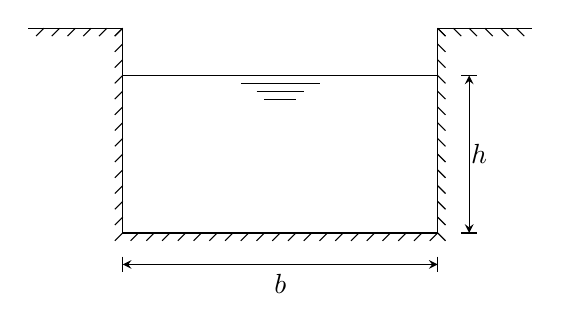
\begin{tikzpicture}
				\draw (-1.2,2.6) -- (0,2.6) -- (0,0) -- (4,0) -- (4,2.6) -- (5.2,2.6);
				\foreach \x in {0,0.2,...,4} % 绘制地面上的刻度线
					\draw (\x,0) -- (\x-0.1,-0.1);
				\foreach \x in {-1,-0.8,...,0} % 绘制地面上的刻度线
					\draw (\x,2.6) -- (\x-0.1,2.5);
				\foreach \x in {4,4.2,...,5} % 绘制地面上的刻度线
					\draw (\x,2.6) -- (\x+0.1,2.5);
				\foreach \y in {0.2,0.4,...,2.6} % 绘制地面上的刻度线
					\draw (0,\y) -- (-0.1,\y-0.1);
				\foreach \y in {0,0.2,...,2.6} % 绘制地面上的刻度线
					\draw (4,\y) -- (4.1,\y-0.1);

				\draw (0,2) -- (4,2); % 水面高度
				\draw (2,2) ++(-0.5,-0.1) -- ++(1,0);
				\draw (2,2) ++(-0.3,-0.2) -- ++(0.6,0);
				\draw (2,2) ++(-0.2,-0.3) -- ++(0.4,0);
			
				\foreach \x in {0,2}
					\draw (4.3,\x) -- (4.5,\x);
				\draw[stealth-stealth] (4.4,0) -- (4.4,2);
				\node[right] at (4.3,1) {$h$};
				\foreach \x in {0,4}
					\draw (\x,-0.3) -- (\x,-0.5);
				\draw[stealth-stealth] (0,-0.4) -- (4,-0.4);
				\node[below] at (2,-0.4) {$b$};
			\end{tikzpicture}
			\caption{进水渠形状草图}
			\label{fig:Sketch of the shape of the intake canal}
		\end{figure}
		则易知边坡系数 $m=0$ ,所以
		\begin{equation*}
			\beta = \dfrac{b}{h} =2\left(\sqrt{1+0^2}-0\right) = 2
		\end{equation*}
		即
		\begin{equation}
			b=2h
		\end{equation}

		明渠均匀流基本公式\cite{水力最优——《水力学》第六章}:
		\begin{equation}
			Q=Av
		\end{equation}
		$Q$——流量,m$^3$;\par
		$A$——截面面积,m$^2$;\par
		$v$——流速,m/s。取 $v=0.85$ m/s\footnote{《室外排水设计标准》(GB 50014-2021):污水过栅流速宜采用 0.6 m/s $\sim$ 1.0 m/s。}。

		又因为进水渠的截面面积为
		\begin{equation}
			A=bh
		\end{equation}

		所以当流量为设计最大流量 $Q_{max}=0.672$ m$^3$/s 时,将上述公式联立求解,可得到每台格栅机栅前水深 $h$、进水渠宽 $B_1$:
		\begin{align*}
			B_1=b=\sqrt{\dfrac{2Q_{max}}{v}}=\sqrt{\dfrac{2\times0.672}{0.85\times2}} \;\text{m} =\eval{\sqrt{\dfrac{2\times0.672}{0.85\times2}}}[2] \;\text{m} \\
			h=h=\sqrt{\dfrac{Q_{max}}{2v}}=\sqrt{\dfrac{0.672}{2\times 0.85\times2}} \;\text{m} = \eval{\sqrt{\dfrac{0.672}{2\times 0.85\times2}}}[2] \;\text{m}
		\end{align*}
		\item 栅条的间隙数:
		
		因为格栅选择的是机械清除,所以取 $b=0.021$ m\footnote{《室外排水设计标准》(GB 50014-2021)粗格栅栅条间隙宽度规定:机械清除时宜为16 mm $\sim$ 25 mm,人工清除时宜为25 mm $\sim$ 40 mm,特殊情况下,最大间隙可为100 mm。},
		取 $\alpha=60$°\footnote{《室外排水设计标准》(GB 50014-2021):除转鼓式格栅除污机外,机械清除格栅的安装角度宜为 60°$\sim$90°。},
		共有2台格栅机器,则每台格栅机器的栅槽宽度为
		\begin{align}
			n =\dfrac{Q_{max}\sqrt{\sin\alpha}}{bhv}&=\dfrac{\dfrac{0.672}{2}\times\sqrt{\sin{\dfrac{\pi}{3}}}}{0.021\times0.44\times0.85}=\eval{\dfrac{\frac{0.672}{2}\times\sqrt{\sin{\frac{\pi}{3}}}}{0.021\times0.44\times0.85}}[1] \;\text{(条)}\\
			&\approx 40\;\text{(条,向上取整)} \notag
		\end{align}
		
		\item 栅槽宽度:

		因为栅条宽度 $S=0.01$ m,则
		\begin{align}
			B=S(n-1)+bn+0.2 &=0.01\times(40-1)+0.021\times40+0.2 \;\text{m} \\
			&=\eval{0.01\times(40\times 2-1)+0.021\times40+0.2}[2]\;\text{m} \notag
		\end{align}
	\end{enumerate}
	
	\item 通过格栅的水头损失
	
	\begin{enumerate}
		\item 计算水头损失:

		因为栅条断面形状为锐边矩形,由表 \ref{tab:The drag coefficient xi calculation formula} 可知$\beta=2.42$,则
		\begin{align}
			\xi=\beta\left(\dfrac{S}{b}\right)^{\frac{4}{3}} =2.42\times\left(\dfrac{0.01}{0.021}\right)^{\frac{4}{3}}=\eval{2.42\times\left(\dfrac{0.01}{0.021}\right)^{\frac{4}{3}}}[3] 
		\end{align}

		又因为重力加速度 $g=9.8$ m/s$^2$,则
		\begin{align}
			h_0=\xi\dfrac{v^2}{2g}\sin\alpha=0.9\times\dfrac{0.85^2}{2\times9.8}\sin{\frac{\pi}{3}}\;\text{m}=\eval{0.9\times\dfrac{0.85^2}{2\times9.8}\sin{\frac{\pi}{3}}}[4] \;\text{m}
		\end{align}

		\item 通过格栅的水头损失:

		取 $k=3$\footnote{由表 \ref{tab:Grille design calculation formula} 可知,系数 $k$,格栅受污物堵塞时水头损失增大倍数,一般采用3。},则
		\begin{align}
			h_1=h_0k=0.0287\times3 \;\text{m}=\eval{0.9\times\dfrac{0.85^2}{2\times9.8}\sin{\frac{\pi}{3}}\times3}[3]\;\text{m}
		\end{align}
	\end{enumerate}
	
	\item 栅后槽总高度
	
	取 $h_2=0.3$ m\footnote{由表 \ref{tab:Grille design calculation formula} 可知,栅前渠道超高一般采用 0.3 m。},	则
	\begin{align}
		H=h+h_1+h_2=0.44+0.086+0.3\;\text{m}=\eval{0.44+0.086+0.3}\;\text{m}
	\end{align}
	\item 栅槽总长度
	
	\begin{enumerate}
		\item 栅前渠道深:
		\begin{equation}
			H_1=h+h_2=0.44+0.3\;\text{m}=0.74\;\text{m}
		\end{equation}
		\item 进水渠道渐宽部分的长度:
		
		取 $\alpha_1=20$°\footnote{由表 \ref{tab:Grille design calculation formula} 可知,进水渠道渐宽部分的展开角度,一般可采用20°。},则
		\begin{equation}
			l_1=\dfrac{B-B_1}{2\tan\alpha_1}=\dfrac{1.83-0.89}{2\tan{20}\text{°}}\;\text{m}=\eval{\dfrac{1.83-0.89}{2\tan{20/180*\pi}}}[2]\;\text{m}
		\end{equation}

		\item 栅渣与出水渠道连接处的渐窄部分长度:
		\begin{equation}
			l_2=\dfrac{l_1}{2}=\dfrac{1.29}{2}\;\text{m}=\eval{\dfrac{1.29}{2}}\;\text{m}
		\end{equation}

		\item 栅槽总长度:
		\begin{align}
			L=l_1+l_2+1.0+0.5+\dfrac{H_1}{\tan\alpha}&=1.29+0.645+1.0+0.5+\dfrac{0.74}{\tan{60}\text{°}}\;\text{m}\\
			&=\eval{1.29+0.645+1.0+0.5+\dfrac{0.74}{\tan{60/180*\pi}}}[2]\;\text{m} \notag
		\end{align}
	\end{enumerate}
	
	\item 每日栅渣量

	取 $W_1=0.07$ m$^3$/10$^3$m$^3$\footnote{由表 \ref{tab:Grille design calculation formula} 可知,格栅间隙 $b=21$ mm 为 $16\sim 25$ mm时,单位栅渣量 $W_1=0.10\sim 0.05$ m$^3$/10$^3$m$^3$。则$\dfrac{0.10-0.05}{16-25}=\dfrac{W_1-0.05}{b-25}$,$W_1=\dfrac{0.10-0.05}{16-25}\times(b-25)+0.05 =\dfrac{0.10-0.05}{16-25}\times(21-25)+0.05 \;\text{m$^3$/10$^3$m$^3$} =\eval{\dfrac{0.10-0.05}{16-25}\times(21-25)+0.05}[2] \;\text{m$^3$/10$^3$m$^3$}$。},共有 2 台格栅机器,则每台每日栅渣量为
	\begin{align}
		W=\dfrac{Q_{max}W_1\times86400}{K_z\times1000}&=\dfrac{\dfrac{0.672}{2}\times0.07\times86400}{1.66\times1000}\;\text{m$^3$/d} \\
		&=\eval{\dfrac{\dfrac{0.672}{2}\times0.07\times86400}{1.66\times1000}}[3]\;\text{m$^3$/d}  \notag \\
		&> 0.2 \;\text{m$^3$/d(符合机械清渣要求)}  \notag
	\end{align}
\end{enumerate}


\subsubsection{细格栅设计数据}

细格栅广泛应用于污水处理系统的初级阶段,用于有效去除污水中的固体悬浮物和大颗粒物质。其主要目的是防止这些大颗粒物质进入后续处理单元,以保护设备的正常运行,并减轻后续处理单元的负荷。细格栅与粗格栅在设计上有相似之处,但最本质的区别在于两者格栅栅条间隙宽度的不同。因此,除非特殊要求,可以采用粗格栅的计算公式进行细格栅的设计计算(参见表 \ref{tab:Grille design calculation formula})。根据中华人民共和国住房和城乡建设部《室外排水设计标准》(GB 50014-2021)规定,细格栅的格栅栅条间隙宽度宜在1.5 mm $\sim$ 10 mm之间。在此情况下,我们选择了 $b=6.0$ mm作为间隙宽度,并保持其他数据取值不变。


根据粗格栅水力最优梯形断面公式和明渠均匀流基本公式,联立可得到栅前水深 $h$、进水渠宽 $B_1$:
\begin{align*}
	B_1=b=\sqrt{\dfrac{2Q_{max}}{v}}=\sqrt{\dfrac{2\times0.672}{0.85\times2}} \;\text{m} =\eval{\sqrt{\dfrac{2\times0.672}{0.85\times2}}}[2] \;\text{m} \\
	h=h=\sqrt{\dfrac{Q_{max}}{2v}}=\sqrt{\dfrac{0.672}{2\times 0.85\times2}} \;\text{m} = \eval{\sqrt{\dfrac{0.672}{2\times 0.85\times2}}}[2] \;\text{m}
\end{align*}
将细格栅设计基础数据汇总,具体取值如下表 \ref{tab:Fine grille design basic data} 所示:
\begin{table}[H]
  \centering
  \caption{细格栅设计基础数据}
    \begin{tabular}{p{0.45\textwidth}*{3}{p{0.08\textwidth}}}
    \toprule
    数据    & 符号    & 值     & 单位 \\
    \midrule
    设计流量  & $Q$     & 35000 & m$^3$/d \\
    综合生活污水量变化系数 & $K_z$    & 1.66  &  \\
    最大设计流量 & $Q_{max}$  & 58100 & m$^3$/d \\
    \midrule
	栅前水深  & $h$     & 0.44 & m \\
	进水渠宽  & $B_1$     & 0.89 & m \\
    细格栅机数量 &       & 2     & 台 \\
	\midrule
    栅条间隙  & $b$     & 0.006 & m \\
    格栅倾角  & $\alpha$ & 60    & ° \\
    栅条宽度  & $S$     & 0.01  & m \\
    过栅流速  & $v$     & 0.85  & m/s \\
	\midrule
    棚条断面形状(锐边矩形)形状系数 & $\beta$  & 2.42  &  \\
    重力加速度 & $g$     & 9.8   & m/s$^2$ \\
    格栅受污物堵塞时水头损失增大倍数 & $k$     & 3     &  \\
    栅前渠道超高 & $h_2$    & 0.3   & m \\
    进水渠道渐宽部分的展开角度 & $\alpha_1$ & 20    & ° \\
    \bottomrule
    \end{tabular}%
  \label{tab:Fine grille design basic data}%
\end{table}%


\subsubsection{细格栅的计算}

\begin{enumerate}
	\item 栅槽宽度
	\begin{enumerate}
		\item 栅条的间隙数:
		
		每台格栅机器的栅槽宽度为
		\begin{align}
			n =\dfrac{Q_{max}\sqrt{\sin\alpha}}{bhv}&=\dfrac{\dfrac{58100}{2\times 86400}\times\sqrt{\sin{\dfrac{\pi}{3}}}}{0.006\times0.44\times0.85}=\eval{\dfrac{\dfrac{58100}{2\times 86400}\times\sqrt{\sin{\frac{\pi}{3}}}}{0.006\times0.44\times0.85}}[2] \;\text{(条)}\\
			&\approx 140\;\text{(条,向上取整)} \notag
		\end{align}
		
		\item 栅槽宽度:

		因为格栅机器台数为2,则
		\begin{align}
			B=S(n-1)+bn+0.2 &=0.01\times(140-1)+0.006\times140+0.2 \;\text{m} \\
			&=\eval{0.01\times(140-1)+0.006\times140+0.2}[2]\;\text{m} \notag
		\end{align}
	\end{enumerate}
	
	\item 通过格栅的水头损失
	
	\begin{enumerate}
		\item 计算水头损失:

		\begin{align}
			h_0=\xi\dfrac{v^2}{2g}\sin\alpha &= \beta\left(\dfrac{S}{b}\right)^{\frac{4}{3}}\cdot\dfrac{v^2}{2g}\sin\alpha \\
		&=2.42\times\left(\dfrac{0.01}{0.006}\right)^{\frac{4}{3}}\times\dfrac{0.85^2}{2\times9.8}\sin{\frac{\pi}{3}}\;\text{m} \notag \\
		&=\eval{2.42\times\left(\dfrac{0.01}{0.006}\right)^{\frac{4}{3}}\times\dfrac{0.85^2}{2\times9.8}\sin{\frac{\pi}{3}}}[4] \;\text{m} \notag
		\end{align}

		\item 通过格栅的水头损失:

		\begin{align}
			h_1=h_0k=0.1527\times3 \;\text{m}=\eval{4.782\times\dfrac{0.85^2}{2\times9.8}\sin{\frac{\pi}{3}}\times3}[3]\;\text{m}
		\end{align}
	\end{enumerate}
	
	\item 栅后槽总高度
	
	\begin{align}
		H=h+h_1+h_2=0.44+0.458+0.3\;\text{m}=\eval{0.44+0.458+0.3}\;\text{m}
	\end{align}
	\item 栅槽总长度
	
	\begin{enumerate}
		\item 栅前渠道深:
		\begin{equation}
			H_1=h+h_2=0.44+0.3\;\text{m}=0.73\;\text{m}
		\end{equation}
		\item 进水渠道渐宽部分的长度:
		
		\begin{equation}
			l_1=\dfrac{B-B_1}{2\tan\alpha_1}=\dfrac{2.43-0.89}{2\tan{20}\text{°}}\;\text{m}=\eval{\dfrac{2.43-0.89}{2\tan{20/180*\pi}}}[2]\;\text{m}
		\end{equation}

		\item 栅渣与出水渠道连接处的渐窄部分长度:
		\begin{equation}
			l_2=\dfrac{l_1}{2}=\dfrac{2.12}{2}\;\text{m}=\eval{\dfrac{2.12}{2}}\;\text{m}
		\end{equation}

		\item 栅槽总长度:
		\begin{align}
			L=l_1+l_2+1.0+0.5+\dfrac{H_1}{\tan\alpha}&=2.12+1.06+1.0+0.5+\dfrac{0.73}{\tan{60}\text{°}}\;\text{m}\\
			&=\eval{2.12+1.06+1.0+0.5+\dfrac{0.73}{\tan{60/180*\pi}}}[2]\;\text{m} \notag
		\end{align}
	\end{enumerate}
	
	\item 每日栅渣量

	取 $W_1=0.05$ m$^3$/10$^3$m$^3$\footnote{由表 \ref{tab:Grille design calculation formula} 可知,粗格栅间隙 $b=21$ mm 在 $16\sim 25$ mm之间时,单位栅渣量 $W_1=0.10\sim 0.05$ m$^3$/10$^3$m$^3$,取的 $W_1=0.07$ m$^3$/10$^3$m$^3$;又考虑到粗格栅已经对污水进行了初次处理,则细格栅的单位栅渣量取 $W_1=0.05$ m$^3$/10$^3$m$^3$。},共有 2 台格栅机器,则每台每日栅渣量为
	\begin{align}
		W=\dfrac{Q_{max}W_1\times86400}{K_z\times1000}&=\dfrac{\dfrac{0.672}{2}\times0.05\times86400}{1.66\times1000}\;\text{m$^3$/d} \\
		&=\eval{\dfrac{\dfrac{0.672}{2}\times0.05\times86400}{1.66\times1000}}[3]\;\text{m$^3$/d}  \notag \\
		&> 0.2 \;\text{m$^3$/d(符合机械清渣要求)}  \notag
	\end{align}
\end{enumerate}

 % 格栅设计部分
\subsection{沉砂池}
\subsubsection{沉砂池的选择}
在这次处理含有高浓度有机物质的污水的沉砂池设计中(详见表 \ref{tab:in water}),传统的平流沉砂池和竖流沉砂池效果不佳,无法有效去除这些有机物质,增加了后续处理的困难。相比之下,曝气沉砂池结合曝气和沉砂的特点,具有多个优势。它引入气体曝气系统,提供溶解氧,促进微生物生长和活性,加快有机物的降解速率。即使有机物含量高,曝气沉砂池也能更有效地降解它们。此外,曝气沉砂池能够更好地实现悬浮物固液分离,通过增加悬浮物的浮力,使其更容易上升到水面形成浮泡,从而减少悬浮物含量,改善处理效果。此外,曝气沉砂池对处理面积需求小且能耗低。相比传统的平流沉砂池和竖流沉砂池,在相同处理效果下,曝气沉砂池占地面积更小,适用于城镇污水处理厂设计。同时,曝气设备的能耗较低,降低了运行成本。综上,我们选择了曝气沉砂池。\cite[pp.75-87]{《污水处理厂工艺设计手册》}


\subsubsection{曝气沉砂池的计算}
查阅张辰主编的《污水厂设计》,曝气沉砂池设计计算公式如下表 \ref{tab:Aeration grit tank design calculation formula} 所示:
\begin{table}[H]
	\centering
	\caption{曝气沉砂池设计计算公式\cite[p.161]{《污水厂设计》}}
	\begin{tabular}{l|l|l}
		\toprule
		名称    & 公式    & 符号说明 \\
		\midrule
		水池总有效容积 & $V=Q_{max}t\times60$ & \makecell[l]{$V$——水池总有效容积,m$^3$;\\ $Q_{max}$——最大设计流量,m$^3$/s;\\ $t$——最大设计流量时的流行时间,min} \\
		\midrule
		水流断面积 & $A =\dfrac{Q_{max}}{v_1}$ & \makecell[l]{$A$——水流断面积,m$^2$;\\$v_1$——最大设计流量时的水平流速,m/s,\\\phantom{$v_1$——}一般采用 $0.06\sim0.12$ m/s} \\
		\midrule
		池总宽度  & $B=\dfrac{A}{h_2}$   & \makecell[l]{$B$——池总宽度,m;\\$h_2$——设计有效水深,m} \\
		\midrule
		池长    & $L=\dfrac{V}{A}$   & $L$——池长,m \\
		\midrule
		每小时所需空气量 & $q=dQ_{max}\times3600$ &  \makecell[l]{$q$——每小时所需空气量,m$^3$/h;\\$d$——每立方米污水所需空气量(m$^3$/m$^3$)} \\
		\bottomrule
	\end{tabular}%
	\label{tab:Aeration grit tank design calculation formula}%
\end{table}%

\begin{figure}[H]
	\centering
	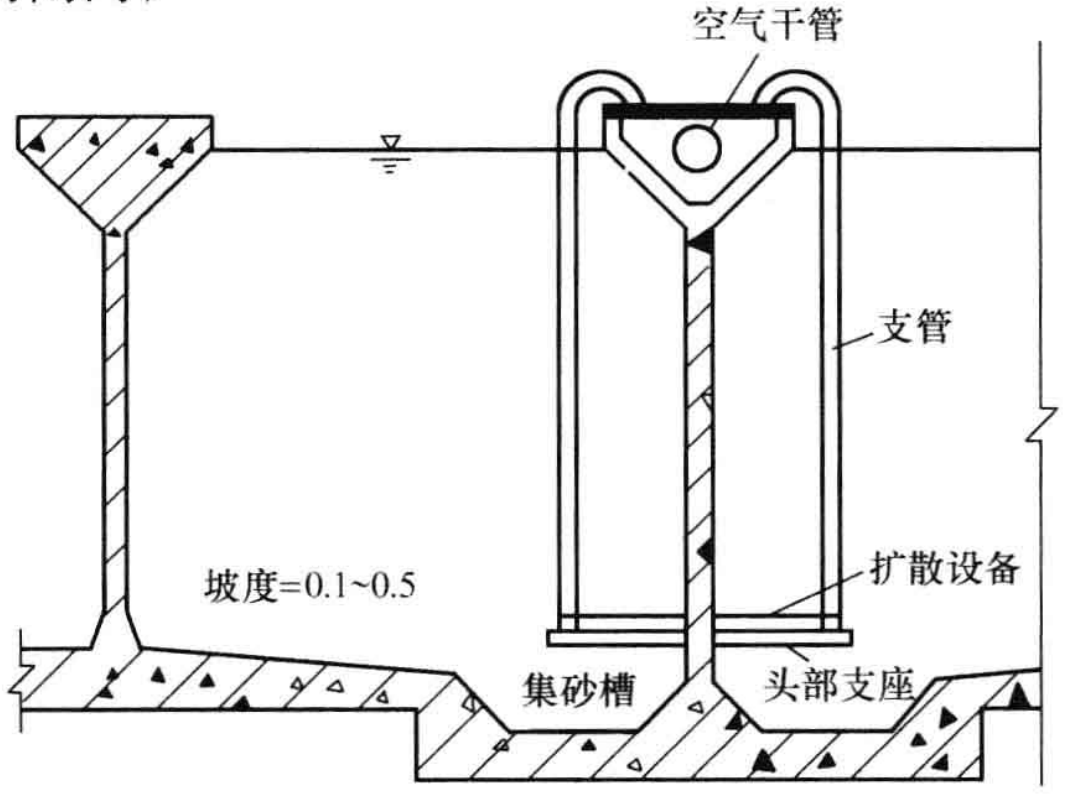
\includegraphics[width=0.6\textwidth]{figures/Sketch of the appearance of the aeration grit tank.png}
	\caption{曝气沉砂池外型草图}
	\label{fig:Sketch of the appearance of the aeration grit tank}
\end{figure}

\begin{enumerate}
	\item 池子总有效容积
	
	设 $t=2$ min\footnote{最大流量时停留时间为 $1\sim3$ min。\cite[p.30]{《城市污水厂处理设施设计计算(第三版)》}},因为曝气沉淀池的个数为2,所以单个曝气沉淀池的总有效容积为:
	\begin{align}
		V=Q_{max}t\times60 =\dfrac{0.672}{2}\times2\times60\;\text{m$^3$} =\eval{\dfrac{0.672}{2}\times2\times60}[3]\;\text{m$^3$}
	\end{align}
	
	\item 水流断面面积

	设$v_1=0.06$ m/s\footnote{由表 \ref{tab:Aeration grit tank design calculation formula} 可知,最大设计流量时的水平流速$v_1$,一般采用 $0.06\sim0.12$ m/s;《室外排水设计标准》(GB 50014-2021)中提到水平流速不宜大于0.l m/s。},所以单个曝气沉淀池的水流断面面积为:
	\begin{align}
		A =\dfrac{Q_{max}}{v_1} =\dfrac{0.672}{2}\times\dfrac{1}{0.06} \;\text{m$^2$} =\eval{\dfrac{0.672}{2}\times\dfrac{1}{0.06}}[3]\;\text{m$^2$}
	\end{align}

	\item 池总宽度

	设$h_2=2.0$ m\footnote{有效水深宜为 $2.0\sim3.0$ m。\cite[p.48]{GB500142021}},所以单个曝气沉淀池的池总宽度为:
	\begin{equation}
		B=\dfrac{A}{h_2}=\dfrac{5.6}{2.0} \;\text{m} =\eval{\dfrac{5.6}{2.0}} \;\text{m}
	\end{equation}

	池子格数设计为 $n=1$ 格,则每个池子宽度为:
	\begin{equation}
		b=\dfrac{B}{n}=\dfrac{2.8}{1}\;\text{m}=2.8 \;\text{m}
	\end{equation}
	所以宽深比:$\dfrac{b}{h_2}=\dfrac{2.8}{2.0}=1.4$,满足《室外排水设计标准》(GB 50014-2021)中曝气沉砂池的设计宽深比宜为$1.0\sim1.5$的要求。

	\item 池长

	单个曝气沉淀池的池长为
	\begin{equation}
		L=\dfrac{V}{A}=\dfrac{40.32}{5.6} \;\text{m} = \eval{\dfrac{40.32}{5.6}}[3] \;\text{m}
	\end{equation}

	\item 每小时所需氧气量

	设$d=0.1$ m$^3$\footnote{处理每立方米污水的曝气量为$0.1\sim 0.2$ m$^3$空气。\cite[p.30]{《城市污水厂处理设施设计计算(第三版)》}},所以单个曝气沉淀池的每小时所需氧气量为:
	\begin{align}
		q=dQ_{max}\times3600&=0.1\times\dfrac{0.672}{2}\times3600\;\text{m$^3$/h} \\
		&=\eval{0.1\times\dfrac{0.672}{2}\times3600}\;\text{m$^3$/h} \notag
	\end{align}

	\item 沉砂室沉砂斗体积(理论)
	\begin{equation}
		V=\dfrac{Q_{max}XT\times86400}{K_z \cdot 10^6}
	\end{equation}
	$X$——城镇污水沉砂量,m$^3$/10$^6$m$^3$污水;\par
	$T$——清除沉砂的间隔时间,d;\par
	$K_z$——污水流量总变化系数,$K_z=1.66$。

	取 $X=30$ m$^3$/10$^6$m$^3$污水\footnote{《室外排水设计标准》(GB 50014-2021):污水的沉砂量可按 0.03 L/m$^3$ 计算。},$T=2$ d\footnote{《室外排水设计标准》(GB 50014-2021):砂斗容积不应大于 2d 的沉砂量。},带入计算得:
	\begin{align*}
		V=\dfrac{Q_{max}XT\times86400}{K_z \cdot 10^6} &=\dfrac{\dfrac{0.672}{2}\times 30\times 2\times 86400}{1.66 \times 10^6} \;\text{m$^3$} \\
		& = \eval{\dfrac{0.672/2\times 30\times 2\times 86400}{1.66 \times 10^6}}[3] \;\text{m$^3$}
	\end{align*}

	\item 沉砂室沉砂斗体积(实际)
	
	\begin{figure}[H]
		\centering
		\begin{tikzpicture}[scale=1.5]
			% 绘制主体
			\draw (-2,0.8) rectangle (2,3.8);
			\draw (-2,2.8) -- ++(4,0);
			% 标记主体
			\foreach \x in {-2,2} {
				\draw (\x,4) -- ++(0,0.2);
			}
			\draw[stealth-stealth] (-2,4.1) -- ++(4,0) node[midway, above] {$b$};
			\foreach \y in {0,0.8,2.8,3.8} {
				\draw (2.2,\y) -- ++(0.2,0);
			}
			\draw[stealth-stealth] (2.3,0) -- ++(0,0.8) node[midway, right] {$h_3$};
			\draw[stealth-stealth] (2.3,0.8) -- ++(0,2) node[midway, right] {$h_2$};
			\draw[stealth-stealth] (2.3,2.8) -- ++(0,1) node[midway, right] {$h_1$};
			% 绘制漏斗
			\foreach \x in {30} {
				\draw (0,0) -- ++(-0.15,0) -- ({180-\x}:0.6) -- (-2,0.8);
				\draw (0,0) -- ++(0.15,0) -- (\x:0.6) -- (2,0.8);
				% 绘制漏斗标记
				\draw ({180-\x}:0.6) ++(0,0.05) -- +(0,0.2);
				\draw (\x:0.6) ++(0,0.05) -- +(0,0.2);
				\draw[stealth-stealth] (0,0) ++(\x:0.6) ++(0,0.15) -- ++(-1.03,0) node[midway, above] {$a$};
				\draw ({180-\x}:0.6) ++(-0.5,0) -- ++(-0.2,0);
				\draw (0,0) -- ++(-1.22,0);
				\draw[stealth-stealth] ({180-\x}:0.6) ++(-0.5,0) ++(-0.1,0) -- (-1.12,0) node[midway, left] {$h_3'$};
				\draw ({180-\x}:0.4) arc ({180-\x}:180:0.4) node[midway, left] {$\alpha$};
			}
			% 标记漏斗
			\foreach \x in {-0.15,0.15} {
				\draw (\x,-0.2) -- ++(0,-0.2);
			}
			\draw[stealth-stealth] (-0.15,-0.3) -- ++(0.3,0) node[midway, below] {$a_1$};
			\foreach \x in {-0.15,0.15} {
				\draw (\x,-0.2) -- ++(0,-0.2);
			}
			\draw[stealth-stealth] (-0.15,-0.3) -- ++(0.3,0) node[midway, below] {$a_1$};
			\draw (2,0.8) ++(-0.8,0) arc (180:200:0.8) node[midway, left] {$\beta$};
		\end{tikzpicture}
		\caption{曝气式沉砂池计算草图}
		\label{fig:Sketch of an aeration grit tank}
	\end{figure}
	设沉砂斗为沿池长方向的梯形断面渠道(如上图 \ref{fig:Sketch of an aeration grit tank}),沉砂斗体积为
	\begin{equation}
		V_0=\dfrac{a+a_1}{2}\cdot h_3 L
	\end{equation}
	设沉砂池底部梯形的坡角为 $\alpha=55^{\circ}$\footnote{《室外排水设计标准》(GB 50014-2021):当采用重力排砂时,砂斗斗壁和水平面的倾角不应小于$55^{\circ}$。},沉砂室坡向沉砂斗的坡度 $\beta=15^{\circ}$\footnote{沉砂室坡向沉砂斗的坡度 $i=\tan{\beta}=0.1\sim 0.5$。\cite[p.31]{《城市污水厂处理设施设计计算(第三版)》}(此时 $\tan{\beta}=\tan{15^{\circ}}=\eval{\tan{15/180*\pi}}[4]$)},沉砂斗高度为 $h_3'=0.3$ m,沉砂斗窄口宽度为 $a_1=0.5$ m,则沉砂斗宽口宽度为
	\begin{align}
		a=\dfrac{2h_3'}{\tan{\alpha}}+a_1 = \dfrac{2\times 0.3}{\tan{55^{\circ}}}+0.5 \;\text{m} = \eval{\dfrac{2\times 0.3}{\tan{55/180*\pi}}+0.5}[3] \;\text{m}
	\end{align}
	又因为
	\begin{align}
		h_3=h_3'+\dfrac{B-a}{2}\tan{\beta} = 0.3+\dfrac{2.8-0.92}{2}\times \tan{15^{\circ}} \;\text{m} = \eval{0.3+\dfrac{2.8-0.92}{2}\times \tan{15/180*\pi}}[2] \;\text{m}
	\end{align}
	所以沉砂斗体积为
	\begin{align}
		V_0=\dfrac{a+a_1}{2}\cdot h_3 L = \dfrac{0.92+0.5}{2}\times 0.55 \times 7.2 \;\text{m$^3$} = \eval{\dfrac{0.92+0.5}{2}\times 0.55 \times 7.2}[3] \;\text{m$^3$}
	\end{align}
\end{enumerate}

% 查阅《室外排水设计标准》(GB 50014-2021),安全⽔头应大于 0.3 m,有效水深宜为$2.0$ m $\sim$ 3.0 m。则取 $h_1=0.5$ m,$h_2=2$ m。所以单个曝气沉砂池高度为
% \begin{equation}
% 	H=h_1+h_2+h_3=0.5+2+0.55 \;\text{m} = \eval{0.5+2+0.55} \;\text{m}
% \end{equation}


 % 沉砂池设计部分
\subsection{改良卡鲁塞尔氧化沟}
\subsubsection{设计基本参数}
根据进出水水质(表 \ref{tab:in water})和氧化沟设计要求,将基本条件汇总如下所示:
\begin{table}[H]
	\centering
	\caption{氧化沟设计基本参数}
	\begin{tabular}{p{0.37\textwidth} *{2}{p{0.1\textwidth}}p{0.25\textwidth}}
		\toprule
		参数    & 符号    & 值     & 单位 \\
		\midrule
		设计流量  & $Q$ & 35000 & m$^3$/d \\
		综合生活污水量变化系数 & $K_z$ & 1.66 &  \\
		最低水温  & $T_{min}$  & 8     & ℃ \\
		最高水温  & $T_{max}$  & 25    & ℃ \\
		\midrule
		进水生物需氧量(BOD$_5$)浓度 & $S_0$    & 260   & mg/L \\
		进水悬浮物(SS)浓度 & $SS_0$   & 280   & mg/L \\
		进水总氮(TN)浓度 & TNK   & 45    & mg/L \\
		进水氨氮(NH$_4^+$-N)浓度 & NH$_3$-N & 35    & mg/L \\
		进水总磷(TP)浓度 & TP    & 3     & mg/L \\
		\midrule
		出水生物需氧量(BOD$_5$)浓度 & $S_e$    & 10    & mg/L \\
		出水悬浮物(SS)浓度 & $SS_e$   & 10    & mg/L \\
		出水总氮(TP)浓度 & TP    & 0.15  & mg/L \\
		出水氨氮(NH$_4^+$-N)浓度 & NH$_3$-N & 5     & mg/L \\
		出水总磷(TN)浓度 & TN    & 15    & mg/L \\
		\midrule
		污泥总产率系数 & $Y_t$ & 0.7 & kgVSS/kgBOD$_5$ \\
		混合液悬浮固体浓度(MLSS) & $X$ & 4 & g/L(MLVSS/MLSS=0.6) \\
		\makecell[l]{混合液挥发性悬浮固体浓度\\(MLVSS)} & $X_V$ & 2.4 & g/L \\
		好氧区设计污泥龄 & $\theta_c$ & 20 & d \\
		污泥自身氧化系数 & $K_d$ & 0.05 & d$^{-1}$ \\
		SS的污泥转换率 & $f$ & 0.6 & gMLSS/gSS \\
		\bottomrule
	\end{tabular}%
	\label{tab:Basic conditions for oxidation ditch design}%
\end{table}%


\subsubsection{好/缺/厌氧区计算}

\begin{figure}[H]
  \centering
  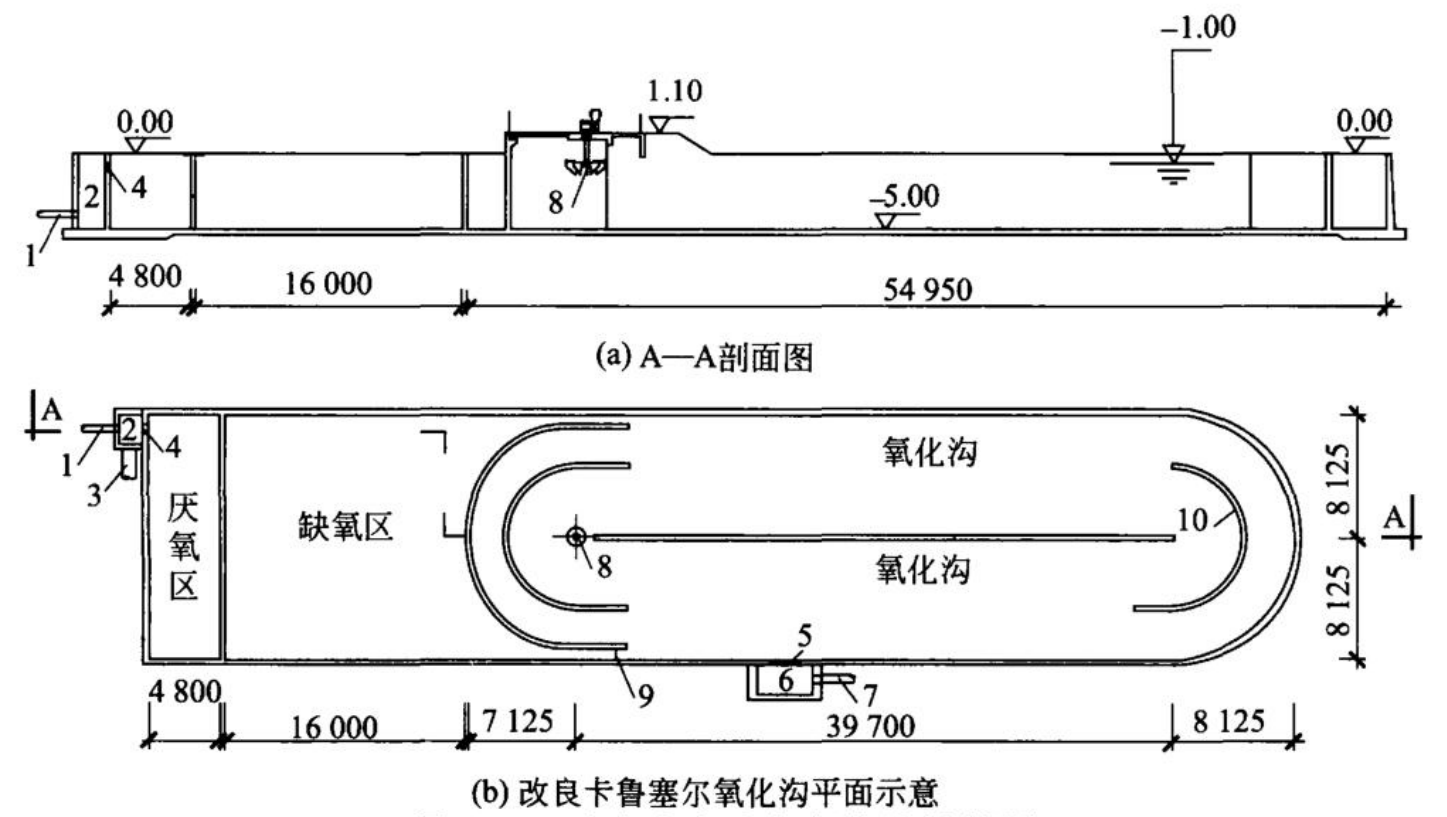
\includegraphics[width=\textwidth]{figures/Sketch of the modified Carrousel oxidation ditch.png}
  \caption{改良卡鲁塞尔氧化沟计算草图}
  \label{fig:carrousel-oxidation-ditch}
\end{figure}

\begin{enumerate}
	\item 好氧区容积 $V_1$
	\begin{align}
		V_1=\dfrac{Q(S_0-S_e)\theta_c Y_t}{1000X} &=\dfrac{35000\times(260-10)\times 20\times 0.7}{1000 \times 4} \;\text{m$^3$} \\
		&=\eval{\dfrac{35000\times(260-10)\times 20\times 0.7}{1000 \times 4}} \;\text{m$^3$} \notag
	\end{align}
	好氧区水力停留时间$t_1$为
	\begin{align}
		t_1=\dfrac{V_1}{Q}=\dfrac{30625}{35000} \;\text{d} =\eval{\dfrac{30625}{35000}} \;\text{d} =\eval{\dfrac{30625}{35000}*24} \;\text{h}
	\end{align}
	\item 缺氧区容积$V_2$缺氧区 容积采用反硝化动力学计算。
	\begin{align}
		V_2=\dfrac{0.001Q(N_k-N_{te})-0.12\Delta X_V}{K_{de}X}
		\label{eq:Volume of oxidation ditch hypoxic zone}
	\end{align}
	$V_2$——缺氧区有效容积,m$^3$;\par
	$N_k$——生物反应池进水总凯氏氮浓度,mg/L;\par
	$N_{te}$——生物反应池出水总氮浓度,mg/L;\par
	$\Delta X_V$——排出生物反应池系统的微生物量,kgMLVSS/d;\par
	$K_{de}$——脱氮速率,kgNO$_3^-$-N/(kgMLSS $\cdot$ d)。
	\begin{enumerate}
		\item 脱氮速率$K_{de(T)}$
		\begin{equation}
			K_{de(T)}=K_{de(20)}\theta^{T-20}
		\end{equation}
		$K_{de(20)}$——20℃时的脱氮速率,kgNO$_3^-$-N/(kgMLSS $\cdot$ d),取$K_{de(20)}$=0.06 kgNO$_3^-$-N/(kgMLSS $\cdot$ d);\par
		$\theta$——温度系数,取1.06;\par
		$T$——设计水温,℃,取8℃。

		所以,带入公式解得:
		\begin{align*}
			K_{de(T)}=K_{de(20)}\theta^{T-20}&=0.06\times 1.06^{8-20} \quad\text{kgNO$_3^-$-N/(kgMLSS $\cdot$ d)} \\ 
			&=0.030 \quad\text{kgNO$_3^-$-N/(kgMLSS $\cdot$ d)}
			% &=\eval{0.06\times 1.06^{8-20}}[3] \quad\text{kgNO$_3^-$-N/(kgMLSS $\cdot$ d)}
		\end{align*}

		\item 排出生物反应池系统的微生物量$\Delta X_V$
		\begin{equation}
			\Delta X_V=yY_t\dfrac{Q(S_0-S_e)}{1000}
		\end{equation}
		$Y_t$——污泥总产率系数,kgMLSS/kgBOD$_5$,取 0.7 kgMLSS/kgBOD$_5$;\par
		$y$——MLSS中MLVSS所占比例。取$y=0.6$;\par
		$S_0$——进水BOD$_5$浓度,mg/L;\par
		$S_e$——出水BOD$_5$浓度,mg/L。

		所以,带入公式解得:
		\begin{align*}
			\Delta X_V=yY_t\dfrac{Q(S_0-S_e)}{1000} &=0.6\times 0.7\times\dfrac{35000\times(260-10)}{1000} \quad\text{kgMLVSS/d} \\ 
			&=\eval{0.6\times 0.7\times\dfrac{35000\times(260-10)}{1000}} \quad\text{kgMLVSS/d} 
		\end{align*}

		\item 缺氧容积$V_2$
		
		将所求数据带入公式 \ref{eq:Volume of oxidation ditch hypoxic zone} 求解:
		\begin{align*}
			V_2=\dfrac{0.001Q(N_k-N_{te})-0.12\Delta X_V}{K_{de}X} &= \dfrac{0.001\times35000\times(45-15)-0.12\times 3675}{0.030\times 4.0} \;\text{m$^3$} \\
			&= \eval{\dfrac{0.001\times35000\times(45-15)-0.12\times 3675}{0.030\times 4.0}} \;\text{m$^3$} 
		\end{align*}
		则缺氧区水力停留时间$t_2$为
		\begin{align}
			t_2=\dfrac{V_2}{Q}=\dfrac{5075}{35000} \;\text{d} =\eval{\dfrac{5075}{35000}} \;\text{d} =\eval{\dfrac{5075}{35000}*24} \;\text{h} 
		\end{align}
	\end{enumerate}
	\item 厌氧区容积$V_3$,m$^3$
	
	取厌氧区水力停留时间$t_3=1.5$ h\footnote{《室外排水设计规范》(GB 50014-2006):厌氧区水力停留时间 $1\sim 2$ h。},则
	\begin{align*}
		V_3= Qt_3=\dfrac{35000}{24}\times 1.5 \;\text{m$^3$} =\eval{\dfrac{35000}{24}\times 1.5} \;\text{m$^3$} 
	\end{align*}

	\item 氧化沟总容积$V$及停留时间$t$
	\begin{equation}
		V=V_1+V_2+V_3 = 30625 + 5075 + 2187.5 \;\text{m$^3$} = \eval{30625 + 5075 + 2187.5} \;\text{m$^3$}
	\end{equation}
	\begin{equation}
		t=\dfrac{V}{Q}=\dfrac{37887.5}{35000} \;\text{d} = \eval{\dfrac{37887.5}{35000}} \;\text{d} = \eval{\dfrac{37887.5}{35000}*24} \;\text{h}
	\end{equation}

	\item 校核污泥负荷
	\begin{align}
		N=\dfrac{QS_0}{X_VV_1} &=\dfrac{35000\times \dfrac{260}{1000}}{2.4\times 30625} \quad\text{kgBOD$_5$/(kgMLVSS $\cdot$ d)} \\
		&=\eval{\dfrac{35000\times \dfrac{260}{1000}}{2.4\times 30625}} \quad\text{kgBOD$_5$/(kgMLVSS $\cdot$ d) (符合要求)} \notag
	\end{align}

	\item 剩余污泥量
	\begin{align} \label{eq:Amount of sludge remaining}
		\Delta X &=Y_tQ(S_0-S_e)-K_d V_1 X_V +fQ(SS_0-SS_e) \\
		&=0.7\times 35000 \times (260-10) \times 10^{-3} -0.05\times 30625 \times 4 \notag \\ 
		&\phantom{=} +0.6\times 35000\times (280-10) \times 10^{-3} \;\text{kg/d} \notag \\
		&= \eval{0.7\times 35000 \times (260-10) \times 10^{-3} -0.05\times 30625 \times 4+0.6\times 35000\times (280-10) \times 10^{-3}} \;\text{kg/d} \notag
	\end{align}
	则剩余1kgBOD$_5$产生污泥量
	\begin{align}
		\dfrac{\Delta X}{Q(S_0-S_e)} &= \dfrac{5670}{35000\times (260-10)\times 10^{-3}} \;\text{(kgDS/kgBOD$_5$)} \\
		&=\eval{\dfrac{5670}{35000\times(260-10)\times 10^{-3}}} \;\text{(kgDS/kgBOD$_5$)} \notag
	\end{align}

	\item 污⽔需氧量AOR

	因为 $a=1.47$,$b=4.57$,$c=1.42$,则
	\begin{align}
		\text{AOR} &=0.001 a Q(S_0-S_e)-c\Delta X_V +b[0.001Q(N_k-N_{ke})-0.12\Delta X_V] \\
		&\phantom{= } -0.62b\left[0.001Q(N_t-N_{ke}-N_{oe})-0.12\Delta X_V\right] \notag \\
		& = 0.001\times 1.47\times 35000\times(260-10)-1.42\times 3675  \notag \\
		& \phantom{= } +4.57\times\left[0.001\times 35000\times(45-5)- 0.12\times 3675\right] \notag \\
		&\phantom{= } -0.62\times4.57\times\left[0.001\times35000\times(45-5-10)-0.12\times 3675\right] \notag \\
		& = \eval{0.001\times 1.47\times 35000\times(260-10)-1.42\times 3675 +4.57\times\left[0.001\times 35000\times(45-5) - 0.12\times 3675\right]-0.62\times4.57\times\left[0.001\times35000\times(45-5-10)-0.12\times 3675\right]} \;\text{(kgO$_2$/d)} \notag
	\end{align}

最大需氧量与平均需氧量之比为1.58,则
\begin{align}
	\mathrm{AOR_{max}} &= 1.58 \text{AOR}=1.58 \times 10301.0894 \;\text{(kgO$_2$/d)} \\
	&= \eval{1.58 \times 10301.0894}[3] \;\text{(kgO$_2$/d)} \notag \\
	&= \eval{1.58 \times 10301.0894/24}[3] \;\text{(kgO$_2$/h)} \notag
\end{align}
\begin{align}
\text{去除1kgBOD$_5$需氧量} &= \dfrac{\mathrm{AOR_{max}}}{Q(S_0-S_e)} \\
&= \dfrac{16275.721}{35000 \times (260-10)\times 10^{-3}} \;\text{(kgO$_2$/kgBOD$_5$)} \notag \\
&=\eval{\dfrac{16275.721}{35000 \times (260-10)\times 10^{-3}}}[3] \;\text{(kgO$_2$/kgBOD$_5$)} \notag
\end{align}

	\item 氧化沟尺寸
	
	设氧化沟为2组,则单组氧化沟有效容积为
	\begin{equation}
		V_{\text{单}}=\dfrac{V}{2}=\dfrac{37887.5}{2} \;\text{m$^3$}=\eval{\dfrac{37887.5}{2}} \;\text{m$^3$}
	\end{equation}
	取氧化沟有效水深 $h=4$ m\footnote{《室外排水设计标准》(GB 50014-2021):氧化沟有效水深的确定应考虑曝气、混合、推流的设备性能,宜采用$3.5\sim 4.5$ m。},超高为 $h_0=1.0$ m\footnote{《室外排水设计标准》(GB 50014-2021):当好氧区的充氧器采用转刷、转碟时,氧化沟的设备平台高出设计水面宜为0.5 m;当采用竖轴表曝机时,宜为 $0.6 \;\text{m}\sim 0.8 \;\text{m}$,氧化沟的设备平台宜高出设计水面 $0.8 \;\text{m}\sim 1.2 \;\text{m}$。},则单组氧化沟面积为
	\begin{equation}
		A_{\text{单}}=\dfrac{V_{\text{单}}}{h}=\dfrac{18943.75}{4} \;\text{m$^2$}=\eval{\dfrac{18943.75}{4}}[2] \;\text{m$^2$}
	\end{equation}
	氧化沟高度为
	\begin{equation}
		H=h+h_0 = 4+1.0 \;\text{m} =5 \;\text{m}
	\end{equation}
	\begin{enumerate}
		\item 好氧区尺寸
		
		单组氧化沟好氧区容积
		\begin{equation}
			V_{1\text{单}}=\dfrac{V_1}{2}=\dfrac{30625}{2} \;\text{m$^3$} = \eval{\dfrac{30625}{2}} \;\text{m$^3$}
		\end{equation}
		好氧区面积
		\begin{equation}
			A_{1\text{单}}=\dfrac{V_{1\text{单}}}{h}=\dfrac{15312.5}{4} \;\text{m$^2$} = \eval{\dfrac{15312.5}{4}} \;\text{m$^2$}
		\end{equation}
		好氧区采用2沟道,单沟道宽度取 $b=8$ m,中间分隔墙厚度取 $d=0.25$ m。

		弯道部分面积(半圆)
		\begin{equation}
			A_{1\text{弯}}=2\cdot\dfrac{\pi b^2}{2} =2\times\dfrac{\pi\cdot 8^2}{2} \;\text{m$^2$} = \eval{2\times\dfrac{\pi\cdot 8^2}{2}}[2] \;\text{m$^2$}
		\end{equation}
		直线段部分面积
		\begin{equation}
			A_{1\text{直}}=A_{1\text{单}}-A_{1\text{弯}}=3828.125-200.96 \;\text{m$^2$} = \eval{3828.125-200.96} \;\text{m$^2$}
		\end{equation}
		直线部分长度
		\begin{equation}
			L_{1\text{直}} =\dfrac{A_{1\text{直}}}{2b} =\dfrac{3627.165}{2\times 8} \;\text{m} =\eval{\dfrac{3627.165}{2\times 8}}[3] \;\text{m}
		\end{equation}

		\item 缺氧区尺寸
		
		单组氧化沟缺氧区容积
		\begin{equation}
			V_{2\text{单}}=\dfrac{V_2}{2}=\dfrac{5075}{2} \;\text{m$^3$} = \eval{\dfrac{5075}{2}} \;\text{m$^3$}
		\end{equation}
		缺氧区面积
		\begin{equation}
			A_{2\text{单}}=\dfrac{V_{2\text{单}}}{h}=\dfrac{2537.5}{4} \;\text{m$^2$} = \eval{\dfrac{2537.5}{4}} \;\text{m$^2$}
		\end{equation}
		缺氧区宽度$B_2$与好氧区沟道同宽,则
		\begin{equation}
			B_2=b+d+b=8+0.25+8 \;\text{m} =16.25 \;\text{m}
		\end{equation}
		缺氧区长度
		\begin{equation}
			L_{2} =\dfrac{A_{2\text{单}}}{B_2} =\dfrac{634.375}{16.25} \;\text{m} =\eval{\dfrac{634.375}{16.25}}[3] \;\text{m}
		\end{equation}

		\item 厌氧区尺寸
		
		单组氧化沟厌氧区容积
		\begin{equation}
			V_{3\text{单}}=\dfrac{V_3}{2}=\dfrac{2187.5}{2} \;\text{m$^3$} = \eval{\dfrac{2187.5}{2}} \;\text{m$^3$}
		\end{equation}
		厌氧区面积
		\begin{equation}
			A_{3\text{单}}=\dfrac{V_{3\text{单}}}{h}=\dfrac{1093.75}{4} \;\text{m$^2$} = \eval{\dfrac{1093.75}{4}} \;\text{m$^2$}
		\end{equation}
		厌氧区长度$L_3$与好氧区沟道同宽
		\begin{equation}
			L_3=b+d+b=8+0.25+8 \;\text{m} =16.25 \;\text{m}
		\end{equation}
		厌氧区宽度
		\begin{equation}
			B_{3} =\dfrac{A_{3\text{单}}}{L_3} =\dfrac{273.4375}{16.25} \;\text{m} =\eval{\dfrac{273.4375}{16.25}}[3] \;\text{m}
		\end{equation}
	\end{enumerate}
\end{enumerate}


 % 氧化沟工艺部分
\subsection{二沉池}
\subsubsection{二沉池的选择}

普通辐流式二沉池的优点如下:
\begin{enumerate}
	\item 处理效率高:普通辐流式二沉池在处理污水时能够实现较高的沉降速度和较高的固液分离效率。通过合理的设计和操作,可以将污水中的悬浮颗粒和浮游生物有效地沉降到底部,从而实现高效的污水处理。
	\item 空间占用小:普通辐流式二沉池采用辐流式进出水方式,即进水和出水位于同一侧面,从而节省了空间。这对于一些空间受限的污水处理厂尤为重要,能够更好地满足设计要求。
	\item 操作维护简便:普通辐流式二沉池结构相对简单,没有复杂的机械设备或动力系统,因此操作和维护相对简单。这减少了运行成本和维护工作的复杂性,提高了处理厂的可靠性和稳定性。
	\item 适用性广泛:普通辐流式二沉池适用于各种规模的污水处理厂,无论是小型的社区处理厂还是大型的工业污水处理厂。它可以处理不同水质和污水特性的废水,具有较强的适应性和通用性。
	\item 抗负荷冲击能力强:普通辐流式二沉池在处理污水时具有较强的抗负荷冲击能力。它能够在短时间内应对污水负荷的变化,保持较高的处理效果,对于处理厂的稳定性和可靠性至关重要。
\end{enumerate}

综上所述,普通辐流式二沉池作为一种常用的污水处理工艺,具有高处理效率、小空间占用、简便的操作维护、广泛的适用性和强大的抗负荷冲击能力等优点。在设计污水处理厂时,选择普通辐流式二沉池是一个可靠和经济的选择,能够有效地处理污水并满足环境排放标准。


\subsubsection{计算数据与条件}

\begin{table}[H]
	\centering
	\caption{普通辐流式二沉池基础数据}
	\begin{tabular}{p{0.35\textwidth} *{3}{p{0.1\textwidth}}}
		\toprule
		参数    & 符号    & 值     & 单位 \\
		\midrule
		设计流量  & $Q$ & 35000 & m$^3$/d \\
		最大设计流量  & $Q_{max}$ & 58100 & m$^3$/d \\
		综合生活污水量变化系数 & $K_z$ & 1.66 &  \\
		\midrule
		氧化沟中悬浮固体浓度 & $X$    & 4000   & mg/L \\
		二沉池底流生物固体浓度 & $X_r$   & 10000   & mg/L \\
		污泥回流比 & $R$   & 100    & \% \\
		\bottomrule
	\end{tabular}%
	\label{tab:Basic data of ordinary radial secondary sedimentation tank}
\end{table}%

查阅刘振江和崔玉川主编的《城市污水厂处理设施设计计算》,得到普通辐流式沉淀池计算公式如下:

\begin{table}[H]
	\centering
	\caption{普通辐流式沉淀池计算公式\cite[p.224]{《城市污水厂处理设施设计计算(第三版)》}}
	\resizebox{\textwidth}{!}{%
	\begin{tabular}{l|l|l}
		\toprule
		名称    & 公式    & 符号说明  \\
		\midrule
		沉淀部分水面面积/m$^2$ & \makecell[l]{$F=\dfrac{Q_{max}}{nq}$\\$F\geqslant \dfrac{24(1+R)Q_0X}{G_L}$} & \makecell[l]{$Q_{max}$——最大设计流量,m$^3$/h \\
		$n$——池数,个 \\
		$q$——表面负荷,m$^3$/(m$^2\cdot$h) \\
		$R$——回流比 \\
		$Q_0$——单池设计流量,m$^3$/h \\
		$X$——混合液悬浮固体浓度,kg/m$^3$ \\
		$G_L$——极限固体通量,kg/(m$^2\cdot$d)} \\
		\midrule
		直径/m    & $D=\sqrt{\dfrac{4F}{\pi}}$    &   \\
		\midrule
		校核固体负荷/[kg/(m$^2\cdot$d)]   & $G = \dfrac{24(1+R)Q_0X}{F}$    &  \makecell[l]{G值一般可达150 kg/(m$^2\cdot$d)\\$Q_0$——单池设计流量,m$^3$/h} \\
		\midrule
		沉淀部分有效水深/m    & $h_2=qt$    & $t$——沉淀时间,h  \\
		\midrule
		污泥区的容积/m$^3$    & $V=\dfrac{2T(1+R)QX}{(X+X_r)\times 24}	$    & \makecell[l]{$Q$——平均日污水量,m$^3$/d \\
		$T$——贮泥时间,h \\
		$X_r$——沉淀池底流污泥浓度,kg/m$^3$}  \\
		\midrule
		污泥区高度/m    & \makecell[l]{$h_4=h_4'+h_4''+h_4'''$\\
		$h_4'=\dfrac{12}{\pi(D_1^2+D_1D_2+D_2^2)\times V_1}$\\
		$h_4''=\dfrac{12}{\pi(D^2+DD_1+D_1^2)\times V_2}$\\
		$h_4'''=\dfrac{V-V_1-V_2}{F}$}    & \makecell[l]{$V_1$——污泥斗容积,m$^3$ \\
		$V_2$——污泥斗以上圆锥体部分容积,m$^3$ \\
		$h_4'$——污泥斗的高度,m \\
		$h_4''$——圆锥体部分高度,m \\
		$h_4'''$——竖直段污泥部分的高度,m \\
		$D_1$——污泥斗上部的直径,m \\
		$D_2$——污泥斗下部的直径,m}  \\
		\midrule
		沉淀池总高/m   & $H=h_1+h_2+h_3+h_4$    & \makecell[l]{$h_1$——超高,m \\
		$h_3$——缓冲层高度,m}  \\
		\bottomrule
	\end{tabular}}
	\label{tab:Calculation formula of ordinary radiated sedimentation tank}%
\end{table}%


\subsubsection{主体设计计算}

\begin{figure}[H]
	\centering
	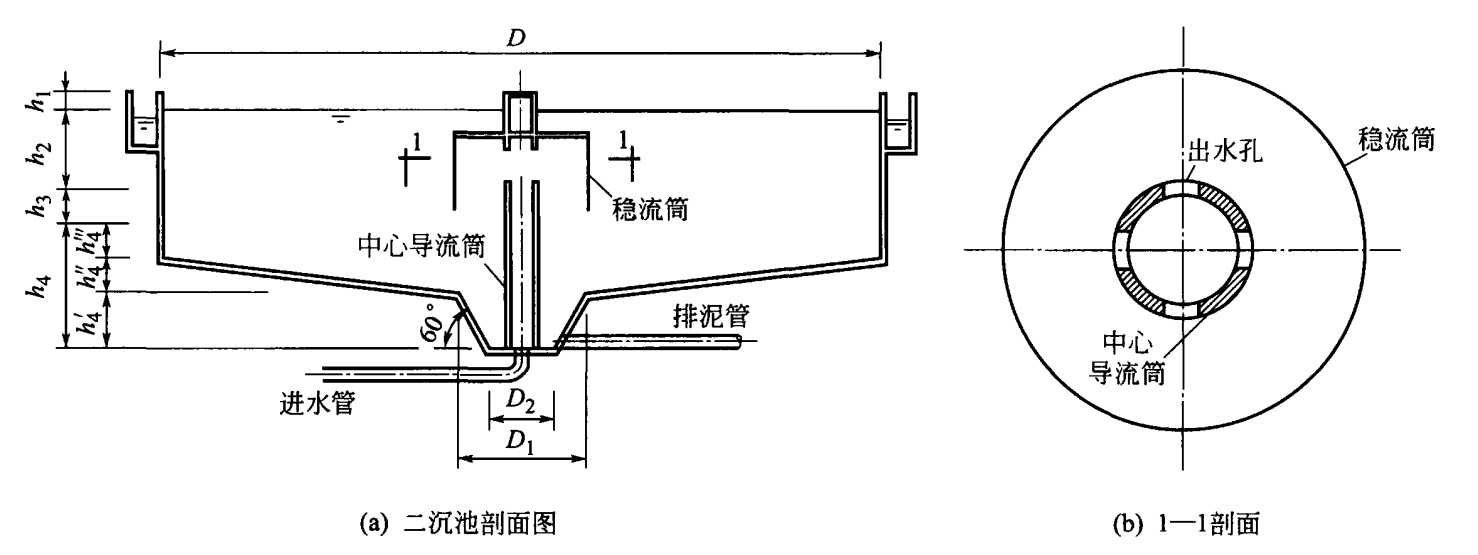
\includegraphics[width=\textwidth]{figures/Sketch of an ordinary radial type secondary sedimentation tank.png}
	\caption{普通辐流式二沉池计算草图\cite[p.225]{《城市污水厂处理设施设计计算(第三版)》}}
	\label{fig:Sketch of an ordinary radial type secondary sedimentation tank}
\end{figure}

\begin{enumerate}
	\item 沉淀部分水面面积 $F$
	
	根据生物处理段的特性,选取二沉池表面负荷 $q=0.7$ m$^3$/(m$^2\cdot$h)\footnote{普通辐流式沉淀池表面负荷一般不大于 2.5 m$^3$/(m$^2\cdot$h)。\cite{《城市污水厂处理设施设计计算(第三版)》}},设两座沉淀池即 $n=2$,则
	\begin{equation}
		F=\dfrac{Q_{max}}{nq} = \dfrac{58100}{2\times 0.7\times 24} \;\text{m$^2$} = \eval{\dfrac{58100}{2\times 0.7\times 24}}[2] \;\text{m$^2$}
	\end{equation}

	\item 池子直径 $D$
	
	\begin{align}
		D=\sqrt{\dfrac{4F}{\pi}} &= \sqrt{\dfrac{4\times 1729.17}{\pi}} \;\text{m} = \eval{\sqrt{\dfrac{4\times 1729.17}{\pi}}} \;\text{m} \\
		& \approx 47 \;\text{m(向上取整)} \notag
	\end{align}

	\item 校核固体负荷 $G$
	
	\begin{align}
		G = \dfrac{24(1+R)Q_0X}{F} & = \dfrac{24\times(1+100\%)\times 58100 \times 4}{1729.17 \times 2\times 24} \quad\text{kg/(m$^2\cdot$d)}  \\
		&= \eval{\dfrac{24\times(1+1)\times 58100 \times 4}{1729.17 \times 2\times 24}}[3] \quad\text{kg/(m$^2\cdot$d)} \notag \\
		% & \in [140,160] \quad\text{kg/(m$^2\cdot$d)(符合要求)}  \notag
		& \leqslant 150 \quad\text{kg/(m$^2\cdot$d)(符合要求)}  \notag
	\end{align}
	% \footnotetext{污泥固体负荷为 $140\sim 160$ kg/(m$^2\cdot$d)。\cite{《城市污水厂处理设施设计计算(第三版)》}}

	\item 沉淀部分的有效水深 $h_2$
	
	设沉淀时间 $t=3$ h,则
	\begin{equation}
		h_2=qt = 0.7 \times 3 \;\text{m} = 2.1 \;\text{m}
	\end{equation}

	\item 污泥区的容积 $V$
	
	设计采用周边传动的刮吸泥机排泥,污泥区容积按 2 h 贮泥时间确定,则
	\begin{align}
		V=\dfrac{2T(1+R)QX}{(X+X_r)\times 24} &= \dfrac{2\times 2\times (1+100\%)\times 35000\times 4000}{(4000+10000)\times 24} \;\text{m$^3$} \\
		& = \eval{\dfrac{2\times 2\times (1+1)\times 35000\times 4000}{(4000+10000)\times 24}}[2] \;\text{m$^3$} \notag
	\end{align}
	所以,每个沉淀池污泥区的容积 $V'=V/2=1666.67$ m$^3$。

	\item 污泥区高度 $h_4$
	\begin{enumerate}
		\item 污泥斗高度
		
		设池底的径向坡度为 $i = 0.05$,污泥斗底部直径 $D_2= 1.5$ m,上部直径 $D_1=3.0$ m,倾角 $\alpha=60^{\circ}$,则
		\begin{align}
			h_4' =\dfrac{D_1-D_2}{2}\cdot \tan{\alpha} = \dfrac{3.0-1.5}{2}\times \tan{60^{\circ}} \;\text{m} =\eval{\dfrac{3.0-1.5}{2}\times \tan{60/180*\pi}}[2] \;\text{m}
		\end{align}
		\begin{align}
			V_1 = \dfrac{\pi h_4'}{12}\cdot(D_1^2+D_1D_2+D_2^2) &= \dfrac{1.3 \pi}{12}\times(3.0^2+3.0\times 1.5+1.5^2) \;\text{m$^3$} \\
			&= \eval{\dfrac{\pi \times 1.3}{12}\times(3.0^2+3.0\times 1.5+1.5^2)}[2] \;\text{m$^3$} \notag
		\end{align}

		\item 圆锥体高度
		
		\begin{align}
			h_4'' =\dfrac{D-D_1}{2}\cdot i = \dfrac{47-3}{2}\times 0.05 \;\text{m} =\eval{\dfrac{47-3}{2}\times 0.05}[2] \;\text{m}
		\end{align}
		\begin{align}
			V_2 = \dfrac{\pi h_4''}{12}\cdot(D^2+DD_1+D_1^2) &= \dfrac{1.1 \pi}{12}\times(47^2+47\times 3.0+3.0^2) \;\text{m$^3$} \\
			&= \eval{\dfrac{\pi \times 1.1}{12}\times(47^2+47\times 3.0+3.0^2)}[2] \;\text{m$^3$} \notag
		\end{align}

		\item 竖直段污泥部分的高度
		
		\begin{align}
			h_4''' =\dfrac{V'-V_1-V_2}{F} = \dfrac{1666.67-5.36-679.34}{1729.17} \;\text{m} =\eval{\dfrac{1666.67-5.36-679.34}{1729.17}}[1] \;\text{m}
		\end{align}
		则污泥区的高度 $h$ 为
		\begin{align}
			h_4=h_4'+h_4''+h_4''' = 1.3+1.1+0.6 \;\text{m} =3.0 \;\text{m}
		\end{align}
	\end{enumerate}

	\item 沉淀池的总高度 $H$
	
	设超高 $h_1=0.3$ m,缓冲层高度 $h_3=0.5$ m,则
	\begin{align}
		H=h_1+h_2+h_3+h_4 = 0.3+2.1+0.5+3.0 \;\text{m} =\eval{0.3+2.1+0.5+3.0} \;\text{m}
	\end{align}
\end{enumerate}


\subsubsection{中心进水导流筒及稳流筒}
\begin{enumerate}
	\item 中心进水导流筒
	
	进水 $D_0=800$ mm,进水管流速 $v_0$ 为
	\begin{align}
		v_0 = \dfrac{4(1+R)Q_{max}}{n\pi D_0^2} = \dfrac{4\times(1+100\%)\times 58100}{2\pi \cdot 0.8^2 \times 86400} \;\text{m/s} =\eval{\dfrac{4\times(1+1)\times 58100}{2\pi \times 0.8^2 \times 86400}}[2] \;\text{m/s}
	\end{align}
	中心进水导流筒内流速取 $v_1=0.6$ m/s\footnote{中心进水导流筒内流速可达 1 m/s。},导流筒直径 $D_3$ 为
	\begin{align}
		D_3 = \sqrt{\dfrac{4(1+R)Q_{max}}{n\pi v_1}} &= \sqrt{\dfrac{4\times(1+100\%)\times 58100}{2\pi \cdot 0.6 \times 86400}}  \;\text{m} =\eval{\sqrt{\dfrac{4\times(1+1)\times 58100}{2\pi \cdot 0.6 \times 86400}}} \;\text{m} \\
		& \approx 1.20 \;\text{m(向上取整)}
	\end{align}
	中心进水导流筒设4个出水孔,出水孔尺寸 $B\times H=0.8 \;\text{m}\times 1.2 \;\text{m}$,出水孔流速 $v_2$ 为
	\begin{align}
		v_2 = \dfrac{(1+R)Q_{max}}{4nBH} &= \dfrac{(1+100\%)\times 58100}{4\times 2 \times 0.8 \times 1.2 \times 86400} \;\text{m/s} \\
		&=\eval{\dfrac{(1+1)\times 58100}{4\times 2 \times 0.8 \times 1.2 \times 86400}}[3] \;\text{m/s} \leqslant 0.2 \;\text{m/s} \notag
	\end{align}

	\item 稳流筒
	
	稳流筒用于稳定由中心筒流出的水流,防止对沉淀产生不利影响。稳流筒下缘淹没深度为水深的 $30\%\sim 70\%$,且低于中心导流筒出水孔下缘 0.3 m 以上。稳流筒内下降流速 $v_3$ 按最高时流量设计时一般控制在 $0.02\sim 0.03$ m/s之间,取 $v_3=0.03$,稳流筒内水流面积 $f$ 为
	\begin{equation}
		f=\dfrac{(1+R)Q_{max}}{nv_3} = \dfrac{(1+100\%)\times 58100}{2\times 0.03\times 86400} \;\text{m$^2$} = \eval{\dfrac{(1+1)\times 58100}{2\times 0.03\times 86400}}[2] \;\text{m$^2$}
	\end{equation}
	所以,稳流筒直径 $D_4$ 为
	\begin{align}
		D_4 = \sqrt{\dfrac{4f}{\pi}+D_3^2} &= \sqrt{\dfrac{4\times 22.42}{\pi}+1.2^2} \;\text{m} = \eval{\sqrt{\dfrac{4\times 22.42}{\pi}+1.2^2}} \;\text{m} \\
		& \approx 5.5 \;\text{m(向上保留一位小数)} \notag
	\end{align}

	\item 验算二沉池表面负荷
	
	二沉池有效沉淀区面积 $A$ 为
	\begin{align}
		A = \dfrac{\pi (D^2-D_4^2)}{4} = \dfrac{\pi (47^2-5.5^2)}{4} \;\text{m$^2$} = \eval{\dfrac{\pi (47^2-5.5^2)}{4}}[2] \;\text{m$^2$}
	\end{align}
	则二沉池实际表面负荷 $q'$ 为
	\begin{align}
		q' = \dfrac{Q_{max}}{nA} = \dfrac{58100}{2 \times 1711.19\times 24} \;\text{m$^3$/(m$^2\cdot$h)} = \eval{\dfrac{58100}{2 \times 1711.19\times 24}}[3]  \;\text{m$^3$/(m$^2\cdot$h)}
	\end{align}

	\item 验算二沉池固体负荷
	
	\begin{align}
		G' = \dfrac{(1+R)XQ_{max}}{1000nA} &= \dfrac{(1+100\%)\times 4000 \times 58100}{1000\times 2 \times 1711.19} \;\text{kg/(m$^2\cdot$d)} \\
		&= \eval{\dfrac{(1+1)\times 4000 \times 58100}{1000\times 2 \times 1711.19}}[2] \;\text{kg/(m$^2\cdot$d)} \notag
	\end{align}
\end{enumerate}



 % 二沉池部分
\subsection{污泥浓缩脱水}
加压溶气气浮法是一种广泛适用于处理不同水量、高浓度悬浮性污染物、油类、微生物、纸浆和纤维的先进处理方法。它已经在城镇污水处理厂中得到广泛应用,并且该工艺在工程实践中已经积累了丰富的经验。

该方法具有多项优势,包括高负荷率、卓越的处理效果和强大的处理能力,能够实现全自动连续运行。此外,通过灵活采用全溶气或部分回流溶气的方式,它还能够适应不同悬浮物浓度的废水处理需求。同时,该技术还能够有效地降低泥渣含水率,保证出水水质的优良。\cite{HJ2007-2010}

因此,在本次污泥浓缩设计中,我们选择了加压溶气气浮法作为处理方法,同时严格遵循中华人民共和国环境保护部《污水气浮处理工程技术规范》(HJ 2007-2010)的要求,以确保设计方案的科学性和可靠性。

\begin{figure}[H]
	\centering
	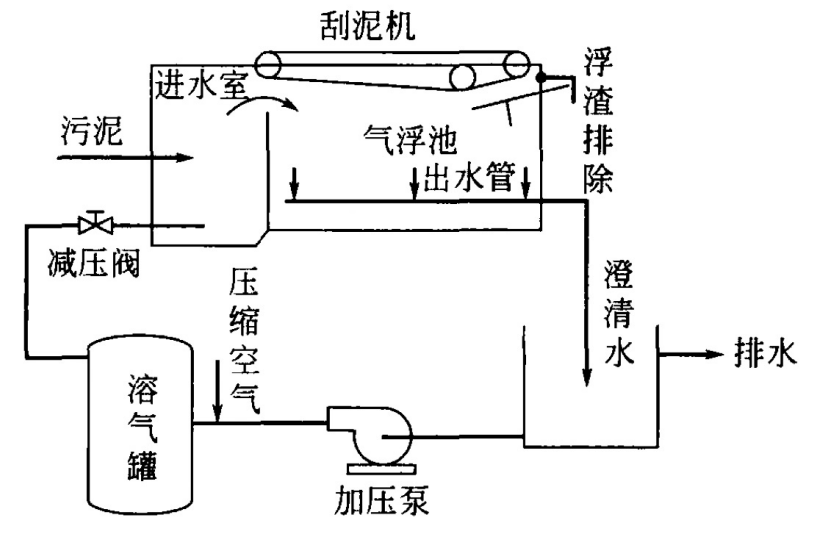
\includegraphics[width=0.8\textwidth]{figures/Sludge thickening process diagram.png}
	\caption{污泥浓缩流程简图}
	\label{fig:Sludge thickening process diagram}
\end{figure}


\subsubsection{基础数据}
% 回流溶气水的回流比(或溶气水比)应计算确定,一般为 $15\%\sim30\%$。\cite{HJ2007-2010}
% 查阅《室外排水设计标准》(GB 50014-2021),由生物反应池后二次沉淀池进入污泥浓缩池的污泥含水率为 $99.2\%\sim 99.6\%$ 时,浓缩后污泥含水率可为 $97.0\%\sim98.0\%$。
% 则数据汇总如下:
\begin{enumerate}
	\item 加压溶气气浮处理工艺中水温控制在20℃;
	\item 剩余污泥量 $\Delta X=5670$ kg/d (计算见公式 \ref{eq:Amount of sludge remaining} );
	\item 污水中悬浮物质量浓度,$S_a=2.6$ kg/m$^3$;
	\item 溶气罐设计工作压力一般为 $0.4\sim0.5$ MPa\cite{HJ2007-2010},则溶气压力取 $P=0.4 \;\text{MPa}=3.95 \;\text{atm}$;
	% \item 设进⼊污泥浓缩池的污泥含⽔率为 $99.6\%$;
	\item 回流溶气水的回流比或溶气水比(一般为 $15\%\sim30\%$\cite{HJ2007-2010}),$R =30 \%$。
	% \item 气固比 $\alpha$ 与悬浮颗粒的疏水性有关,一般情况下 $\alpha=0.005\sim 0.006$,通常由试验确定。% 在这里取 $\alpha=0.005$。
\end{enumerate}
因为气浮池的数量为2,则单个气浮池的剩余污泥流量 $Q$ 为
\begin{align}
	Q=\dfrac{\Delta X}{S_a}=\dfrac{5670}{2.6 \times 24 \times 2} \;\text{m$^3$/h} = \eval{\dfrac{5670}{2.6 \times 24 \times 2}}[3] \;\text{m$^3$/h}
\end{align}


\subsubsection{加压溶气气浮工艺指标计算}
\begin{enumerate}
	\item 气浮某种物质的气固比 $\alpha$
	
	\begin{equation}
		\alpha = \dfrac{\gamma C_s(fP-1)R}{S_a}
	\end{equation}
	$\alpha$——气浮某种物质的气固比;\par
	$\gamma$——空气容重,gL,见表 \ref{tab:The solubility of air in water};\par
	$C_s$——在一定温度下,一个大气压时的空气溶解度,mL/L $\cdot$ atm,见表 \ref{tab:The solubility of air in water};\par
	$f$——加压溶气系统的溶气效率,$f=0.8\sim0.9$;\par
	$P$——溶气压力,绝对压力,atm;\par
	$R$——试验条件下回流比或溶气水回流比,\%;\par
	$S_a$——污水中悬浮物质量浓度,kg/m$^3$;\par

	\begin{table}[H]
		\centering
		\caption{空气在水中的溶解度}
		\begin{tabular}{ccc}
		\toprule
		温度/℃  & 空气容重$\gamma$/(g/L) & 空气溶解度$C_s$(mL/L $\cdot$ atm) \\
		\midrule
		0     & 1.252 & 29.2 \\
		10    & 1.206 & 22.8 \\
		20    & 1.164 & 18.7 \\
		30    & 1.127 & 15.7 \\
		40    & 1.092 & 14.2 \\
		\bottomrule
		\end{tabular}%
		\label{tab:The solubility of air in water}%
	\end{table}%

	因为空气温度一般在20℃左右,所以空气容重取 $\gamma=1.164$ g/L,空气溶解度取 $C_s=18.7$ mL/L $\cdot$ atm,加压溶气系统的溶气效率取 $f=0.8$,则气浮某种物质的气固比 $\alpha$ 为
	\begin{align*}
		\alpha = \dfrac{\gamma C_s(fP-1)R}{S_a} &= \dfrac{1.164 \times 18.7\times (0.8 \times 3.95-1)\times 30\%}{2.6 \times 1000} \\
		&= \eval{\dfrac{1.164 \times 18.7\times (0.8 \times 3.95-1)\times 0.30}{2.6 \times 1000}}[4] \quad\text{(在 $0.005\sim 0.006$ 之间,满足条件)}
	\end{align*}

	\item 气浮池所需空气量 $Q_g$
	
	\begin{equation}\label{eq:alpga to Qg}
		\alpha = \dfrac{Q_g}{Q S_a}
	\end{equation}
	$Q_g$——气浮池所需空气量,kg/h;\par
	$Q$——气浮池处理水量,m$^3$/h; \par
	由上式 \ref{eq:alpga to Qg} 气固比 $\alpha$ 计算公式得,可以反向求出气浮池所需空气量 $Q_g$ 为
	\begin{align*}
		Q_g = \alpha Q S_a &= 0.0054 \times 45.433 \times 2.6 \;\text{kg/h} \\
		&= \eval{0.0054 \times 45.433 \times 2.6}[4] \;\text{kg/h}
	\end{align*}

	\item 所需空压机额定气量 $Q_g'$
	
	\begin{equation}
		Q_g'=\dfrac{\varPsi' Q_g}{60\gamma}
	\end{equation}
	$Q_g'$——所需空压机额定气量,m$^3$/min;\par
	$\varPsi'$——安全系数,$1.2\sim 1.5$。

	取安全系数 $\varPsi'=1.5$,则带入求得
	\begin{align*}
		Q_g'=\dfrac{\varPsi' Q_g}{60\gamma} &=\dfrac{1.5\times 0.6379}{60\times 1.164} \;\text{m$^3$/min} = \eval{\dfrac{1.5\times 0.6379}{60\times 1.164}}[4] \;\text{m$^3$/min}
	\end{align*}

	\item 溶气水量 $Q_r$
	
	\begin{equation} \label{eq:Reflux ratio R}
		R=\dfrac{Q_r}{Q}=\dfrac{1000\alpha S_a}{\gamma C_s(fP-1)}
	\end{equation}
	$Q_r$——溶气水量,m$^3$/h;\par

	由回流比 $R$ 计算公式 \ref{eq:Reflux ratio R} 得:
	\begin{equation}
		Q_r=QR = 45.433\times 30\% \;\text{m$^3$/h} = \eval{45.433\times 30/100}[3] \;\text{m$^3$/h}
	\end{equation}
\end{enumerate}


% \subsubsection{加压溶气气浮工艺指标计算 old}
% \begin{enumerate}
% 	\item 气浮池所需空气量 $Q_g$
	
% 	\begin{equation}
% 		Q_g=\dfrac{\gamma C_s(fP-1)RQ}{1000}
% 	\end{equation}
% 	$Q_g$——气浮池所需空气量,kg/h;\par
% 	$\gamma$——空气容重,gL,见表 \ref{tab:The solubility of air in water};\par
% 	$Q$——气浮池处理水量,m$^3$/h; \par
% 	$R$——试验条件下回流比或溶气水回流比,\%;\par
% 	$C_s$——在一定温度下,一个大气压时的空气溶解度,mL/L $\cdot$ atm,见表 \ref{tab:The solubility of air in water};\par
% 	$P$——溶气压力,绝对压力,atm;\par
% 	$f$——加压溶气系统的溶气效率,$f=0.8\sim0.9$。\par

	

% 	因为空气温度一般在20℃左右,所以空气容重取 $\gamma=1.164$ gL,空气溶解度取 $C_s=18.7$ mL/L $\cdot$ atm,加压溶气系统的溶气效率取 $f=0.8$,又因为回流比 $R$
% 	\begin{equation} \label{eq:Reflux ratio R}
% 		R=\dfrac{Q_r}{Q}=\dfrac{1000\alpha S_a}{\gamma C_s(fP-1)}
% 	\end{equation}
% 	$Q_r$——溶气水量,m$^3$/h;\par
% 	$S_a$——污水中悬浮物质量浓度,kg/m$^3$;\par
% 	$\alpha$——气浮某种物质的气固比。

% 	则
% 	\begin{align*}
% 		R =\dfrac{Q_r}{Q} =\dfrac{1000\alpha S_a}{\gamma C_s(fP-1)} &= \dfrac{1000\times 0.005\times 2.8}{1.164\times 18.7\times(0.8\times 3.95-1)} \\
% 		&= \eval{\dfrac{1000\times 0.005\times 2.8}{1.164\times 18.7\times(0.8\times 3.95-1)}}  \\
% 		& \approx 30 \;\text{\%(向上取整)}
% 	\end{align*}
% 	% 效验结果:根据《污水气浮处理工程技术规范》(HJ 2007-2010),回流溶气水的回流比(或溶气水比)应计算确定,一般为 $15\%\sim30\%$。符合要求。

% 	所以气浮池所需空气量 $Q_g$ 为
% 	\begin{align*}
% 		Q_g=\dfrac{\gamma C_s(fP-1)RQ}{1000} &=\dfrac{1.164\times 18.7\times(0.8\times 3.95-1)\times 30\%\times 117.42}{1000} \;\text{kg/h} \\
% 		&= \eval{\dfrac{1.164\times 18.7\times(0.8\times 3.95-1)\times 30/100 \times 117.42}{1000}}[3] \;\text{kg/h}
% 	\end{align*}

% 	% \item 气浮某种物质的气固比 $\alpha$ 
	
% 	% 气固比 $\alpha$ 与悬浮颗粒的疏水性有关,$\alpha=0.005\sim 0.006$,通常由试验确定。当无资料时,可按下式计算:
% 	% \begin{align}
% 	% 	\alpha &=\dfrac{Q_g}{QS_a}=\dfrac{\gamma C_s(fP-1)R}{1000S_a}
% 	% 	% & =\dfrac{1.656}{117.42\times 0.005} \;\text{kg/m$^3$} \notag \\
% 	% 	% & =\eval{\dfrac{1.656}{117.42\times 0.005}}[4] \;\text{kg/m$^3$} \notag 
% 	% \end{align}
% 	% $S_a$——污水中悬浮物质量浓度,kg/m$^3$。

% 	\item 所需空压机额定气量 $Q_g'$
	
% 	\begin{equation}
% 		Q_g'=\dfrac{\varPsi' Q_g}{60\gamma}
% 	\end{equation}
% 	$Q_g'$——所需空压机额定气量,m$^3$/min;\par
% 	$\varPsi'$——安全系数,$1.2\sim 1.5$。

% 	取安全系数 $\varPsi'=1.5$,则带入求得
% 	\begin{align*}
% 		Q_g'=\dfrac{\varPsi' Q_g}{60\gamma} =\dfrac{1.5\times 1.656}{60\times 1.164} \;\text{m$^3$/min} = \eval{\dfrac{1.5\times 1.656}{60\times 1.164}}[4] \;\text{m$^3$/min}
% 	\end{align*}

% 	\item 溶气水量 $Q_r$

% 	\begin{equation}
% 		Q_r=\dfrac{Q_g}{736fPK_T}
% 	\end{equation}
% 	$f$——溶气效率,对装阶梯环填料的溶气罐可取0.9;\par
% 	$P$——选定的溶气压力,atm;\par
% 	$K_T$——溶解度系数,可根据水温查表 \ref{tab:KT values at different temperatures} 而得。

% 	\begin{table}[H]
% 		\centering
% 		\caption{不同温度下的$K_T$值}
% 		\begin{tabular}{ccccccc}
% 		\toprule
% 		温度/℃  & 0     & 10    & 20    & 30    & 40    & 50 \\
% 		\midrule
% 		$K_T$值    & 0.038 & 0.029 & 0.024 & 0.021 & 0.018 & 0.016 \\
% 		\bottomrule
% 		\end{tabular}%
% 		\label{tab:KT values at different temperatures}%
% 	\end{table}%

% 	因为温度为20℃,所以溶解度系数 $K_T=0.024$,则溶气水量 $Q_r$ 为
% 	\begin{align*}
% 		Q_r=\dfrac{Q_g}{736fPK_T}=\dfrac{1.656}{736\times 0.8\times 3.95\times 0.024} \;\text{m$^3$/h} =\eval{\dfrac{1.656}{736\times 0.8\times 3.95\times 0.024}}[4] \;\text{m$^3$/h}
% 	\end{align*}

% 	由回流比 $R$ 计算公式 \ref{eq:Reflux ratio R} 得:
% 	\begin{equation}
% 		Q_r=QR = 117.42\times 30\% \;\text{m$^3$/h} = \eval{117.42\times 30/100} \;\text{m$^3$/h}
% 	\end{equation}
% \end{enumerate}


\subsubsection{气浮池接触室}
\begin{enumerate}
	\item 接触室表面积 $A_c$
	
	\begin{equation}
		A_c=\dfrac{Q+Q_r}{3600v_c}
	\end{equation}
	$A_c$——接触室表面积,m$^3$;\par
	$v_c$——水流平均速度,通常取 $10\sim20$ mm/s.

	取水流平均速度 $v_c=10 \;\text{mm/s} =0.01 \;\text{m/s}$,则接触室表面积 $A_c$ 为
	\begin{align*}
		A_c=\dfrac{Q+Q_r}{3600v_c}=\dfrac{45.433+13.63}{3600\times0.01} \;\text{m$^2$} = \eval{\dfrac{45.433+13.63}{3600\times0.01}}[4] \;\text{m$^2$}
	\end{align*}

	\item 接触室长度 $L$
	
	\begin{equation}
		L=\dfrac{A_c}{B_c}
	\end{equation}
	$L$——接触室长度,m;\par
	$B_c$——接触室宽度,m。

	因为平流式长宽比一般为 $2:1\sim3:1$\cite{HJ2007-2010},所以令 $L=2B_c$,则
	\begin{align*}
		L=\sqrt{2A_c} &=\sqrt{2\times 1.6406} \;\text{m} = \eval{\sqrt{2\times 1.6406}} \;\text{m} \\
		& \approx 1.82 \;\text{m(向上保留2位小数)}
	\end{align*}
	所以 $B_c=L/2=0.91$ m。

	\item 接触室堰上水深 $H_2$
	
	\begin{equation}
		H_2=B_c=0.91 \;\text{m}
	\end{equation}

	\item 接触室气水接触时间 $t_c$
	
	\begin{equation}
		t_c=\dfrac{H_1-H_2}{v_c}
	\end{equation}
	$t_c$——接触室气水接触时间,要求 $t_c>60$ s;\par
	$H_1$——气浮池分离室水深,通常为 $1.8\sim2.2$ m。

	取气浮池分离室水深 $H_1=1.8$ m,则
	\begin{align*}
		t_c=\dfrac{H_1-H_2}{v_c}=\dfrac{1.8-0.91}{0.01} \;\text{s} = \eval{\dfrac{1.8-0.91}{0.01}} \;\text{s($> 60$ s,满足要求)}
	\end{align*}
\end{enumerate}


\subsubsection{气浮分离室}
\begin{enumerate}
	\item 分离室表面积 $A_s$
	
	\begin{equation}
		A_s=\dfrac{Q+Q_r}{3600v_s}
	\end{equation}
	$A_s$——分离室表面积,m$^2$;\par
	$v_s$——分离室水流向下平均速度,通常为 $1\sim1.5$ mm/s。

	取分离室水流向下平均速度 $v_s=1.5$ mm/s,则分离室表面积 $A_s$ 为
	\begin{align*}
		A_s=\dfrac{Q+Q_r}{3600v_s} = \dfrac{45.433 + 13.63}{3600\times 1.5\times 10^{-3}} \;\text{m$^2$} = \eval{\dfrac{45.433 + 13.63}{3600\times 1.5\times 10^{-3}}}[3] \;\text{m$^2$}
	\end{align*}

	\item 分离室长度 $L_s$
	
	\begin{equation}
		L_s=\dfrac{A_s}{B_s}
	\end{equation}
	$L_s$——分离室长度,m;\par
	$B_s$——分离室宽度,m。

	因为对矩形池,分离室的长宽比一般取 $2:1\sim3:1$,所以令$L_s=2B_s$,则
	\begin{align*}
		L_s=\sqrt{2A_s} &=\sqrt{2\times 10.938} \;\text{m} = \eval{\sqrt{2\times 10.938}} \;\text{m} \\
		& \approx 4.68 \;\text{m(向上保留2位小数)}
	\end{align*}
	所以 $B_c=L/2=2.34$ m。

	\item 气浮池水深 $H$
	
	\begin{equation}
		H=v_s t
	\end{equation}
	$H$——气浮池水深,m;\par
	$t$——气浮池分离室停留时间,一般取 $10\sim 20$ min。

	取气浮池分离室停留时间 $t=20$ min,则气浮池水深 $H$ 为
	\begin{align*}
		H=v_s t=1.5 \times 10^{-3} \times 20 \times 60 \;\text{m} = \eval{1.5 \times 10^{-3} \times 20 \times 60} \;\text{m}
	\end{align*}

	\item 气浮池容积 $W$
	
	\begin{align}
		W= (A_c+A_s)\cdot H = (1.6406+10.938)\times 1.8 \;\text{m$^3$} = \eval{(1.6406+10.938)\times 1.8}[3] \;\text{m$^3$}
	\end{align}

	\item 总停留时间 $T$ 校核
	
	\begin{align}
		T=\dfrac{60\times W}{Q+Q_r} &= \dfrac{60\times 22.641}{45.433 + 13.63} \;\text{min} = \eval{\dfrac{60\times 22.641}{45.433 + 13.63}} \;\text{min} \\
		&\approx 23 \;\text{min} \notag
	\end{align}
\end{enumerate}


% \subsubsection{水位控制室}
% 水位控制室宽度 $B$ 不小于 900 mm,以便安装水位调节器,并利于检修。水位控制室可设于分离室一端,其长度等于分离室宽度。水位控制室深度一般与气浮分离室同深。


\subsubsection{溶气设备}
溶气罐应设安全阀,顶部最高点应装排气阀。溶气水泵进入溶气罐的入口管道应设除污过滤器。溶气罐底部应装快速排污阀。

溶气罐应设水位、压力仪表及自控装置。
\begin{enumerate}
	\item 压力溶气罐直径 $D_d$
	
	\begin{equation}
		D_d=\sqrt{\dfrac{4\times Q_r}{\pi I}}
	\end{equation}
	$D_d$——压力溶气罐直径,m;\par
	$I$——单位罐截面积的水力负荷,m;一般为 $80\sim 150$ m$^3$/(m$^2 \cdot$h),填料罐选用 $100\sim200$ m$^3$/(m$^2 \cdot$h)。

	取单位罐截面积的水力负荷 $I=80$ m$^3$/(m$^2 \cdot$h),如果只用1个溶气罐给2个池子充气,则压力溶气罐直径 $D_d$ 为
	\begin{align*}
		D_d=\sqrt{\dfrac{4\times Q_r}{\pi I}} &= \sqrt{\dfrac{4\times 13.63 \times 2}{\pi \times 80}} \;\text{m} = \eval{\sqrt{\dfrac{4\times 13.63\times 2}{\pi \times 80}}} \;\text{m} \\
		& \approx 750 \;\text{mm(向上取整)}
	\end{align*}

	\item 溶气罐高度 $Z$
	
	根据《污水气浮处理工程技术规范》(HJ 2007-2010),溶气罐一般为立式,设计高径比应大于 $2.5\sim 4$,有条件时取高值。则设计溶气罐高径比 $Z/D_d=4$,那么溶气罐高度 $Z$ 为
	\begin{equation}
		Z = 4 D_d = 4\times 0.750 \;\text{m} = 3.0 \;\text{m}
	\end{equation}
	又因为溶气罐高度 $Z$ 还可以通过下列公式计算:
	\begin{equation}
		Z = 2Z_1 + Z_2 + Z_3 + Z_4
	\end{equation}
	$Z$——溶气罐高度,m;\par
	$Z_1$——罐顶、底封头高度,m(根据罐直径而定);\par
	$Z_2$——布水区高度,一般取 $0.2\sim 0.3$ m;\par
	$Z_3$——贮水区高度,一般取 1.0 m;\par
	$Z_4$——填料层高度,当采用阶梯环时,可取 $1.0\sim 1.3$ m。

	溶气罐必要时可装填料,一般采用阶梯环填料,填料层高度应为罐高的 1/2,并不少于 0.8 m,液位控制高为罐高的 $1/4\sim 1/2$(从罐底计)\cite{HJ2007-2010}。所以取 $Z_2=0.3$ m,$Z_3=1.0$ m,$Z_4=Z/2 = 1.5$ m,则可以反求出罐顶、底封头高度 $Z_1$ 为
	\begin{align*}
		Z_1 = \dfrac{Z -(Z_2 + Z_3 + Z_4)}{2} &= \dfrac{3.0 -(0.3 + 1.0 + 1.5)}{2} \;\text{m} \\
		&= \eval{\dfrac{3.0 -(0.3 + 1.0 + 1.5)}{2}} \;\text{m}
	\end{align*}
	% 所以 $Z_4 = \dfrac{1}{2}Z = 1.4$ m $>0.8$ m(符合要求)。

	\item 溶气罐体积 $V_d$ 复核
	
	溶气罐水力停留时间 $t_d$ 应大于 $2 \sim 3$ min(有填料时取低值),并应计算确定;
	溶气水在溶气罐内停留时间:当无填料时 $t_d = 3\sim 3.5$ min;当有填料时 $t_d =2$ min。

	$\bullet $ 实际溶气罐体积
	\begin{align}
		V_d = \dfrac{\pi D_d^2}{4} \cdot Z = \dfrac{\pi \times 0.750^2}{4} \times 3.0 \;\text{m$^3$} = \eval{\dfrac{\pi \times 0.750^2}{4} \times 3.0}[3] \;\text{m$^3$}
	\end{align}
	$\bullet $ 理论溶气罐体积(用1个溶气罐给2个池子充气,取 $t_d =2$ min)
	\begin{align}
		V_d = Q_r \cdot t_d = \dfrac{13.63 \times 2 \times 2}{60} \;\text{m$^3$} = \eval{\dfrac{13.63 \times 2 \times 2}{60}}[3] \;\text{m$^3$}
	\end{align}

	% \item 溶气罐高径比 $Z/D_d$ 复核
	
	% 根据《污水气浮处理工程技术规范》(HJ 2007-2010),溶气罐一般为立式,设计高径比应大于 $2.5\sim 4$,有条件时取高值。
	
	% \begin{equation}
	% 	\dfrac{Z}{D_d} = \dfrac{3.0}{0.750} = \eval{\dfrac{3.0}{0.750}} \quad\text{(符合标准)}
	% \end{equation}
\end{enumerate}


% \subsubsection{气浮池集水管、集渣槽}
% \begin{enumerate}
% 	\item 气浮池集水管
	
% 	采用穿孔管,按分配流量及流速0.4~0.5 m/s确定管径。并令孔眼水头损失h=0.3 m,计算出孔口流速vo、孔眼尺寸和个数。
	
% 	\begin{equation}
% 		v_0 = \mu \sqrt{2gh}
% 	\end{equation}
% 	$v_0$——孔眼流速,m/s;\par
% 	$\mu$——孔眼流速系数。

% 	\item 集渣槽
	
% 	集渣槽断面设计可按单位时间的排泥量(包括抬高水位所带出的水量)进行选择。一般不小于200 mm,当浮渣浓度较高时,集渣槽需有足够的坡度倾向排泥口,一般应大于 $0.03\sim 0.05$。当集渣槽长度超过5 m时,应由两端向中间排泥。必要时可辅以冲洗水管。
% \end{enumerate}


% \subsubsection{溶气释放器}
% 溶气释放器可选择TJ型或TV型。溶气释放器个数 $n$ 计算公式如下:

% \begin{equation}
% 	n=\dfrac{Q_r}{q}
% \end{equation}
% $q$——选定溶气压力下单个释放器的出流量,m$^3$/h。

% 溶气水由溶气罐至释放器的管道上应设快开阀。

% 释放器应考虑快速拆卸装置。


% \subsubsection{刮渣机}
% 对于矩形气浮池应采用桥式刮渣机刮渣,跨度宜在 10 m以下,集渣槽的位置可在池的一端或两端;圆形气浮池宜采用行星式刮渣机,其适用范围在直径 $2\sim 10$ m,集渣槽位置可在圆池径向的任何部位。


\subsubsection{污泥脱水}
\paragraph{$\bullet $ 基础条件}~{}\par
污泥脱水设备:污泥真空转鼓过滤脱水机
\begin{enumerate}
    \item 该污水处理厂初沉污泥和剩余活性污泥消化后污泥产量 5636.2 m$^3$/d ;
    \item 污泥含水率 $p_0=99.6\%$ ;
    \item 经絮凝剂调质后,污泥比阻 $y=3\times 10^{11}$ m/kg ;
    \item 选用真空转鼓过滤机,要求脱水泥饼含水率达 80\% ;
    \item 过滤压力 $p=4.5\times 10^4$ N/m ;
    \item 过滤周期 $T=120$ s,泥饼形成时间 $t=36$ s ;
    \item 滤液动力黏度 $\mu =0.001$ N·s/m$^2$ 。
\end{enumerate}


\paragraph{$\bullet $ 设计计算}~{}\par
\begin{enumerate}
    \item 计算过滤产率 $L$ [kg/(m$^2$·s)]
    
    \begin{equation}\label{eq:Calculate filtration yield}
        L = \sqrt{\dfrac{2p \omega m}{\mu \gamma T}}
    \end{equation}
    式中:$m$——过滤机的浸液比,$m=t/T$;
    \newline\phantom{式中:}$\omega$——滤过单位体积的滤液在过滤介质上截留的干固体质量,g/mL,$\omega = \dfrac{C_g C_0}{100(C_g - C_0)}$;
    \newline\phantom{式中:}$C_0$——污泥干固体含量,\%;
    \newline\phantom{式中:}$C_g$——泥饼干固体含量,\%。

    因为 $t=36$ s,则过滤机的浸液比 $m$ 为
    \begin{equation}
        m=t/T = 36/120 = 0.3
    \end{equation}
    因为污泥干固体含量 $C_0=0.4\%$,污饼干固体含量 $C_g=20\%$,则滤过单位体积的滤液在过滤介质上截留的干固体质量 $\omega$ 为
    \begin{align}
        \omega = \dfrac{C_g C_0}{100(C_g - C_0)} &= \dfrac{20 \times 0.4}{100\times (20-0.4)} \;\text{g/mL} = \eval{\dfrac{20 \times 0.4}{100\times (20-0.4)}} \;\text{g/mL} \\
        &= \eval{\dfrac{20 \times 0.4}{100\times (20-0.4)}\times 1000}[3] \;\text{kg/m$^3$} \notag
    \end{align}
    将上述计算数据代入公式 \ref{eq:Calculate filtration yield} 得,计算过滤产率 $L$ 为
    \begin{align*}
        L = \sqrt{\dfrac{2p \omega m}{\mu \gamma T}} &= \sqrt{\dfrac{2 \times 4.5\times 10^{4} \times 4.082 \times 0.3}{0.001 \times 3\times 10^{11} \times 120}} \quad\text{kg/(m$^2$·s)} \\
        &= \eval{\sqrt{\dfrac{2 \times 4.5\times 10^{4} \times 4.082 \times 0.3}{0.001 \times 3\times 10^{11} \times 120}}} \;\;\text{kg/(m$^2$·s)} \notag \\
        &= \eval{\sqrt{\dfrac{2 \times 4.5\times 10^{4} \times 4.082 \times 0.3}{0.001 \times 3\times 10^{11} \times 120}}\times 3600}[2] \;\;\text{kg/(m$^2$·h)} \notag
    \end{align*}

    \item 过滤面积 $A$ (m$^2$)
    
    所需真空过滤机过滤面积为
    \begin{equation}
        A = \dfrac{af(1-p_0)Q\cdot 10^{3}}{L}
    \end{equation}
    式中:$a$——安全系数,取 $a=1.15$;
    \newline\phantom{式中:}$f$——考虑投加混凝剂污泥干重增加系数,取 $f=1.15$;
    \newline\phantom{式中:}$Q$——污泥量,m$^3$/h;
    \newline\phantom{式中:}$p_0$——污泥含水率,\%。

    已知日产污泥量 5636.2 m$^3$/d,脱水机每天工作两班,每班 8 h,则
    \begin{equation}
        \text{每小时污泥量} = \dfrac{5636.2}{2\times 8} \;\text{m$^3$/h} = \eval{\dfrac{5636.2}{2\times 8}}[2] \;\text{m$^3$/h}
    \end{equation}
    所以,过滤面积 $A$ 为
    \begin{align*}
        A = \dfrac{af(1-p_0)Q\cdot 10^{3}}{L} &= \dfrac{1.15\times 1.15\times (1-99.6\%)\times 352.26\times 10^{3}}{6.30} \;\text{m$^2$} \\
        &= \eval{\dfrac{1.15\times 1.15\times (1-0.996)\times 352.26\times 10^{3}}{6.30}}[2] \;\text{m$^2$}
    \end{align*}

    选用 5 台 G80-3.5 型转鼓真空过滤机,其中 1 台备用。每台脱水机过滤面积 80 m$^2$,转鼓直径 3.5 m$^2$,配电功率 5 kW。

    \item 附属设备的选择
    \begin{enumerate}[label=(\arabic*)]
        \item 真空泵。\\
        抽气量按 1 m$^2$ 介质面积 $0.5\sim 1.0$ m$^3$/min 估算,真空度 $200\sim 500$ mmHg (l mmHg $=133.3$ Pa),电机功率按 1 m$^3$/min 配 1.2 kW,则
		\begin{itemize}
			\item 抽气量 $Q = 40 \times 0.6 \;\text{m$^3$/min} = 24 \;\text{m$^3$/min}$
			\item 真空度 500 mmHg = 66661 Pa
			\item $\text{配电功率}=24\times 1.2 \;\text{kW} =28.8 \;\text{kW}$
		\end{itemize}
        故选用 2 台真空泵。

        \item 空压机。\\
        压缩气量按每 1 m$^2$ 介质 0.1 m$^3$/min 估算,压力 $0.2\sim 0.3$ MPa,电机功率按 1 m$^3$/min 配 4 kW 计算,则
		\begin{itemize}
			\item 压缩空气量 $Q=40 \times 0.1 \;\text{m$^3$/min} =4 \;\text{m$^3$/min}$,压力取 0.3 MPa
			\item 配电功率 $=4\times 4 \;\text{kW} =16 \;\text{kW}$
		\end{itemize}
        故空压机设置 2 台。

        \item 反冲洗泵。\\
        冲洗水量按 1 m$^2$ 介质面积 $0.8\sim 1.3$ L/s 计算,水压 $294\sim 343$ kPa ($3\sim 3.5$ kgf/cm$^2$)。
		\begin{itemize}
			\item 冲洗流量 $Q=40 \times 1.0 \;\text{L/s} =40 \;\text{L/s}$
			\item 冲洗水压 $H=343$ kPa (3.5 kgf/cm$^2$)
		\end{itemize}
        故反冲洗泵设置 2 台。
    \end{enumerate}
\end{enumerate}

 % 污泥浓缩部分
\subsection{消毒池}
\subsubsection{消毒方式的选择}

臭氧由3个氧原子组成,极不稳定,分解时产生初生态氧[O],具有极强的氧化能力,是除氟以外最活泼的氧化剂,对具有极强抵抗力的微生物如病毒、芽孢等具有很强的杀伤力。[O]还有很强的渗入细胞壁的能力,从而破坏细菌有机链状结构导致细菌的死亡。臭氧消毒的一般工艺流程如图  所示。

\begin{figure}[H]
	\centering
	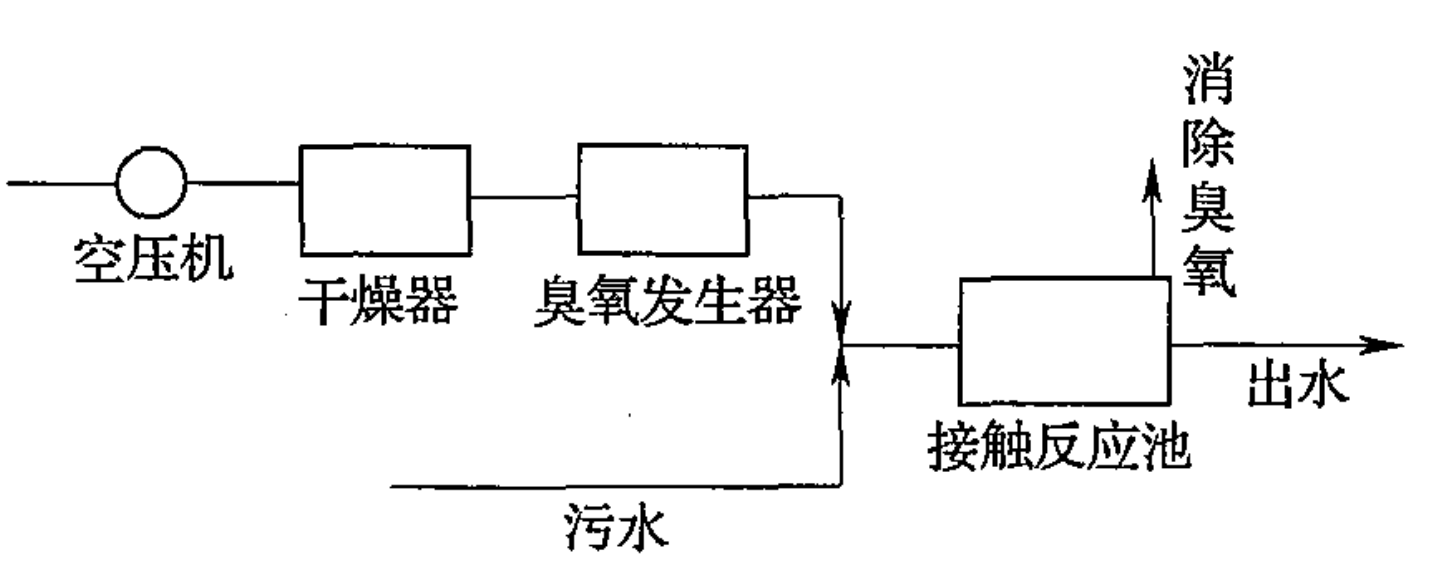
\includegraphics[width=0.6\textwidth]{figures/Ozone disinfection process.png}
	\caption{臭氧消毒流程\cite[p.387]{《第2册排水工程》}}
	\label{fig:Ozone disinfection process}
\end{figure}

臭氧在水中的溶解度仅为 10 mg/L左右,因此通人污水中的臭氧往往不可能全部被利用,为了提高臭氧的利用率,接触反应池最好建成水深为 $4\sim 6$ m的深水池,或建成封闭的几格串联的接触池,用管式或板式微孔扩散器扩散臭氧。臭氧消毒迅速,接触时间可采用15 min,能够维持的剩余臭氧量为 0.4 mg/L。接触池排出的剩余臭氧,具有腐蚀性,因此需作尾气破坏处理。臭氧不能贮存,需现场边发生边使用。臭氧消毒具有如下特点:
\begin{enumerate}
    \item 反应快,投量少,在水中不产生持久性残余,无二次污染;
    \item 适应能力强,在 $\text{pH} = 5.6 \sim 9.8$,水温 $0\sim 35$ ℃范围内,消毒性能稳定;
    \item 臭氧没有氯那样的持续消毒作用。
\end{enumerate}


\subsubsection{臭氧消毒接触池设计}

\begin{figure}[H]
	\centering
	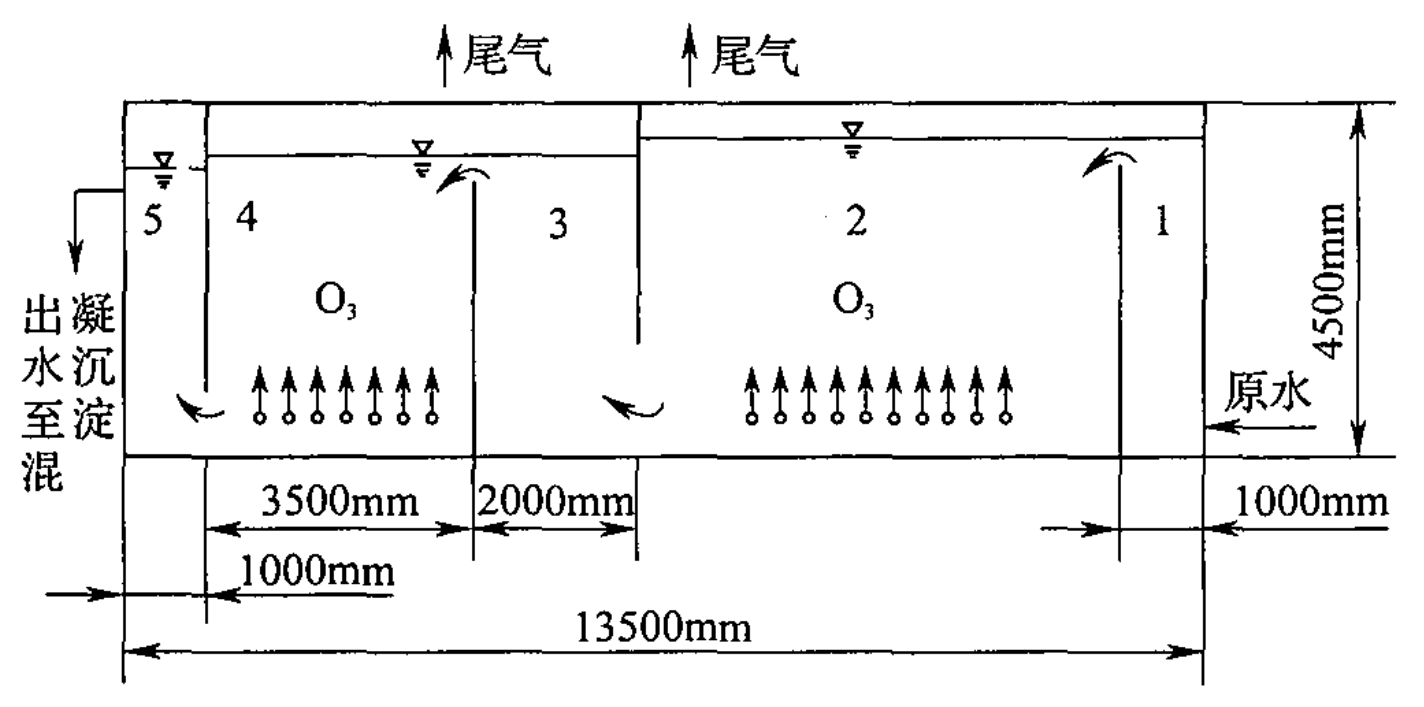
\includegraphics[width=0.8\textwidth]{figures/Ozone contact cell.png}
	\caption{臭氧接触池\cite[p.388]{《第2册排水工程》}}
	\label{fig:Ozone contact cell}
\end{figure}

\begin{enumerate}
	\item 容积
	
	\begin{equation}
		V=\dfrac{QT}{60}
	\end{equation}
	$V$——接触池容积,m$^3$;\par
	$Q$——所需消毒的污水流量,m$^3$/h;\par
	$T$——水力停留时间,mln,一般取 $5\sim 15$ min。

	因为 $Q_{max}=58100 \;\text{m$^3$/d}$ ,取水力停留时间 $T=9$ min ,则臭氧消毒接触池容积为
	\begin{align*}
		V = \dfrac{Q_{max}T}{60} = \dfrac{58100\times 9}{60\times 24} \;\text{m$^3$} = \eval{\dfrac{58100\times 9}{60\times 24}} \;\text{m$^3$} 
	\end{align*}

	\item 尺寸设计
	
	设池宽为 6 m ,其余尺寸如图 \ref{fig:Ozone contact cell} 所示,则其容积为
	\begin{align}
		V &= 6 \times 4.5 \times 13.5 \;\text{m$^3$} = \eval{6 \times 4.5 \times 13.5} \;\text{m$^3$} \\
		& > 363.125 \;\text{m$^3$(满足有效停留时间要求)} \notag
	\end{align}

	\item 1、3、5室的水流速度 $v_1$、$v_3$、$v_5$ 计算
	
	\begin{align}
		v_1 = v_5 = \dfrac{58100}{24}\times \dfrac{10^2}{3600\times 6\times 1.0} \;\text{cm/s} = \eval{\dfrac{58100}{24}\times \dfrac{10^2}{3600\times 6\times 1.0}}[3] \;\text{cm/s}
	\end{align}
	\begin{align}
		v_3 = \dfrac{1}{2}v_1 = \eval{\dfrac{11.208}{2}} \;\text{cm/s}
	\end{align}
\end{enumerate}


\subsubsection{臭氧发生器所需空气量}
\begin{enumerate}
	\item 臭氧需要量
	
	\begin{equation}
		D = 1.06\alpha Q 
	\end{equation}
	$D$——臭氧需要量,g/h;\par
	$\alpha$——臭氧投加量 g/m$^3$;\par
	$1.06$——安全系数;\par
	$Q$——所需消毒的污水流量,m$^3$/h。

	取最大投加臭氧量 $\alpha=2$ g/m$^3$,则臭氧需要量为
	\begin{align*}
		D = 1.06\alpha Q_{max} = 1.06\times 2 \times \dfrac{58100}{24} \;\text{g/h} = \eval{1.06\times 2 \times \dfrac{58100}{24}}[3] \;\text{g/h}
	\end{align*}

	\item 臭氧化所需空气量
	
	取臭氧化空气的臭氧含量 $c=10$ g/m$^3$,则臭氧化所需空气量为
	\begin{equation}
		V_{\text{干}} = \dfrac{D}{c} = \dfrac{5132.167}{10} \;\text{m$^3$/h} = \eval{\dfrac{5132.167}{10}} \;\text{m$^3$/h}
	\end{equation}
\end{enumerate}

 % 消毒池部分
\subsection{提升泵房}
提升泵泵房是污水处理厂中的一个重要设施,用于将污水从低处提升到高处,以便进行后续的处理和排放。


\subsubsection{水泵总扬程估算}
选泵前总扬程计算\cite[p.189]{《第2册排水工程》}:
\begin{equation}
	H=H_{ss}+H_{sd}+\sum{h_{s}}+\sum{h_{d}}
\end{equation}
式中:$H_{ss}$——吸水高度,为集水池内最低水位与水泵轴线之高差,m;
\newline\phantom{式中:}$H_{sd}$——压水高度,为泵轴线与输水最高点(即压水管出口处)之高差,m;
\newline\phantom{式中:}$\sum{h_{s}}$和$\sum{h_{d}}$——污水通过吸水管路和压水管路中的水头损失(包括沿程损失和局部损失),m。

根据《室外排水设计标准》的规定,污水泵设计扬程应根据设计流量时集水池水位与出水管渠水位差、水泵管路系统水头损失及安全水头三部分确定。
本项目设计参数如下表 \ref{tab:Lay out the design parameters} 所示:

\begin{table}[H]
	\centering
	\caption{布置设计参数}
	\begin{tabular}{cc}
	\toprule
	位置信息  & 标高(m) \\
	\midrule
	厂区设计地坪绝对标高 & 498.00 \\
	污水处理厂进水泵房处污水进水管管底标高 & 493.15 \\
	排水河流的最高水位 & 494.40 \\
	排水河流最低水位 & 491.80 \\
	常年平均水位 & 493.00 \\
	集水池池底标高 & 492.00 \\
	\bottomrule
	\end{tabular}%
	\label{tab:Lay out the design parameters}
\end{table}

\begin{enumerate}
	\item 集水池水位与出水管渠水位差 $H_{ss}+H_{sd} = \Delta H$
	
	% 出水管渠水位以及集水池水位的不同组合,可组成不同的扬程,设计流量时,出水管渠水位与集水池设计水位之差加上管路系统水头损失和安全水头为设计扬程;设计最小流量时,出水管渠水位与集水池设计最高水位之差加上管路系统水头损失和安全水头为最低工作扬程;	设计最大流量时,出水管渠水位与集水池设计最低水位之差 1 m 上管路系统水头损失和安全水头为最高工作扬程。安全水头一般为 $0.3 \sim 0.5$ m。
	
	设出水管管绝对标高 503.00 m,则
	\begin{align}
		H_{ss}+H_{sd} &= \Delta H \\
		&= 503.00-492.00-1.00 \;\text{m} \notag \\
		&= \eval{503-492-1} \;\text{m} \notag
	\end{align}

	\item 构筑物水头损失
	
	各构筑物水头损失见下表 \ref{tab:Loss of head of the structure} :
	\begin{table}[H]
		\centering
		\caption{构筑物水头损失}
		\begin{tabular}{cc}
		\toprule
		构筑物名称 & 水头损失(m) \\
		\midrule
		格栅    & 0.5 \\
		% 膜格栅   & 0.9 \\
		曝气沉砂池 & 0.5 \\
		氧化沟 & 0.6 \\
		二沉池   & 0.3 \\
		污泥浓缩池   & 0.9 \\
		消毒池   & 0.3 \\
		管路系统水头损失 & 1.0 \\
		\bottomrule
		\end{tabular}%
		\label{tab:Loss of head of the structure}
	\end{table}
	则可以求出各构筑物水头总损失 $\sum{h_{s}}+\sum{h_{d}} = \sum\limits_{i=1}^{n}\Delta P$:
	\begin{align}
		\sum{h_{s}}+\sum{h_{d}} &= \sum_{i=1}^{n}\Delta P \\
		&= 0.5+0.5+0.6+0.3+0.9+0.3+1.0 \;\text{m} \notag \\
		&= \eval{0.5+0.5+0.6+0.3+0.9+0.3+1.0} \;\text{m} \notag
	\end{align}

	\item 安全水头 $H_{\text{安全水头}}$
	
	由于污水泵站一般扬程较低,局部损失占总损失的比重较大,所以不可忽略。考虑到污水泵在使用过程中因效率下降和管道中阻力增加而增加的能量损失,在确定泵扬程时,可增大 $1 \sim 2$ m 安全扬程。则安全水头取 $H_{\text{安全水头}}=2$ m。
\end{enumerate}
故水泵总扬程估算为
\begin{align*}
	H &= H_{ss}+H_{sd}+\sum{h_{s}}+\sum{h_{d}} \\
	&= \Delta H + \sum\limits_{i=1}^{n}\Delta P + H_{\text{安全水头}} \\
	&= 10+4.1+2 \;\text{m} \\
	&= \eval{10+4.1+2} \;\text{m}
\end{align*}


\subsubsection{提升泵的选型}

因为设计最大流量 $Q_{max}=58100$ m$^3$/d,泵的个数为4\footnote{《室外排水设计标准》(GB 50014-2021):水泵台数不应少于2台,且不宜大于8台。},则每个泵的提升量为:
\begin{equation}
	Q_{\text{泵}}=\dfrac{Q_{max}}{4}=\dfrac{58100}{4}\;\text{m$^3$/d} =\eval{\dfrac{58100}{4}} \;\text{m$^3$/d}
\end{equation}

设水泵吸水管流速为 $v_0=1$ m/s \footnote{《室外排水设计标准》(GB 50014-2021):水泵吸水管设计流速宜为0.7 m/s $\sim$ 1.5 m/。},
出水管流速为 $v_1=2$ m/s \footnote{《室外排水设计标准》(GB 50014-2021):水泵出水管设计流速宜为0.8 m/s $\sim$ 2.5 m/s。}。
% \cite[p.39]{GB500142021}
根据《给水排水设计手册第 11 册常用设备(第三版)》,结合实际情况及计算所得的流量,选用 QXG 型潜水给水泵,其流量范围为 $50 \sim 3000$ m$^3$/h,扬程范围为 $5.5 \sim 65$ m,功率范围为 $7.5 \sim 250$ kW,可输送物理化学性质类似于水的液体,适用于城市、工厂、矿山、电站的给水排水和农田排涝灌溉等。QXG 型潜水给水泵类型如下表 \ref{tab:QXG type submersible feed pump} 所示:

\begin{table}[H]
	\centering
	\caption{QXG型潜水给水泵\cite{QXG型潜水给水泵}}
	\resizebox{\textwidth}{!}{
	\begin{tabular}{ccccccccccc}
	\toprule
	序号    & 规格型号  & 流量(Q)m$^3$/h & 扬程(H)m & 泵效率($\eta$)\% & 配套功率(P)kw & 转速(n)r/min & 口径(DN)$\phi$mm & 机座号   & 自耦装置型号 & 重量(W)kg \\
	\midrule
	1     & QXG300-5.5-7.5 & 300   & 5.5   & 70    & 7.5   & 980   & 150   & M160  & 150GAK & 280 \\
	2     & QXG50-32-11 & 50    & 32    & 75    & 11    & 1470  & 100   & M160  & 100GAK & 280 \\
	3     & QXG250-11-11 & 250   & 11    & 80.5  & 11    & 980   & 150   & M160  & 150GAK & 280 \\
	4     & QXG250-15-15 & 250   & 15    & 80.5  & 15    & 1470  & 150   & M160  & 150GAK & 280 \\
	5     & QXG400-9-15 & 400   & 9     & 80    & 15    & 1470  & 200   & M160  & 200GAK & 280 \\
	6     & QXG250-18-18.5 & 250   & 18    & 80    & 18.5  & 1470  & 150   & M180  & 150GAK & 450 \\
	7     & QXG400-11-18.5 & 400   & 11.5  & 80.5  & 18.5  & 1470  & 200   & M180  & 200GAK & 450 \\
	8     & QXG70-60-22 & 70    & 60    & 75    & 22    & 2900  & 100   & M180  & 100GAK & 500 \\
	9     & QXG140-35-22 & 140   & 35    & 80    & 22    & 1470  & 150   & M180  & 150GAK & 500 \\
	10    & QXG160-30-22 & 160   & 30    & 80    & 22    & 1470  & 150   & M180  & 150GAK & 500 \\
	11    & QXG250-21-22 & 250   & 21    & 79.5  & 22    & 1470  & 150   & M180  & 150GAK & 500 \\
	12    & QXG400-15-22 & 400   & 15    & 80    & 22    & 1470  & 200   & M180  & 200GAK & 500 \\
	13    & QXG600-9-22 & 600   & 9     & 82    & 22    & 980   & 250   & M200  & 250GAK & 600 \\
	14    & QXG250-27-30 & 250   & 27    & 76    & 30    & 980   & 200   & M225  & 200GAK & 800 \\
	15    & QXG400-18.5-30 & 400   & 18.5  & 80.5  & 30    & 980   & 200   & M225  & 200GAK & 800 \\
	16    & QXG600-12.5-30 & 600   & 12.5  & 82    & 30    & 980   & 250   & M225  & 250GAK & 800 \\
	17    & QXG900-8.5-30 & 900   & 8.5   & 83    & 30    & 980   & 250   & M225  & 250GAK & 800 \\
	18    & QXG250-33-37 & 250   & 33    & 75    & 37    & 1470  & 150   & M225  & 150GAK & 800 \\
	19    & QXG400-22-37 & 400   & 22    & 80    & 37    & 1470  & 200   & M225  & 200GAK & 800 \\
	20    & QXG600-15.5-37 & 600   & 15.5  & 80    & 37    & 1470  & 250   & M225  & 250GAK & 800 \\
	21    & QXG900-10-37 & 900   & 10    & 82    & 37    & 980   & 300   & M250  & 300GAK & 1200 \\
	22    & QXG1100-8-37 & 1100  & 8     & 82    & 37    & 980   & 300   & M250  & 300GAK & 1200 \\
	23    & QXG250-40-45 & 250   & 40    & 74    & 45    & 1470  & 200   & M225  & 200GAK & 1000 \\
	24    & QXG400-27-45 & 400   & 27    & 79    & 45    & 1470  & 200   & M225  & 200GAK & 800 \\
	25    & QXG600-18-45 & 600   & 18    & 80    & 45    & 1470  & 250   & M225  & 250GAK & 800 \\
	26    & QXG900-12.5-45 & 900   & 12.5  & 82    & 45    & 1470  & 300   & M225  & 300GAK & 800 \\
	27    & QXG1350-8.5-45 & 1350  & 8.5   & 83    & 45    & 740   & 400   & M280  & 400GAK & 1500 \\
	28    & QXG250-49-55 & 250   & 49    & 73    & 55    & 1470  & 200   & M250  & 200GAK & 1200 \\
	29    & QXG400-32.5-55 & 400   & 32.5  & 78    & 55    & 1470  & 200   & M250  & 200GAK & 1200 \\
	30    & QXG600-22-55 & 600   & 22    & 80    & 55    & 1470  & 250   & M250  & 250GAK & 1200 \\
	\bottomrule
	\end{tabular}}
	\label{tab:QXG type submersible feed pump}
\end{table}
\begin{table}[H]
	\centering
	\caption*{续表 \ref{tab:QXG type submersible feed pump} : QXG型潜水给水泵\cite{QXG型潜水给水泵}}
	\resizebox{\textwidth}{!}{
	\begin{tabular}{ccccccccccc}
	\toprule
	序号    & 规格型号  & 流量(Q)m$^3$/h & 扬程(H)m & 泵效率($\eta$)\% & 配套功率(P)kw & 转速(n)r/min & 口径(DN)$\phi$mm & 机座号   & 自耦装置型号 & 重量(W)kg \\
	\midrule
	31    & QXG900-15-55 & 900   & 15    & 82    & 55    & 1470  & 300   & M250  & 300GAK & 1500 \\
	32    & QXG1350-10-55 & 1350  & 10    & 83    & 55    & 980   & 400   & M280  & 400GAK & 1500 \\
	33    & QXG400-44-75 & 400   & 44    & 77.5  & 75    & 1470  & 200   & M280  & 200GAK & 1500 \\
	34    & QXG600-30-75 & 600   & 30    & 80    & 75    & 1470  & 250   & M280  & 250GAK & 1500 \\
	35    & QXG900-21-75 & 900   & 21    & 82    & 75    & 1470  & 300   & M280  & 300GAK & 1500 \\
	36    & QXG1350-14-75 & 1350  & 14    & 83    & 75    & 980   & 400   & M315  & 400GAK & 2300 \\
	37    & QXG2100-9-75 & 2100  & 9     & 84    & 75    & 590   & 500   & M315  & 500GAK & 2500 \\
	38    & QXG350-60-90 & 350   & 60    & 80    & 90    & 1470  & 200   & M280  & 200GAK & 1500 \\
	39    & QXG400-53-90 & 400   & 53    & 77    & 90    & 1470  & 200   & M280  & 200GAK & 1500 \\
	40    & QXG600-36-90 & 600   & 36    & 79    & 90    & 1470  & 250   & M280  & 250GAK & 1500 \\
	41    & QXG900-25-90 & 900   & 25    & 82    & 90    & 1470  & 300   & M280  & 300GAK & 1500 \\
	42    & QXG1350-17-90 & 1350  & 17    & 83    & 90    & 980   & 400   & M315  & 400GAK & 2300 \\
	43    & QXG2100-11-90 & 2100  & 11    & 84    & 90    & 740   & 500   & M315  & 500GAK & 2500 \\
	44    & QXG600-44-110 & 600   & 44    & 79    & 110   & 1470  & 250   & M315  & 250GAK & 2100 \\
	45    & QXG900-30-110 & 900   & 30    & 82    & 110   & 1470  & 250   & M315  & 250GAK & 2100 \\
	46    & QXG1350-20-110 & 1350  & 20    & 83    & 110   & 980   & 400   & M315  & 400GAK & 2300 \\
	47    & QXG2100-13-110 & 2100  & 13    & 84    & 110   & 980   & 400   & M315  & 400GAK & 2300 \\
	48    & QXG3000-9.5-110 & 3000  & 9.5   & 85    & 110   & 740   & 500   & M315  & 500GAK & 2500 \\
	49    & QXG400-65-132 & 400   & 65    & 75    & 132   & 1470  & 250   & M315  & 250GAK & 2100 \\
	50    & QXG600-52-132 & 600   & 52    & 78.5  & 132   & 1470  & 250   & M315  & 250GAK & 2100 \\
	51    & QXG900-35-132 & 900   & 35    & 81    & 132   & 1470  & 250   & M315  & 250GAK & 2100 \\
	52    & QXG1350-24-132 & 1350  & 24    & 83    & 132   & 980   & 400   & M315  & 400GAK & 2300 \\
	53    & QXG2100-16-132 & 2100  & 16    & 84    & 132   & 980   & 400   & M315  & 400GAK & 2300 \\
	54    & QXG3000-11-132 & 3000  & 11    & 85    & 132   & 740   & 500   & M315  & 500GAK & 2500 \\
	55    & QXG600-60-160 & 600   & 60    & 80.5  & 160   & 1470  & 250   & M315  & 250GAK & 2100 \\
	56    & QXG900-43-160 & 900   & 43    & 80.5  & 160   & 1470  & 300   & M315  & 300GAK & 2200 \\
	57    & QXG1350-30-160 & 1350  & 30    & 83    & 160   & 1470  & 400   & M315  & 400GAK & 2300 \\
	58    & QXG2100-19-160 & 2100  & 19    & 84    & 160   & 980   & 500   & M315  & 500GAK & 2500 \\
	59    & QXG3000-14-160 & 3000  & 14    & 85    & 160   & 740   & 500   & M355  & 500GAK & 3800 \\
	60    & QXG600-65-185 & 600   & 65    & 80    & 185   & 1470  & 250   & M355  & 250GAK & 3500 \\
	61    & QXG900-50-185 & 900   & 50    & 80    & 185   & 980   & 300   & M355  & 300GAK & 3750 \\
	62    & QXG1350-34-185 & 1350  & 34    & 82.5  & 185   & 980   & 400   & M355  & 400GAK & 3950 \\
	63    & QXG2100-22-185 & 2100  & 22    & 84    & 185   & 980   & 500   & M355  & 500GAK & 3950 \\
	64    & QXG3000-16-185 & 3000  & 16    & 85    & 185   & 980   & 500   & M355  & 500GAK & 3950 \\
	65    & QXG900-54-200 & 900   & 54    & 82    & 200   & 980   & 300   & M355  & 300GAK & 3950 \\
	66    & QXG1350-37-200 & 1350  & 37    & 82    & 200   & 980   & 400   & M355  & 400GAK & 3950 \\
	67    & QXG2100-24-200 & 2100  & 24    & 84    & 200   & 980   & 500   & M355  & 500GAK & 3950 \\
	68    & QXG3000-17-200 & 3000  & 17    & 85    & 200   & 980   & 500   & M355  & 500GAK & 3950 \\
	69    & QXG900-59-220 & 900   & 59    & 82    & 220   & 980   & 300   & M355  & 300GAK & 4100 \\
	70    & QXG1350-41-220 & 1350  & 41    & 82    & 220   & 980   & 400   & M355  & 400GAK & 4100 \\
	71    & QXG2100-27-220 & 2100  & 27    & 84    & 220   & 980   & 500   & M355  & 500GAK & 4100 \\
	72    & QXG3000-19-220 & 3000  & 19    & 85    & 220   & 980   & 500   & M355  & 500GAK & 4100 \\
	73    & QXG2100-30-250 & 2100  & 30    & 83.5  & 250   & 980   & 500   & M355  & 500GAK & 4250 \\
	74    & QXG3000-22-250 & 3000  & 22    & 85    & 250   & 980   & 500   & M355  & 500GAK & 4250 \\
	\bottomrule
	\end{tabular}}
\end{table}

根据设计需求(流量:$Q'_{\text{泵}}>Q_{\text{泵}}=14525/24 \;\text{m$^3$/h}\approx 606 \;\text{m$^3$/h}$;扬程:$H'>H=16.1 \;\text{m} \approx 17 \;\text{m}$),再结合上表 \ref{tab:QXG type submersible feed pump},选用 5 台 QXG900-21-75 型潜水给水泵,四用一备。

\begin{table}[H]
	\centering
	\caption{QXG900-21-75 型潜水给水泵性能参数}
	\resizebox{\textwidth}{!}{
	\begin{tabular}{ccccccccccc}
	\toprule
	序号    & 规格型号  & 流量(Q)m$^3$/h & 扬程(H)m & 泵效率($\eta$)\% & 配套功率(P)kw & 转速(n)r/min & 口径(DN)$\phi$mm & 机座号   & 自耦装置型号 & 重量(W)kg \\
	\midrule
	35    & QXG900-21-75 & 900 & 21 & 82    & 75    & 1470  & 300   & M280  & 300GAK & 1500 \\
	\bottomrule
	\end{tabular}}
	\label{tab:QXG900-21-75 submersible feed pump performance parameters}
\end{table}


\subsubsection{水泵最大安装高度}

泵的允许几何安装高度与多方面条件有关\cite{水泵最大安装高度如何计算},公式如下:
\begin{equation}
	\left[H_g\right]=\dfrac{p_e}{\rho g}-\dfrac{p_v}{\rho g}-\left[NPSH\right]-h_w
\end{equation}
式中:$\left[H_g\right]$——泵的允许几何安装高度,m;(计算结果供设计时利用,实际安装高度需低于允许安装高度)
\newline\phantom{式中:}$p_e$——吸水水面压力,Pa;(为吸水水面的大气压,海拔越高大气压越低)
\newline\phantom{式中:}$p_v$——饱和蒸汽压力,Pa;(与水温有关,水温越高,饱和蒸汽压力越高)
\newline\phantom{式中:}$\rho$——流体的密度,kg/m$^3$;
\newline\phantom{式中:}$g$——重力加速度,9.81 m/s$^2$;
\newline\phantom{式中:}$\left[NPSH\right]$——水泵的允许汽蚀余量,m;(与水泵性能有关,由水泵厂家提供)
\newline\phantom{式中:}$h_w$——吸入管路中的水头损失,m。

\begin{table}[H]
  \centering
  \caption{不同海拔时的大气及对应的水头高度\cite{水泵最大安装高度如何计算}}
    \begin{tabular}{ccc}
    \toprule
    海振高度(m) & 大气压力(kPa) & 水头高度(m) \\
    \midrule
    -600  & 110.85 & 11.3 \\
    0     & 101.32 & 10.3 \\
    200   & 99.08 & 10.1 \\
    500   & 95.16 & 9.7 \\
    100   & 90.25 & 9.2 \\
    1500  & 84.36 & 8.6 \\
    2000  & 79.46 & 8.1 \\
    3000  & 70.63 & 7.2 \\
    4000  & 61.8  & 6.3 \\
    5000  & 53.95 & 5.5 \\
    \bottomrule
    \end{tabular}
	\label{tab:The atmosphere at different altitudes and the corresponding head height}
\end{table}%

\begin{table}[H]
  \centering
  \caption{不同温度时水的饱和蒸汽压对应水头高度\cite{水泵最大安装高度如何计算}}
    \begin{tabular}{ccc}
    \toprule
    水温(℃) & 饱和蒸汽压力(kPa) & 水头高度(m) \\
    \midrule
    10    & 1.23  & 0.125 \\
    20    & 2.34  & 0.238 \\
    30    & 4.24  & 0.433 \\
    40    & 7.37  & 0.752 \\
    50    & 12.33 & 1.272 \\
    60    & 19.92 & 2.066 \\
    70    & 31.16 & 3.249 \\
    80    & 47.36 & 4.97 \\
    90    & 70.1  & 7.406 \\
    100   & 101.32 & 10.786 \\
    \bottomrule
    \end{tabular}
	\label{tab:The saturated vapor pressure of water at different temperatures corresponds to the height of the head}
\end{table}%

因为该城镇污水处理厂的海拔高度为:$490 \sim 520$ m,吸水水面压力为当地大气压,,由表 \ref{tab:The atmosphere at different altitudes and the corresponding head height} 查得海拔 500 m处大气压力
\[\dfrac{p_e}{\rho g} = 9.7 \;\text{m}\]
气温:最冷月平均为 5℃,最热月平均为 32.5℃,最冷月水温在 $8 \sim 12$ 摄氏度取。由表 \ref{tab:The saturated vapor pressure of water at different temperatures corresponds to the height of the head} 估算出水的饱和蒸汽压头为
$$\dfrac{p_v}{\rho g} = \dfrac{1.272-0.752}{40-30}\times (32.5-30)+0.752 \;\text{m} = \eval{(1.272-0.752)/(40-30)\times (32.5-30)+0.752} \;\text{m}$$
QXG900-21-75 水泵汽蚀余量为 $$\text{[NPSH]r}=3.29 \;\text{m}$$
欲在海拔 500 m高度的地方工作,该地区夏季最高水温为32.5℃,取吸水管的水头损失为 $$h_w = 1 \;\text{m}$$
则该泵在当地的运行几何安装高度 [Hg] 计算如下:
\begin{align*}
	\left[H_g\right] &=\dfrac{p_e}{\rho g}-\dfrac{p_v}{\rho g}-\left[NPSH\right]-h_w \\
	&= 9.7-0.882-3.29-1 \;\text{m} \\
	&= \eval{9.7-0.882-3.29-1} \;\text{m}
\end{align*}


\subsubsection{集水池的计算}
污水泵站集水池的容积与进入泵站的流量变化情况、泵的型号、台数及其工作制度、泵站操作性质、启动时间等有关。同时,集水池的容积在满足安装格栅和吸水管的要求、保证泵工作时的水力条件以及能够及时将流人的污水抽走的条件下,应尽量小些。因为缩小集水池的容积,不仅能降低泵站的造价,还可减轻集水池污水中大量杂物的沉积和腐化。此外,污泥泵房集水池的容积应按一次排入的污泥量和污泥泵抽送能力计算确定。活性污泥泵房集水池的容积,应按排入的回流污泥量、剩余污泥量和污泥泵抽送能力计算确定。最后,在集水池中设置冲洗装置和清泥设施\cite{GB500142021}。

取$t_{min}=6$ min\footnote{《室外排水设计标准》(GB 50014-2021):污水泵站集水池的容积不应小于最大一台水泵 5 min的出水量。},则集水池的容量为
\begin{align}
	W = Q_{\text{泵}}\cdot t_{min}=\dfrac{14525}{24\times 60} \times 6 \;\text{m$^3$} =\eval{\dfrac{14525}{24\times 60} \times 6}[3] \;\text{m$^3$}
\end{align}

因为栅后槽总高度 $H=1.016$ m,栅前水深 $h=0.63$ m,进水渠宽 $B_1=1.26$ m,又因为“设计最高水位 = 进水管充满高度 + 水位保留高度”,则设置进水管充满高度为 0.63 m ,水位保留高度(泵的安装高度 $[H_g]=4.528$ m)为 4 m,取集水坑坑深为 600 mm\footnote{《室外排水设计标准》(GB 50014-2021):集水池池底应设置集水坑,坑深宜为 500 mm $\sim$ 700 mm。}。所以,可计算设计最高水位为
\begin{align}
	\text{设计最高水位} &= \text{进水管充满高度} + \text{水位保留高度} \\
	&= 0.63 + 4 \;\text{m} \notag \\
	&= \eval{0.63+4} \;\text{m} \notag
\end{align}


% \subsubsection{泵房布置}
% 泵房布置水泵房布置宜符合以下要求:
% \begin{enumerate}
% 	\item 水泵房的平面布置水泵布置宜采用单行布置,主要机组的布置和通道宽度,应满足机电设备安装、运行和操作的要求,即水泵机组基础间的净距不宜小于1.0m ,机组突出部分与墙壁的净距不宜小于1.2m,主要通道宽度不宜小于1.5m;配电箱前面的通道宽度,低压配电时不宜小于1.5m,高压配电时不宜小于 2.0m;当采用在配电箱后检修时,配电箱后距墙的净距不宜小于1.0m;有电动起重机的泵房内,应有吊装设备的通道。
% 	\item 水泵房的高程布置泵房各层层高应根据水泵机组、电气设备、起吊装置、安装、运行和检修等因素确定。水泵机组基座应按水泵的要求设置,并应高出地坪 0.lm 以上;泵房内地面敷设管道时,应根据需要设置跨越设施,若架空敷设时,不得跨越电气设备和阻碍通道,通行处的管底距地面不宜小于 2.0m;当泵房为多层时,楼板应设置吊物孔,其位置应在起吊设备的工作范围内,吊物孔尺寸应按所需吊装的最大部件外形尺寸每边放 0.2m 以上。
% \end{enumerate}

% 泵站室外地坪标高应按城镇防洪标准确定,并符合规划部门要求。泵房室内地坪应比室外地坪高 $0.2 \sim 0.3$ m 。易受洪水淹没地区的泵站,其人口处设计地面标高应比设计洪水位高 0.5m 以上,当不能满足上述要求时,可在人口处设置闸槽墩临时性防洪措施。
 % 泵站(房)设计部分
% \subsection{除臭装置}
\newpage
\section{厂区总图设计}
\subsection{厂区管道}
\subsubsection{厂区管道分类}
厂区主要管道有污水管,污泥管,空气管,厂区给水管,厂区排水管,厂区自用水
管,雨水管等。
\begin{enumerate}
	\item 污水管:\\
	污水管是污水处理厂中最主要的管线,它将各处理单元连接起来,起到承上启下的作用。
	\item 污泥管:\\
	污泥管输送污泥,也是主要管线,其输送成分主要由氧化沟产生的剩余污泥和后续系统分离出的污泥组成,该管线设计考虑污泥含水率低,尽量提高污泥流速,避免淤积,尽量少转弯,力求平直。
	\item 空气管:\\
	空气管道主要为需要曝气的单元输送空气,连接至鼓风机房并分别通入曝气沉砂池和卡鲁塞尔氧化沟好氧区。
	\item 工厂排水管:\\
	厂区还设有排水管将厂区废水回流至处理前端,使其进入系统。在厂区自用水管厂内设置厂区自用水管,管线布置主要考虑各生产构筑物冲洗水、绿化用水、生产加药稀释水等。为了防止污染,应设于污水污泥管之上,故设置浅层。
	\item 雨水管:\\
	厂内雨水经地面径流收集进入厂区雨水管,再经雨水泵提升排出厂外。主要沿厂区道路铺设管线。
\end{enumerate}


\subsubsection{进水管渠的计算}
\begin{figure}[H]
	\centering
	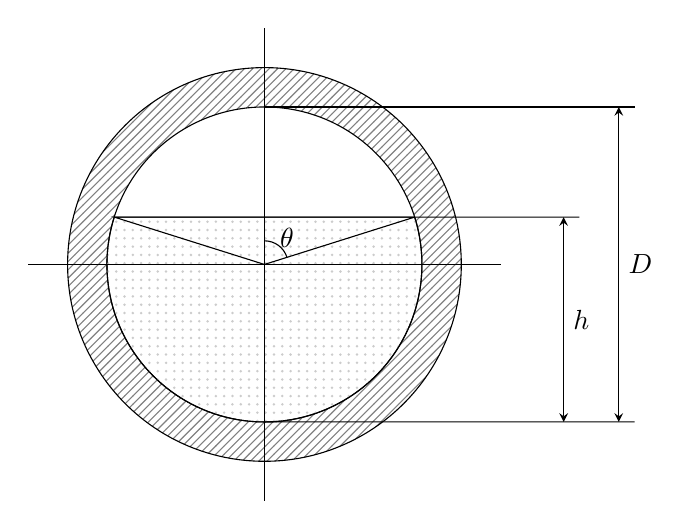
\begin{tikzpicture}
		\draw[pattern=north east lines, pattern color=black!50] (0,0) circle (2.5cm); % 绘制圆
		\draw[black, fill=white] (0,0) circle (2cm); % 绘制圆
		
		\foreach \mytheta in {17.5} {
			\draw[pattern=dots, pattern color=black!20] (\mytheta:2cm) -- (180-\mytheta:2cm) arc (-\mytheta-180:\mytheta:2cm);

			\foreach \r in {3} {
				\draw (-\r,0) -- (\r,0);
				\draw (0,-\r) -- (0,\r);
			}
			\draw (\mytheta:0.3cm) arc (\mytheta:90:0.3cm); % 绘制扇形
			\node[above] at (\mytheta:0.3cm) {$\theta $};
		
			\draw (\mytheta:2cm) -- (0,0) -- (180-\mytheta:2cm) -- (4,{sin(\mytheta)*2});
			\draw (-90:2cm) -- (4.7,-2);
			\draw[stealth-stealth] (3.8,{sin(\mytheta)*2}) -- (3.8,-2);
			\node[right] at (3.8,{sin(\mytheta)-1}) {$h$};
		
			\draw (0,2) -- (4.7,2);
			\draw[stealth-stealth] (4.5,2) -- (4.5,-2);
			\node[right] at (4.5,0) {$D$};
		}
	\end{tikzpicture}
	\caption{进水管径计算草图}
	\label{fig:Inlet pipe diameter calculation sketch}
\end{figure}

进水管渠的流量应按下式计算\cite[p.20]{GB500142021}:
$$Q=Av$$
由上图 \ref{fig:Inlet pipe diameter calculation sketch} 所示,因为充满度 $\lambda =\dfrac{h}{D}$,设半径为 $r$,则 $D=2r$,$h=2\lambda r$,得
\begin{align*}
	S_{\text{三角形}} &=(2\lambda -1)r\sqrt{r^2 - (2\lambda -1)^2r^2} \\
	\theta &= \arccos{\dfrac{(2\lambda -1)r}{r}} = \arccos{(2\lambda -1)} \\
	S_{\text{扇形}} &=\dfrac{2\pi-2\theta}{2\pi}\pi r^2 = \left[\pi-\arccos{(2\lambda -1)}\right]r^2
\end{align*}
所以,总水流有效断面面积为
\begin{align}
	A &= S_{\text{三角形}} + S_{\text{扇形}} \notag \\
	&=\left[(2\lambda -1)\sqrt{1 - (2\lambda -1)^2} +\pi-\arccos{(2\lambda -1)}\right]  r^2
\end{align}
为满足后续格栅处理工艺要求,取定流速为 $v=0.85$ m/s\footnote{《室外排水设计标准》(GB 50014-2021):污水过栅流速宜采用 0.6 m/s $\sim$ 1.0 m/s。},假设充满度 $\lambda =0.65$,并将公式$Q=Av$和流量 $Q_{max}=58100$ m$^3$/d,带入可求得管道半径为
\begin{align}
	r &= \sqrt{\dfrac{1}{(2\lambda -1)\sqrt{1 - (2\lambda -1)^2} +\pi-\arccos{(2\lambda -1)}}\cdot\dfrac{Q_{max}}{v}} \\
	&= \sqrt{\dfrac{1}{(2\times 0.65 -1)\sqrt{1 - (2\times 0.65 -1)^2} +\pi-\arccos{(2\times 0.65 -1)}}\times\dfrac{58100}{86400}\times\dfrac{1}{0.85}} \;\text{m} \notag \\
	&= \eval{\sqrt{\dfrac{1}{(2\times 0.65 -1)\sqrt{1 - (2\times 0.65 -1)^2} +\pi-\arccos{(2\times 0.65 -1)}}\times\dfrac{58100}{86400}\times\dfrac{1}{0.85}}}[5] \;\text{m} \notag
\end{align}
所以,求得管径为
\begin{align*}
	D=2r &=2\times 0.60496 \;\text{m}=\eval{2\times 0.60496 * 1000} \;\text{mm} \\
	&\approx  1200\;\text{mm(管径取整)}
\end{align*}


当管径取$D=1200$ mm时,可以反算出进水管道内的实际充满度:
% \begin{align} % 实际流速
% 	v=\dfrac{Q}{A}&=\dfrac{Q_{max}}{\left[(2\lambda -1)\sqrt{1 - (2\lambda -1)^2} +\pi-\arccos{(2\lambda -1)}\right]\dfrac{D^2}{4}} \\
% 	&=\dfrac{58100}{86400}\times\dfrac{1}{\left[(2\times 0.65 -1)\sqrt{1 - (2\times 0.65 -1)^2} +\pi-\arccos{(2\times 0.65 -1)}\right]\times\dfrac{1.2^2}{4}} \;\text{m/s} \notag \\
% 	&=\eval{\dfrac{\dfrac{58100}{86400}}{\left[(2\times 0.65 -1)\sqrt{1 - (2\times 0.65 -1)^2} +\pi-\arccos{(2\times 0.65 -1)}\right]\times\dfrac{1.2^2}{4}}}[3] \;\text{m/s} \notag
% \end{align}
\begin{align}
	A=\left[(2\lambda -1)\sqrt{1 - (2\lambda -1)^2} +\pi-\arccos{(2\lambda -1)}\right]  r^2 = \dfrac{Q_{max}}{v}
\end{align}
考虑到等式较为复杂,求解实际充满度 $\lambda$ 会比较麻烦,而且最大流量$Q_{max}$和$v$都是确定的值,那么总水流有效断面面积$A$为定值。
% 再根据上式可知,充满度$\lambda$会管道半径$r$成反比。因为实际管径比理论管径要小($D_{\text{实际}}<D_{\text{理论}}$),所以实际充满度会比理论充满度大($\lambda_{\text{实际}}>\lambda_{\text{理论}}$),则
因为实际充满度的范围一定会在0与1之间($\lambda\in [0,1]$),则利用Python使用二分法求解,代码如下:
\begin{lstlisting}[style=python2]
	import math

	Qmax = 58100/86400 # 最大流量,单位 m3/s
	v = 0.85 # 流速,单位 m/s
	r = 1.2/2 # 管道半径,单位 m

	lambda_min = 0 # 最小充满度
	lambda_max = 1 # 最大充满度
	A = 0  # 初始化A的值
	while abs(A-Qmax/v) >= 0.1**20: # 利用二分法求解实际充满度lambda
		lambda0 = (lambda_min + lambda_max) / 2
		A = ((2 * lambda0 - 1) * (1 - (2 * lambda0 - 1) ** 2) ** 0.5 + math.pi - math.acos(2 * lambda0 - 1)) * r ** 2

		if A > Qmax / v:
			lambda_max = lambda0
		else:
			lambda_min = lambda0

	print("实际充满度:lambda =", lambda0)
\end{lstlisting}
\begin{calculating}
	$\text{实际充满度:lambda} = 0.6594358677650606$
\end{calculating}
所以,得到实际充满度为$\lambda = \eval{0.6594358677650606}[2]$。

查阅《室外排水设计标准》(GB 50014-2021),重力流污水管道应按非满流计算,其最大设计充满度应按下表 \ref{tab:Maximum design fullness of drainage channels} 的规定取值。
\begin{table}[H]
	\centering
	\caption{排水管渠的最大设计充满度\cite[p.20]{GB500142021}}
	\begin{tabular}{cc}
		\toprule
		管径或渠高(mm) & 最大设计充满度 \\
		\midrule
		$200\sim300$ & 0.55 \\
		$350\sim450$ & 0.65 \\
		$500\sim900$ & 0.70 \\
		$\geqslant 1000$  & 0.75 \\
		\bottomrule
	\end{tabular}%
	\label{tab:Maximum design fullness of drainage channels}%
\end{table}%

所以,管径$D = 1200 \geqslant 1000$ mm 时,充满度$\lambda = \eval{0.6594358677650606}[2]<0.75$,满足要求。


\subsubsection{氧化沟管道的设计}
\begin{enumerate}
	\item 进水管、回流污泥管及进水井
	
	进水与回流污泥进入进水井,经混合后经进水潜孔进入厌氧池。
	\begin{enumerate}
		\item 进水管
		
		单组氧化沟进水管设计流量
		\begin{equation}
			Q_1=\dfrac{Q}{2}K_z=\dfrac{35000}{2\times 86400}\times 1.66 \;\text{m$^3$/s} =\eval{\dfrac{35000}{2\times 86400}\times 1.66}[3] \;\text{m$^3$/s}
		\end{equation}
		假定管道流速 $v=1.0$ m/s,则管径
		\begin{align}
			D=\sqrt{\dfrac{4Q_1}{\pi v}} &=\sqrt{\dfrac{4\times 0.336}{\pi \cdot 1.0}} \;\text{m} =\eval{\sqrt{\dfrac{4\times 0.336}{\pi \cdot 1}}} \;\text{m} \\
			&= 700 \;\text{mm (向上取整)} \notag
		\end{align}
		取进水管 DN700 mm,对管道流速进行校核:
		\begin{align*}
			v=\dfrac{Q}{A}=\dfrac{4Q_1}{\pi D^2}=\dfrac{4\times0.336}{\pi\cdot 0.7^2} \;\text{m/s} =\eval{\dfrac{4\times0.336}{\pi\cdot 0.7^2}}[3] \;\text{m/s(符合要求)} 
		\end{align*}
		% (根据中华人民共和国住房和城乡建设部《室外排水设计标准》(GB 50014-2021)\cite{GB500142021}:排水管道采用压力流时,压力管道的设计流速宜采用 0.7 m/s $\sim$ 2.0 m/s。则符合要求)

		\item 回流污泥管
		
		取污泥回流比$R=100\%$\footnote{《室外排水设计标准》(GB 50014-2021):延时曝气氧化沟的主要设计参数中,污泥回流比$R=75\%\sim 150\%$。},则单组氧化沟回流污泥管设计流量为
		\begin{equation}
			Q_R=RQ_{\text{单}}=100\%\times\dfrac{35000}{2\times 86400} \;\text{m$^3$/s} =\eval{1\times\dfrac{35000}{2 \times 86400}}[3] \;\text{m$^3$/s}
		\end{equation}
		假定管道流速 $v=1.0$ m/s,则管径
		\begin{align}
			D=\sqrt{\dfrac{4Q_R}{\pi v}} &=\sqrt{\dfrac{4\times 0.203}{\pi \cdot 1.0}} \;\text{m} =\eval{\sqrt{\dfrac{4\times 0.203}{\pi \cdot 1}}} \;\text{m} \\
			&= 600 \;\text{mm (向上取整)} \notag
		\end{align}
		则取回流污泥管 DN600 mm。

		\item 进水井(进水潜孔设于厌氧池首端)

		进水孔过流量
		\begin{equation}
			Q_2=Q_1+Q_R=0.336+0.203 \;\text{m$^3$/s} =0.539 \;\text{m$^3$/s} 
		\end{equation}
		取孔口流速 $v=0.6$ m/s,则孔口过水断面积为
		\begin{equation}
			A=\dfrac{Q_2}{v}=\dfrac{0.539}{0.6} \;\text{m$^2$} = \eval{\dfrac{0.539}{0.6}}[3] \;\text{m$^2$}
		\end{equation}
		则孔口尺寸(长 $\times$ 宽)取 $b\times h=1.2\text{m}\times 0.8\text{m}$,并校核流速:
		\begin{align*}
			v=\dfrac{Q_2}{b\cdot h} =\dfrac{0.539}{1.2\times 0.8} \;\text{m/s} = \eval{\dfrac{0.539}{1.2\times 0.8}}[2] \;\text{m/s(符合要求)}
		\end{align*}
		进水井平面尺寸为 $1.6\text{m}\times 1.6\text{m}$。
	\end{enumerate}

	\item 出水堰及出水竖井、出水管
	
	氧化沟出水处设置出水竖井,竖井内安装电动可调节堰。初步估算 $\delta /H<0.67$,因此按薄壁堰来计算。
	\begin{equation}
		Q_3=0.86bH^{\frac{3}{2}}
	\end{equation}
	又因为
	\begin{equation}
		Q_3=Q_1+Q_R=0.336+0.203 \;\text{m$^3$/s} =0.539 \;\text{m$^3$/s} 
	\end{equation}
	$H$ 取 0.2 m,则
	\begin{align}
		b=\dfrac{Q_3}{1.86\times H^{3/2}} &= \dfrac{0.539}{1.86\times 0.2^{3/2}} \;\text{m} =\eval{\dfrac{0.539}{1.86\times 0.2^{\frac{3}{2}}}} \;\text{m} \\
		&= 3.3 \;\text{m (向上保留一位小数)} \notag 
	\end{align}
	为了便于设备的选型,堰宽取 $b=3.3$ m,则校核堰上水头:
	\begin{align*}
		H=\left(\dfrac{Q_3}{0.86b}\right)^{\frac{2}{3}} = \left(\dfrac{0.539}{0.86\times 3.3}\right)^{\frac{2}{3}} \;\text{m} =\eval{\left(\dfrac{0.539}{0.86\times 3.3}\right)^{\frac{2}{3}}} \;\text{m}
	\end{align*}

	% \textcolor{red}{选用电动可调节堰门,通径2.0m×0.5m。(待验证)}

	考虑可调节堰的安装要求,堰两边各留 0.4 m 的操炸距离。则出水竖井长为
	\begin{equation}
		L=0.4\times 2 + b =0.4\times 2 + 3.3 \;\text{m} = 4.1 \;\text{m}
	\end{equation}
	出水竖井宽度取 $B=1.6$ m(满足安装要求),则出水竖井平面尺寸为 $L\times B=2.8\text{m}\times 1.6\text{m}$,氧化沟出水孔尺寸为 $b\times h=2.0\text{m}\times 0.5\text{m}$。

	单组反应池出水管设计流量
	\begin{equation}
		Q_4=Q_1+Q_R=0.336+0.203 \;\text{m$^3$/s} =0.539 \;\text{m$^3$/s} 
	\end{equation}
	假定管道流速 $v=0.8$ m/s,则管径
	\begin{align}
		D=\sqrt{\dfrac{4Q_4}{\pi v}} &=\sqrt{\dfrac{4\times 0.539}{\pi \cdot 0.8}} \;\text{m} =\eval{\sqrt{\dfrac{4\times 0.539}{\pi \cdot 0.8}}} \;\text{m} \\
		&= 950 \;\text{mm (向上取整)} \notag
	\end{align}
	则取回流污泥管 DN950 mm,并对管道流速进行校核:
	\begin{align*}
		v=\dfrac{Q}{A}=\dfrac{4Q_4}{\pi D^2} = \dfrac{4\times 0.539}{\pi \cdot 0.95^2} \;\text{m/s} = \eval{\dfrac{4\times 0.539}{\pi\cdot 0.95^2}}[2] \;\text{m/s}
	\end{align*}

	\item 内回流计算
	
	为使反硝化脱氮效果达到最佳,在好氧区与缺氧区间设置内回流渠,并设置内回流门,对混合液内回流流量进行控制。

	因为混合内回流比 $R_{\text{内}}=100\%\sim 400\%$,则内回流流量为
	\begin{align}
		Q_{\text{内}}=R_{\text{内}}\cdot Q_{\text{单}} &=(100\%\sim 400\%)\times \dfrac{17500}{86400} \;\text{m$^3$/s} \\
        &= (0.203\sim 0.810) \;\text{m$^3$/s} \notag
	\end{align}
	% \textcolor{red}{的回流控制门通径0.6mm×0.6t。(待验证)}
\end{enumerate}


 % 管道计算部分
\subsection{高程图布置}
% \subsubsection{高程布置计算}

污水处理厂厂区设计地坪绝对标高为 498.00 m,污水处理厂进水泵房处污水进水管管底标高为 493.15 m,水泵扬程 $H=8.18$ m。采用 DN600 的管道将污水接入污水厂中格栅前的集水井,充满度为 0.65,水力坡度为 $1\%$。

本次工程只考虑沿程和建筑物的水头损失,其中下式为沿程水力损失计算公式,采用的为 DN500,$i$ 为水力坡降,$1000i$ 查给排水手册表为 $1.39$,$L$ 为管道长度,管道长度即建筑物距离。

\begin{equation}
	H_{\text{沿程}} = i \cdot L
\end{equation}

其中构筑物中粗格栅到提升泵房的损失,粗格栅以及提升泵房是连接在一起的,在前面以及算过,下表直接计算的是细格栅,曝气沉砂池,膜格栅,膜生物反应器,到消毒渠之间的构筑物之间的沿程损失,如表 \ref{tab:Structures along the way} 所示:

\begin{table}[H]
	\centering
	\caption{构筑物沿程}
	\begin{tabular}{ccc}
	\toprule
	构筑物名称 & 构筑物之间的距离(m) & 沿程损失 \\
	\midrule
	细格栅   & 5     & 0.01 \\
	曝气沉砂池 & 10     & 0.14 \\
	消毒池   & 10    & 0.14 \\
	\bottomrule
	\end{tabular}
	\label{tab:Structures along the way}
\end{table}

构筑物水头损失计算如表 \ref{tab:Elevation arrangement table} 所示:

\begin{table}[H]
	\centering
	\caption{高程布置表}
	\resizebox{\textwidth}{!}{
	\begin{tabular}{cccc}
	\toprule
	建筑物名称 & 构筑物及沿程水头损失(m) & 水面上游标高(m) & 水面下游标高(m) \\
	\midrule
	粗格栅   & 0.30  & 493.76 & 493.46  \\
	粗格栅到提升泵房 & 0.05  & 493.46 & 493.41  \\
	提升泵房  & 0.20  & 493.41 & 493.21  \\
	提升泵房到细格栅 & 0.05  & 493.21 & 493.16  \\
	细格栅   & 0.30  & 500.66 & 500.36  \\
	细格栅到沉砂池 & 0.18  & 500.36 & 500.18  \\
	沉砂池   & 0.21  & 500.18 & 499.97  \\
	沉砂池到氧化沟 & 0.04  & 499.97 & 499.93  \\
	氧化沟   & 0.60  & 499.93 & 499.33  \\
	氧化沟到消毒池 & 0.16  & 499.33 & 499.17  \\
	消毒池出水 & 0.00  & 499.17 & 499.17 \\
	\bottomrule
	\end{tabular}}
	\label{tab:Elevation arrangement table}
\end{table}

因为排水河流的最高水位为 494.40 m,消毒池出水为 499.17 m,则它们之间的相对高度为 \eval{$499.17-494.40$} m $>0.5$ m,满足设计排水要求。

 % 高程图部分
% \subsection{设备选型}
%%%%%%%%%%%%%%%%%%%%%%%%%%%%%%%%%%%%%%%%%%%%%%正文结束%%%%%%%%%%%%%%%%%%%%%%%%%%%%%%%%%%%%%%%%%%%%%%
\begin{myconclusion} %% 已自动前置 \newpage
	% 实践是检验真理的唯一标准!
	在完成《环境工程课程设计》课程的过程中,我积累了丰富的实践经验,获得了宝贵的收获。这门实训课程不仅使我更加深入地理解了环境工程的理论知识,还让我亲身体验了一个模拟实际的工程设计与解决环境问题的过程。在此过程中,我学到了许多关键的技能和重要的教训。

	通过这门实训课程,我学会了如何运用所学的环境知识解决实际问题。在课程中,我们完成了污水处理厂的设计,从问题定义到解决方案的提出,再到计算和画图,我们经历了一个完整的设计过程。这锻炼了我的分析和解决问题的能力,也提高了我在环境工程领域的实践能力。同时,我也认识到环境的重要性及其对社会可持续发展的贡献。环境问题日益严峻,而环境工程师在解决这些问题中发挥着重要作用。这也让我对环境工程的热情更加坚定,决心将来投身于这个领域,为改善环境质量贡献自己的力量。
	
	与团队合作是实训过程中至关重要的一部分。我与我的团队成员紧密合作,共同协作解决了各种设计难题。在这个过程中,我学会了如何与他人有效沟通、协调不同意见,并充分发挥每个团队成员的优势。这不仅培养了我的团队合作能力,还加强了我在团队中工作的能力。

	总的来说,完成《环境工程课程设计》是我大学生涯中的重要经历,带给我许多宝贵的收获。通过自由讨论实践,我不仅深化了对环境工程理论的理解,还培养了解决实际问题、团队合作、资料查找和数据分析的能力。这些收获将对我的未来学习和职业发展产生积极的影响,使我更好地为社会和环境做出贡献。

	\vfill
	\begin{center}
		
\includegraphics[width=0.4\textwidth]{school_badge/study.jpg}
	\end{center}

\end{myconclusion}
% %%%%%%%%%%%%%%%%% 参考文献部分 %%%%%%%%%%%%%%%%%
\newpage
\addcontentsline{toc}{section}{参考文献}
\bibliographystyle{unsrt}
\bibliography{reference}
% 致谢
\begin{mythanks} %% 已自动前置 \newpage
	% 感谢所有给予我帮助、鼓励和支持的人!
	经过两周的《环境工程课程设计》课程的学习,我们小组六人通力合作,成功完成了污水处理厂的设计,也掌握了很多污水处理厂设计方面相关的知识。
	% \begin{center}
	% 	
\includegraphics[width=0.3\textwidth]{school_badge/guaiqiao.png} 
	% \end{center}

	我要衷心感谢所有老师在整个课程中给予的悉心指导和宝贵的建议,为我们的设计提供了坚实的基础,并使我们能够更好地理解和应用环境工程的原理和方法。老师们耐心而细致的指导帮助我们解决了许多难题,拓展了我们的思维,提高了我们的设计水平。
	% 我还要感谢课程中的其他教师和助教们,他们在课程中给予我们的指导和帮助,使我们能够更好地理解和掌握所学的知识。他们的辛勤付出和耐心解答让我们能够顺利完成设计任务,并在学习中取得进步。
	同时,我要感谢小组内每一位成员的付出和努力。在整个设计过程中,每个人都充分发挥了自己的专长和能力,紧密合作,共同克服了各种困难和挑战。大家互相协作、互相支持,共同为设计的完善和顺利完成而努力奋斗。
	最后,我还要感谢学校和相关部门提供的资源和支持。没有这些支持和条件,我们将无法顺利进行设计工作。感谢学校为我们提供了良好的学习环境和机会,让我们能够在实践中提升自己的专业能力。
	
	再次表达我最诚挚的谢意和感激之情。这次课程设计是我们小组的宝贵经验,我将继续努力,不断学习和进步。相信在老师们的引领和指导下,我们的环境工程之路会越走越宽广!

	\vfill
	\begin{center}
		
\includegraphics[width=0.3\textwidth]{school_badge/guaiqiao1.png}
	\end{center}
	\vfill
	\noindent\dotfill

	\noindent$\bullet$ 校园邮箱:\href{mailto:andeli@stu.cdut.edu.cn}{andeli@stu.cdut.edu.cn}

	\noindent$\bullet$ 设计计算说明书 \LaTeX 源码\hypertarget{mythankslink}{}
	:\url{https://github.com/a-small-Andry/college_life/tree/main/Environmental_Engineering_Course_Design}
\end{mythanks}
% %%%%%%%%%%%%%%%%% CAD设计图集 %%%%%%%%%%%%%%%%%
\newpage
\Genshinsection{设计图集}
% \mysection{设计图集}
\vskip1cm
\begin{table}[H]
	\centering
	\caption*{2班2组CAD画图分工表}
	% \resizebox{\textwidth}{!}{}
	\begin{tabular}{cccc}
		\toprule
		附图    & 图名    & 设计    & 学号 \\
		\midrule
		1     & 格栅及曝气沉砂池平剖面图 & 张晓满  & 202019020202 \\
		2     & 改良卡鲁塞尔氧化沟平剖面   & 赵梦雪  & 202019020201 \\
		3     & 二沉池平剖面图   & 吴恒    & 202019020229 \\
		4     & 加压溶气气浮池 & 梁政儒   & 202019020204 \\
		5     & 臭氧消毒池平剖面图   & 梁静    & 202019020203 \\
		6     & 提升泵房平剖面图  & 安德利   & 202019020220 \\
		\midrule
		7     & 污水处理厂平面布置图  & \multicolumn{2}{c}{2班2组} \\
		8     & 污水处理厂高程布置图  & \multicolumn{2}{c}{2班2组} \\
		\bottomrule
	\end{tabular}
\end{table}

\thumbnail{格栅及曝气沉砂池平剖面图}
\begin{figure}[H]
	\centering
	\rotatebox{90}{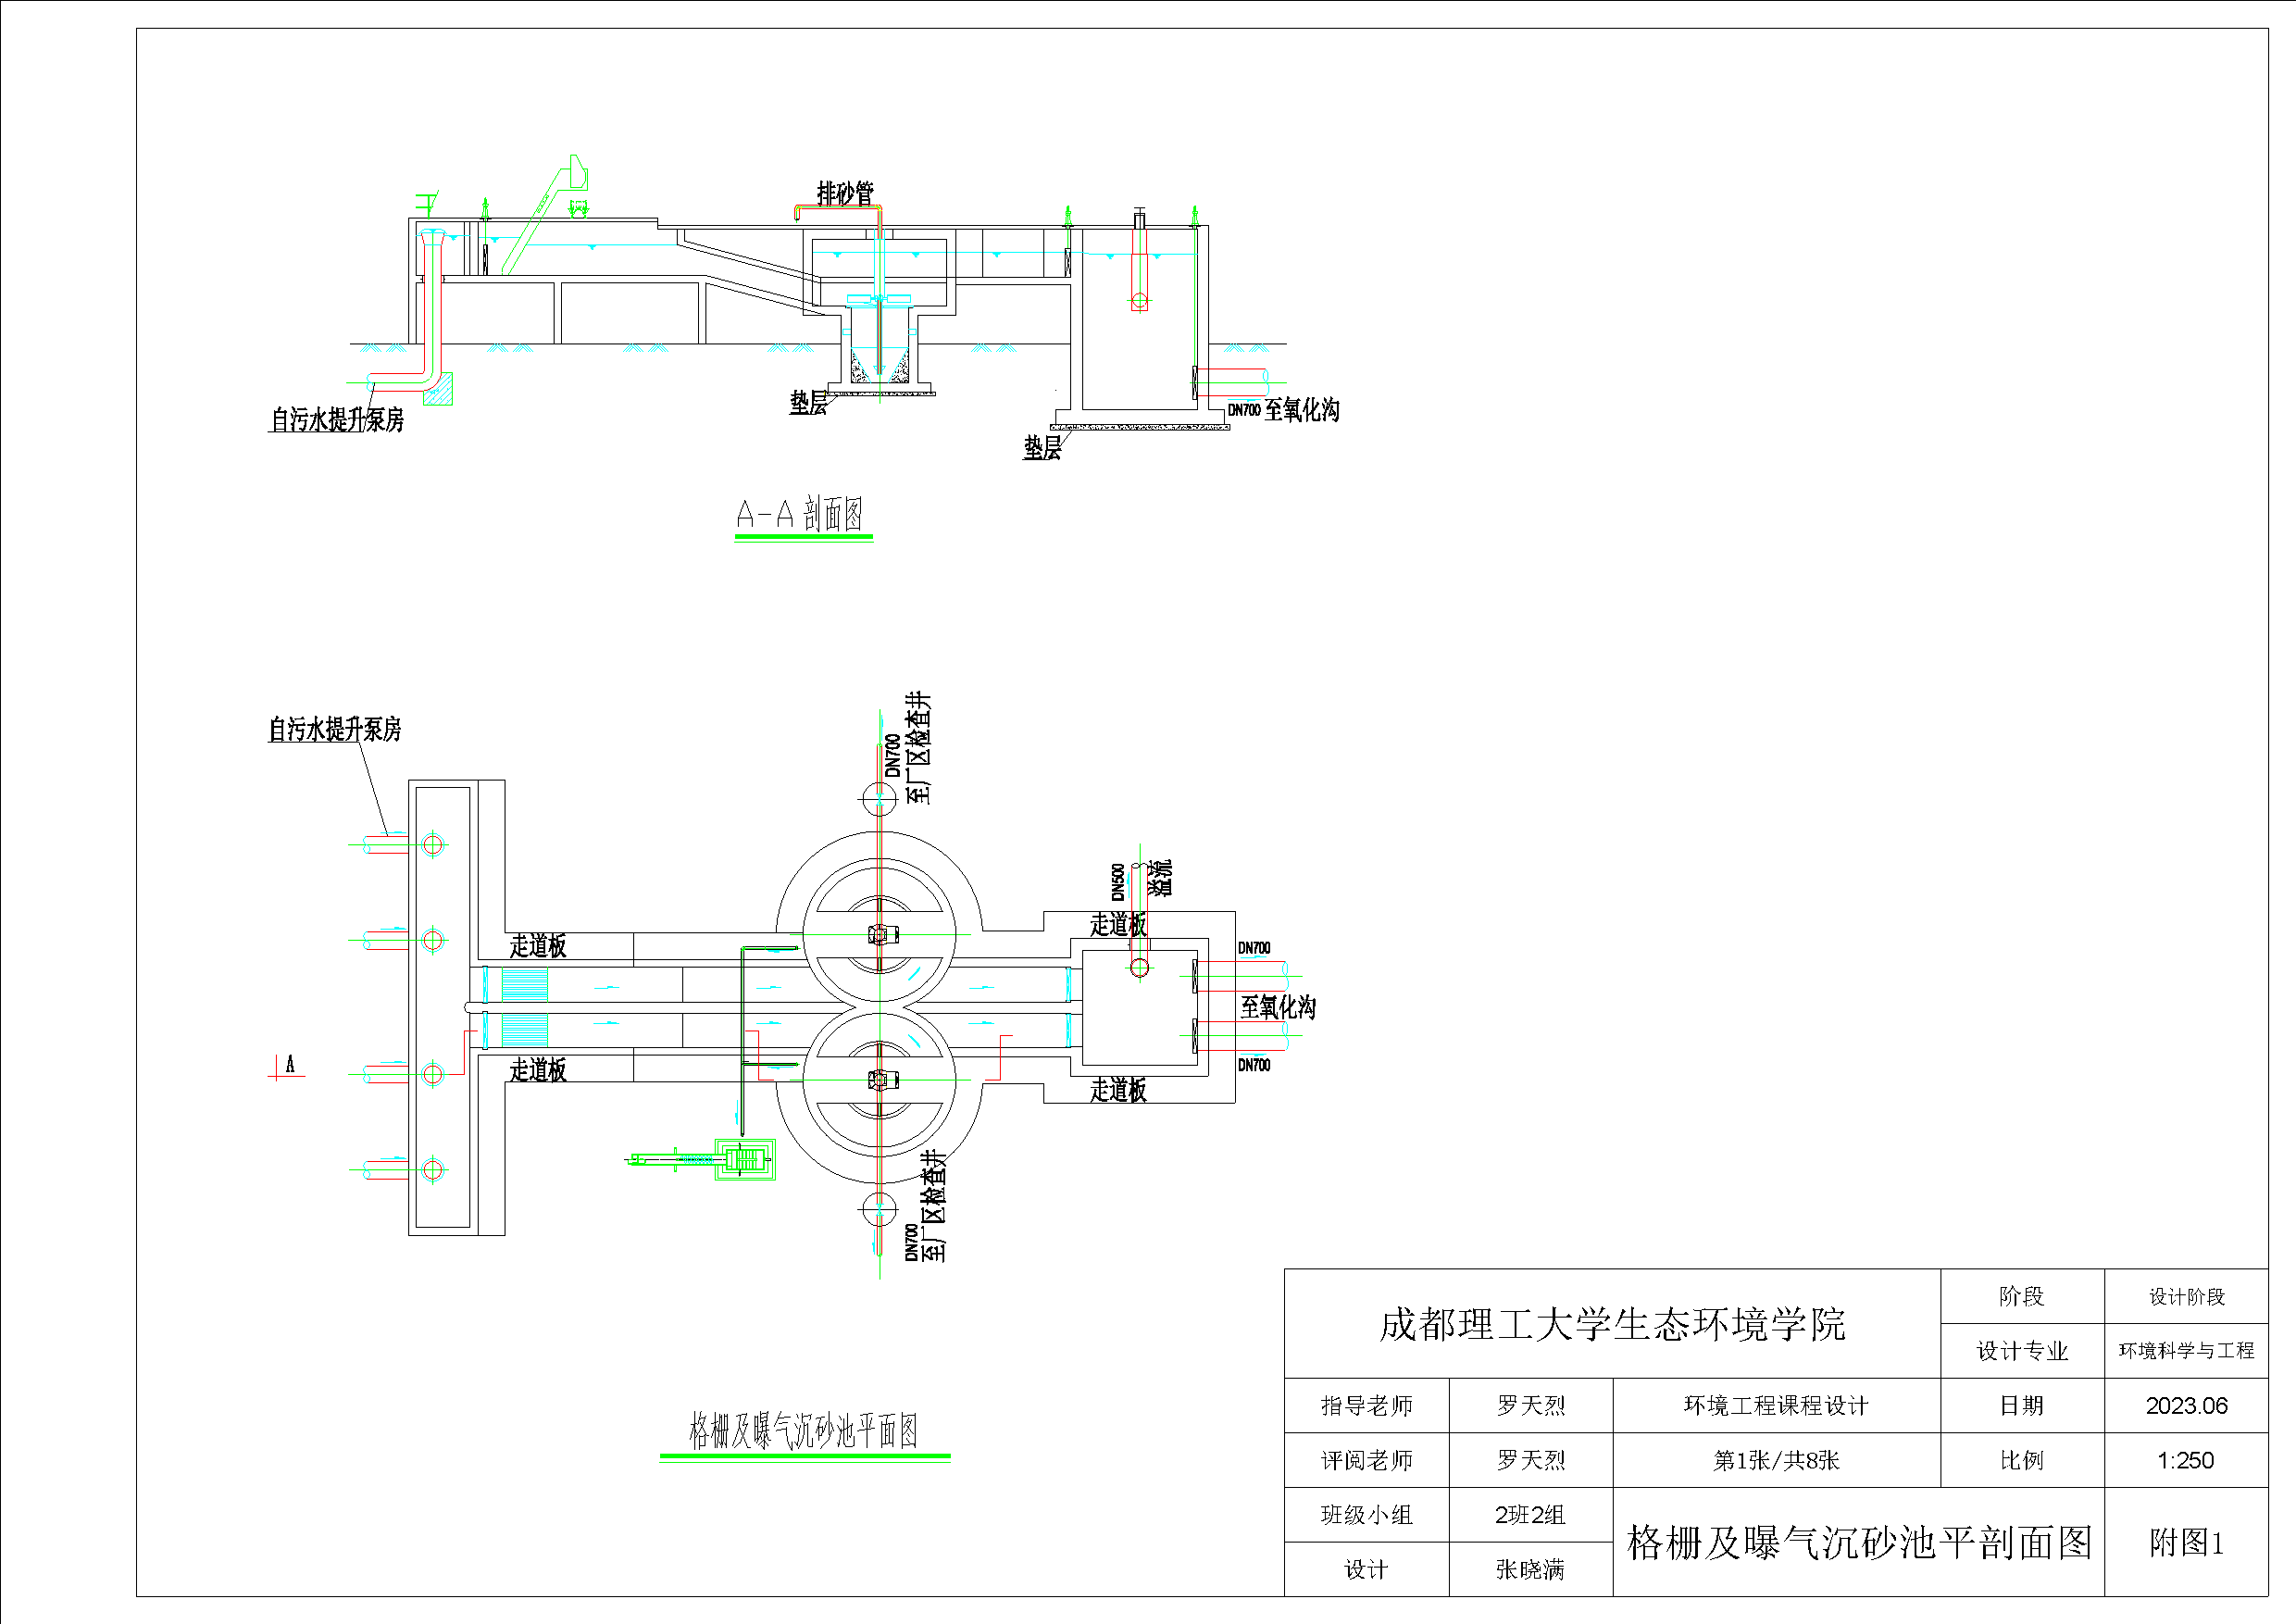
\includegraphics[width=1.15\textwidth]{drawing/Flat profile view of aeration grit tank.pdf}}
\end{figure}

\thumbnail{改良卡鲁塞尔氧化沟平剖面}
\begin{figure}[H]
	\centering
	\rotatebox{90}{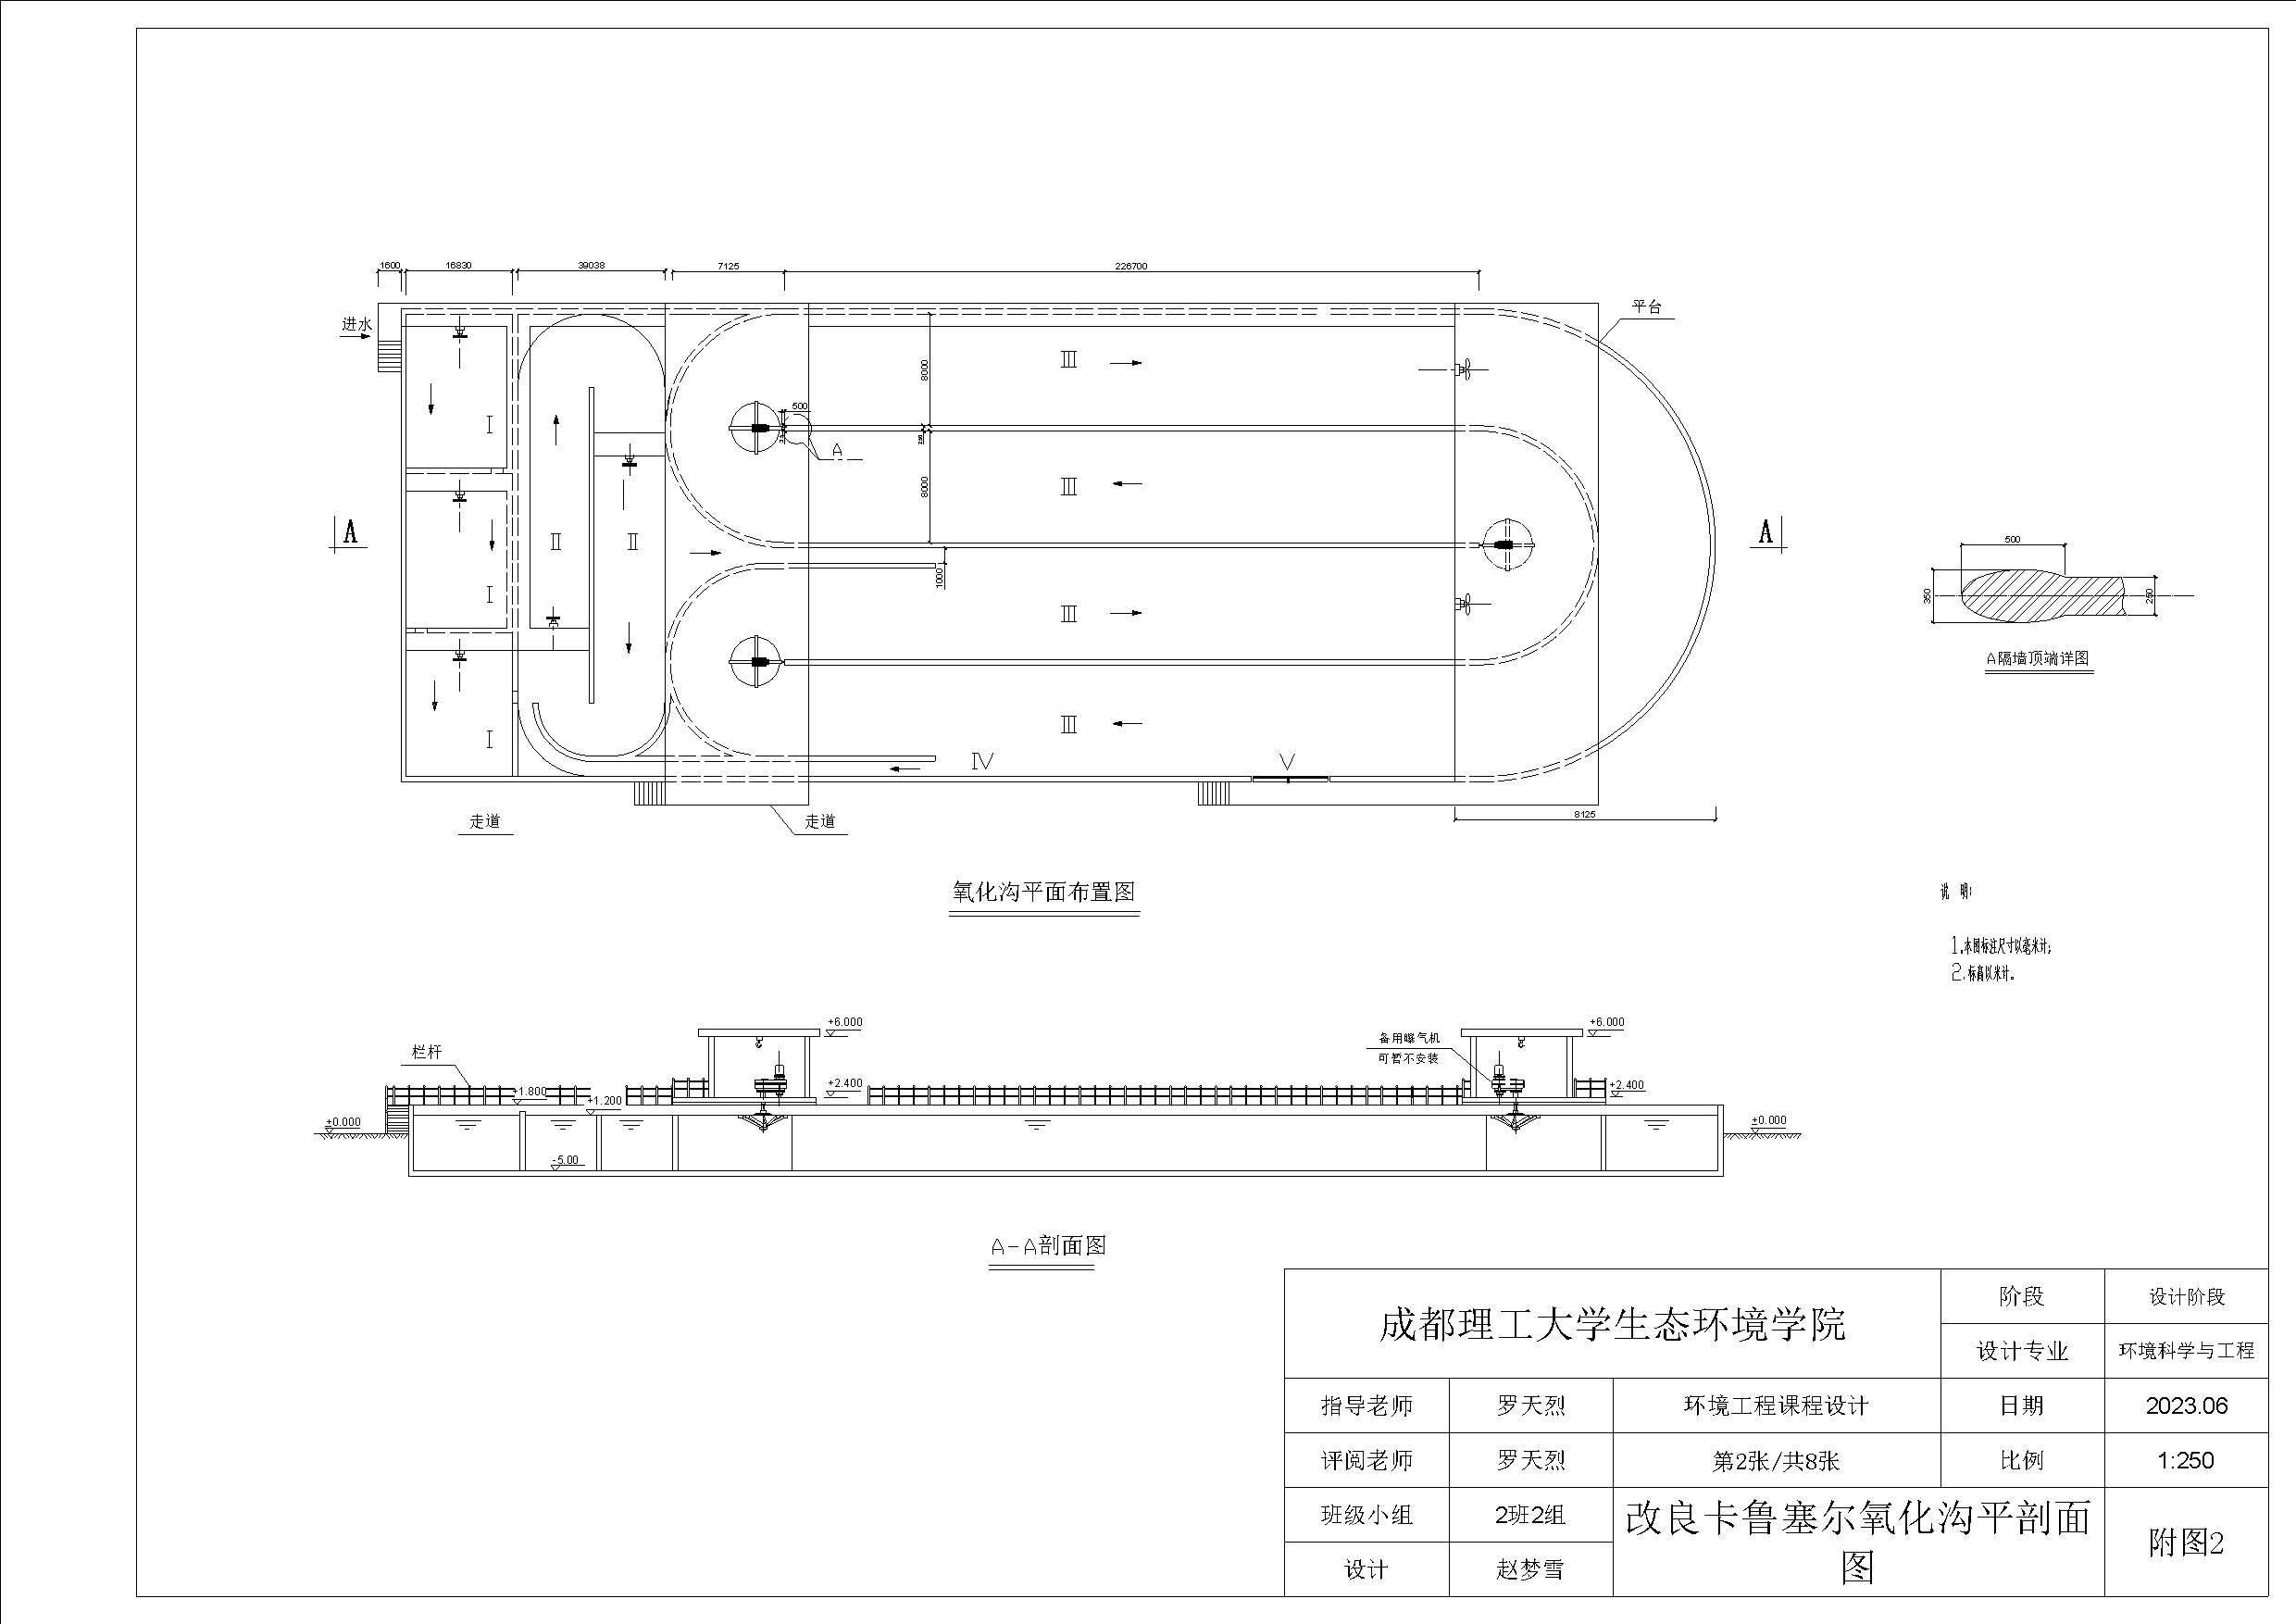
\includegraphics[width=1.15\textwidth]{drawing/Modified Carrousel oxidation groove flat profile.pdf}}
\end{figure}

\thumbnail{二沉池平剖面图}
\begin{figure}[H]
	\centering
	\rotatebox{90}{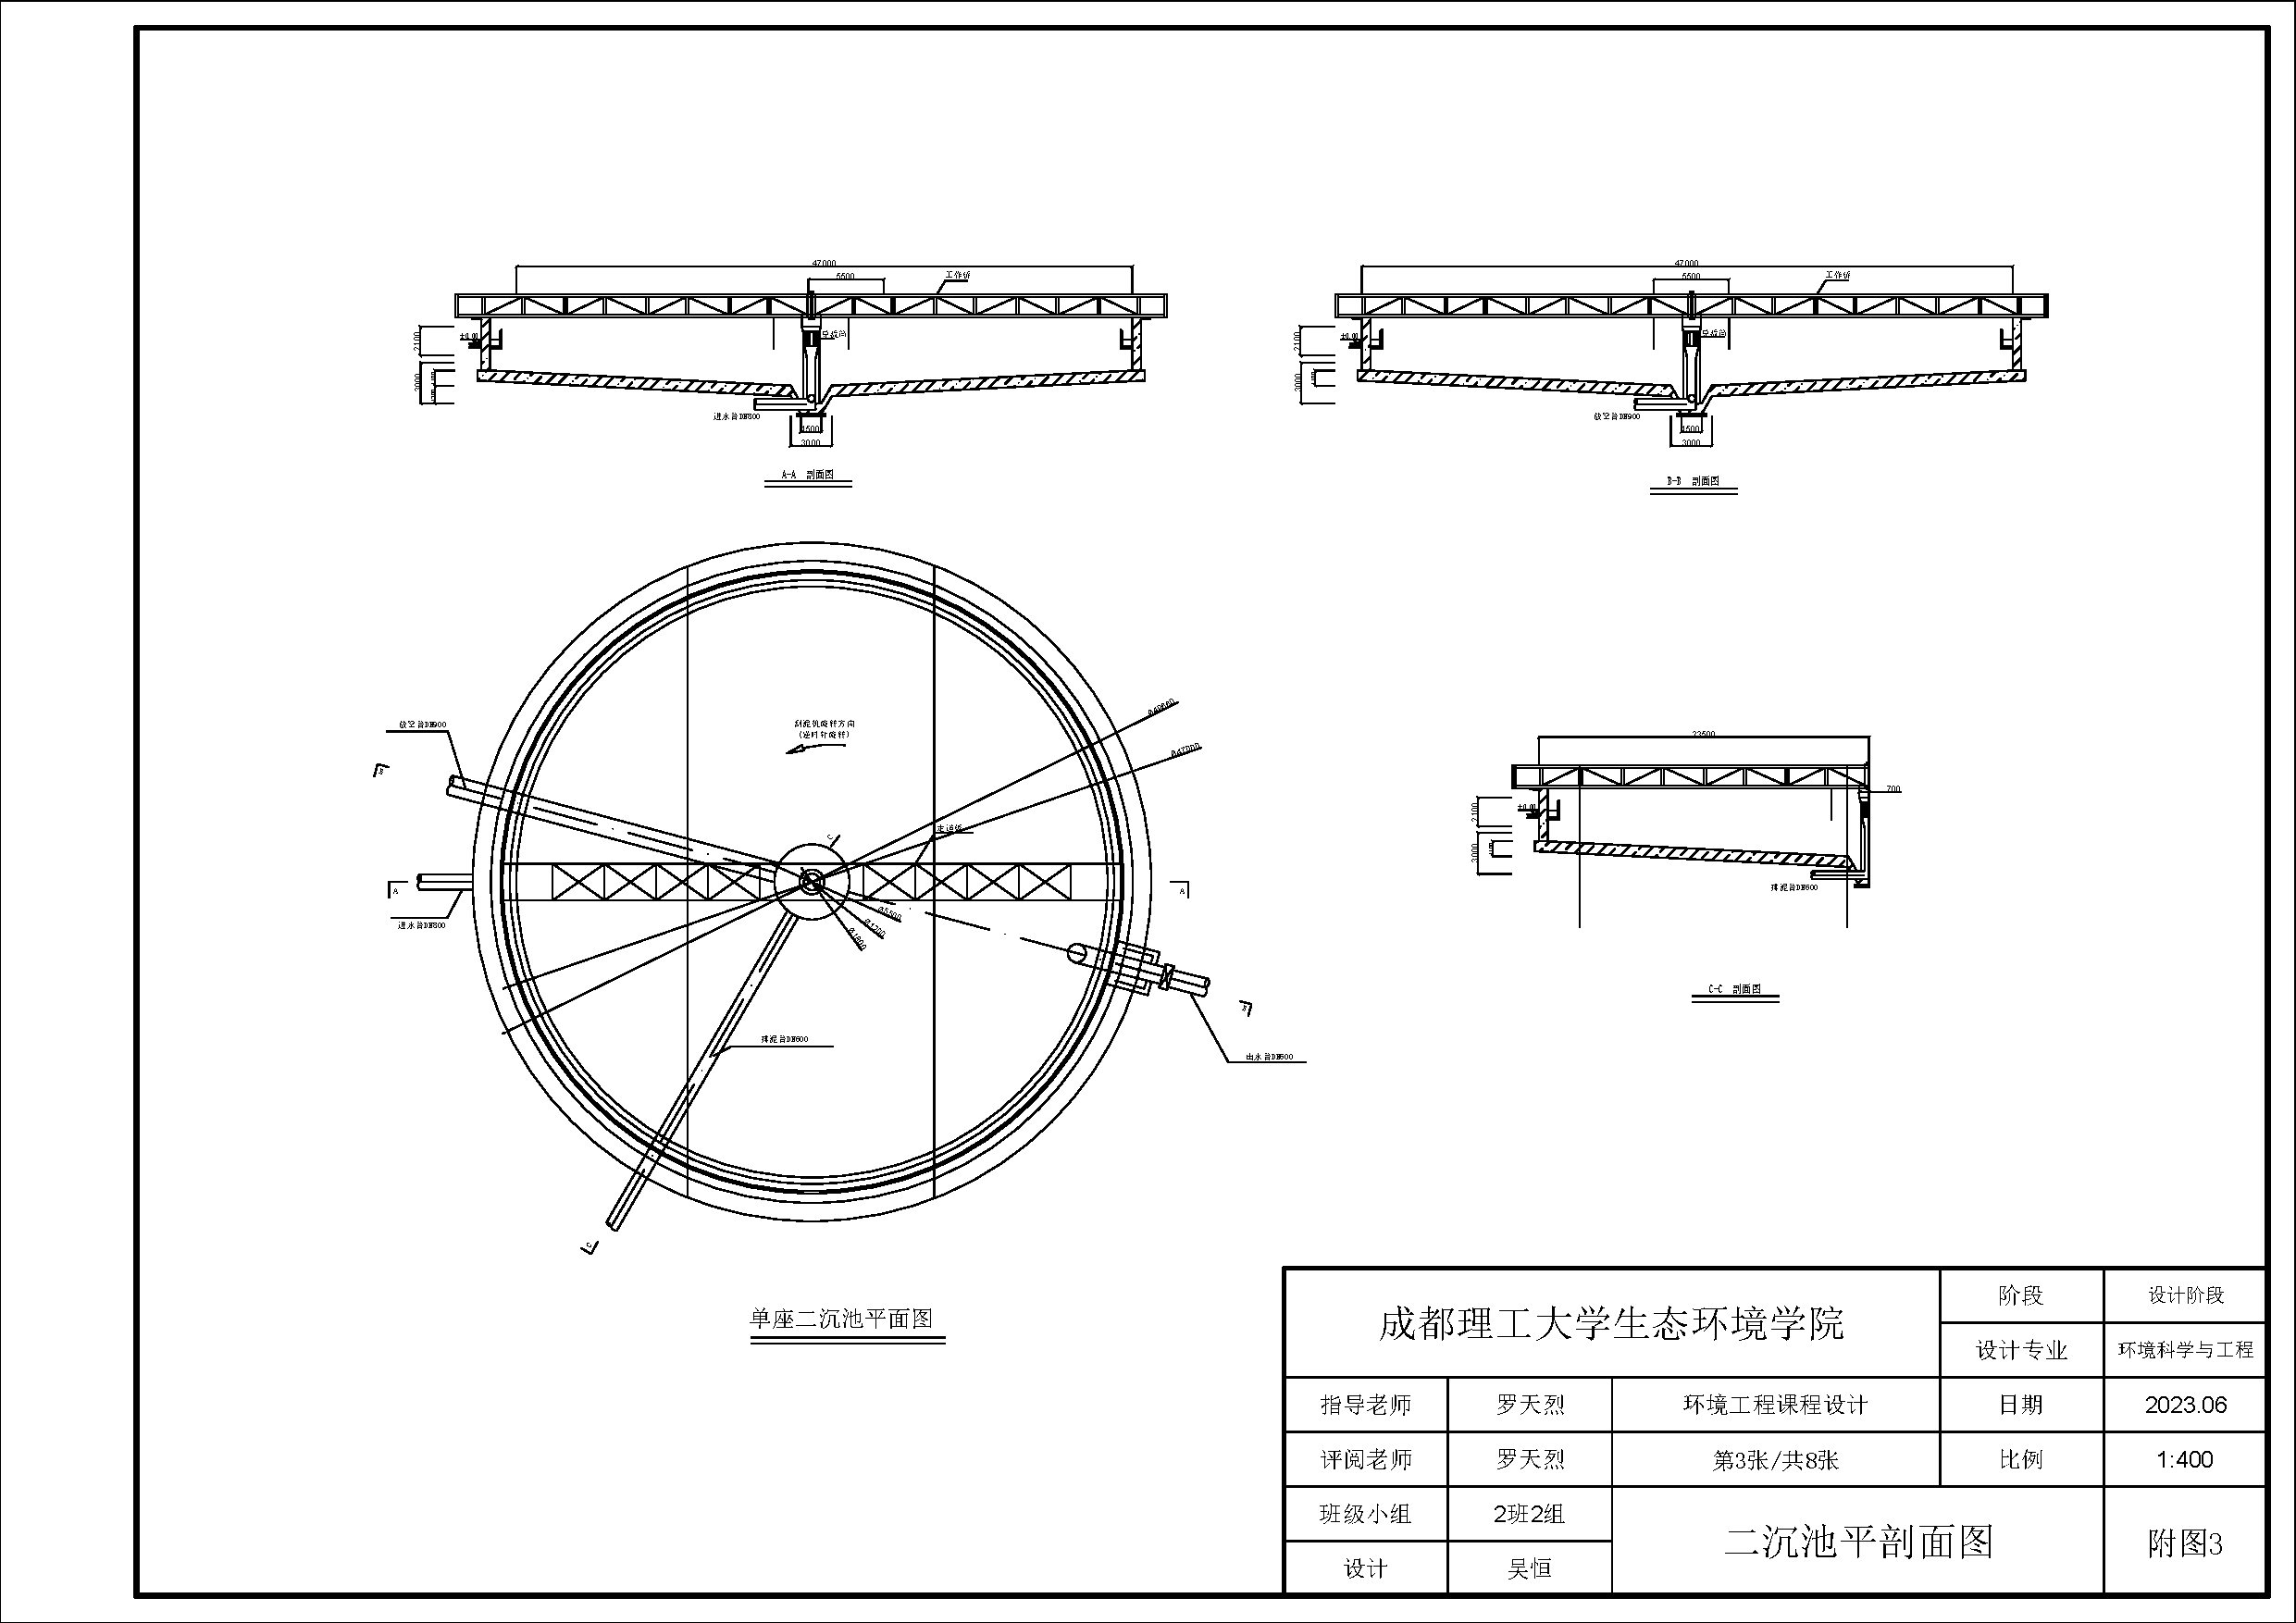
\includegraphics[width=1.15\textwidth]{drawing/2. Flat profile view of the sedimentation tank.pdf}}
\end{figure}

\thumbnail{加压溶气气浮池}
\begin{figure}[H]
	\centering
	\rotatebox{90}{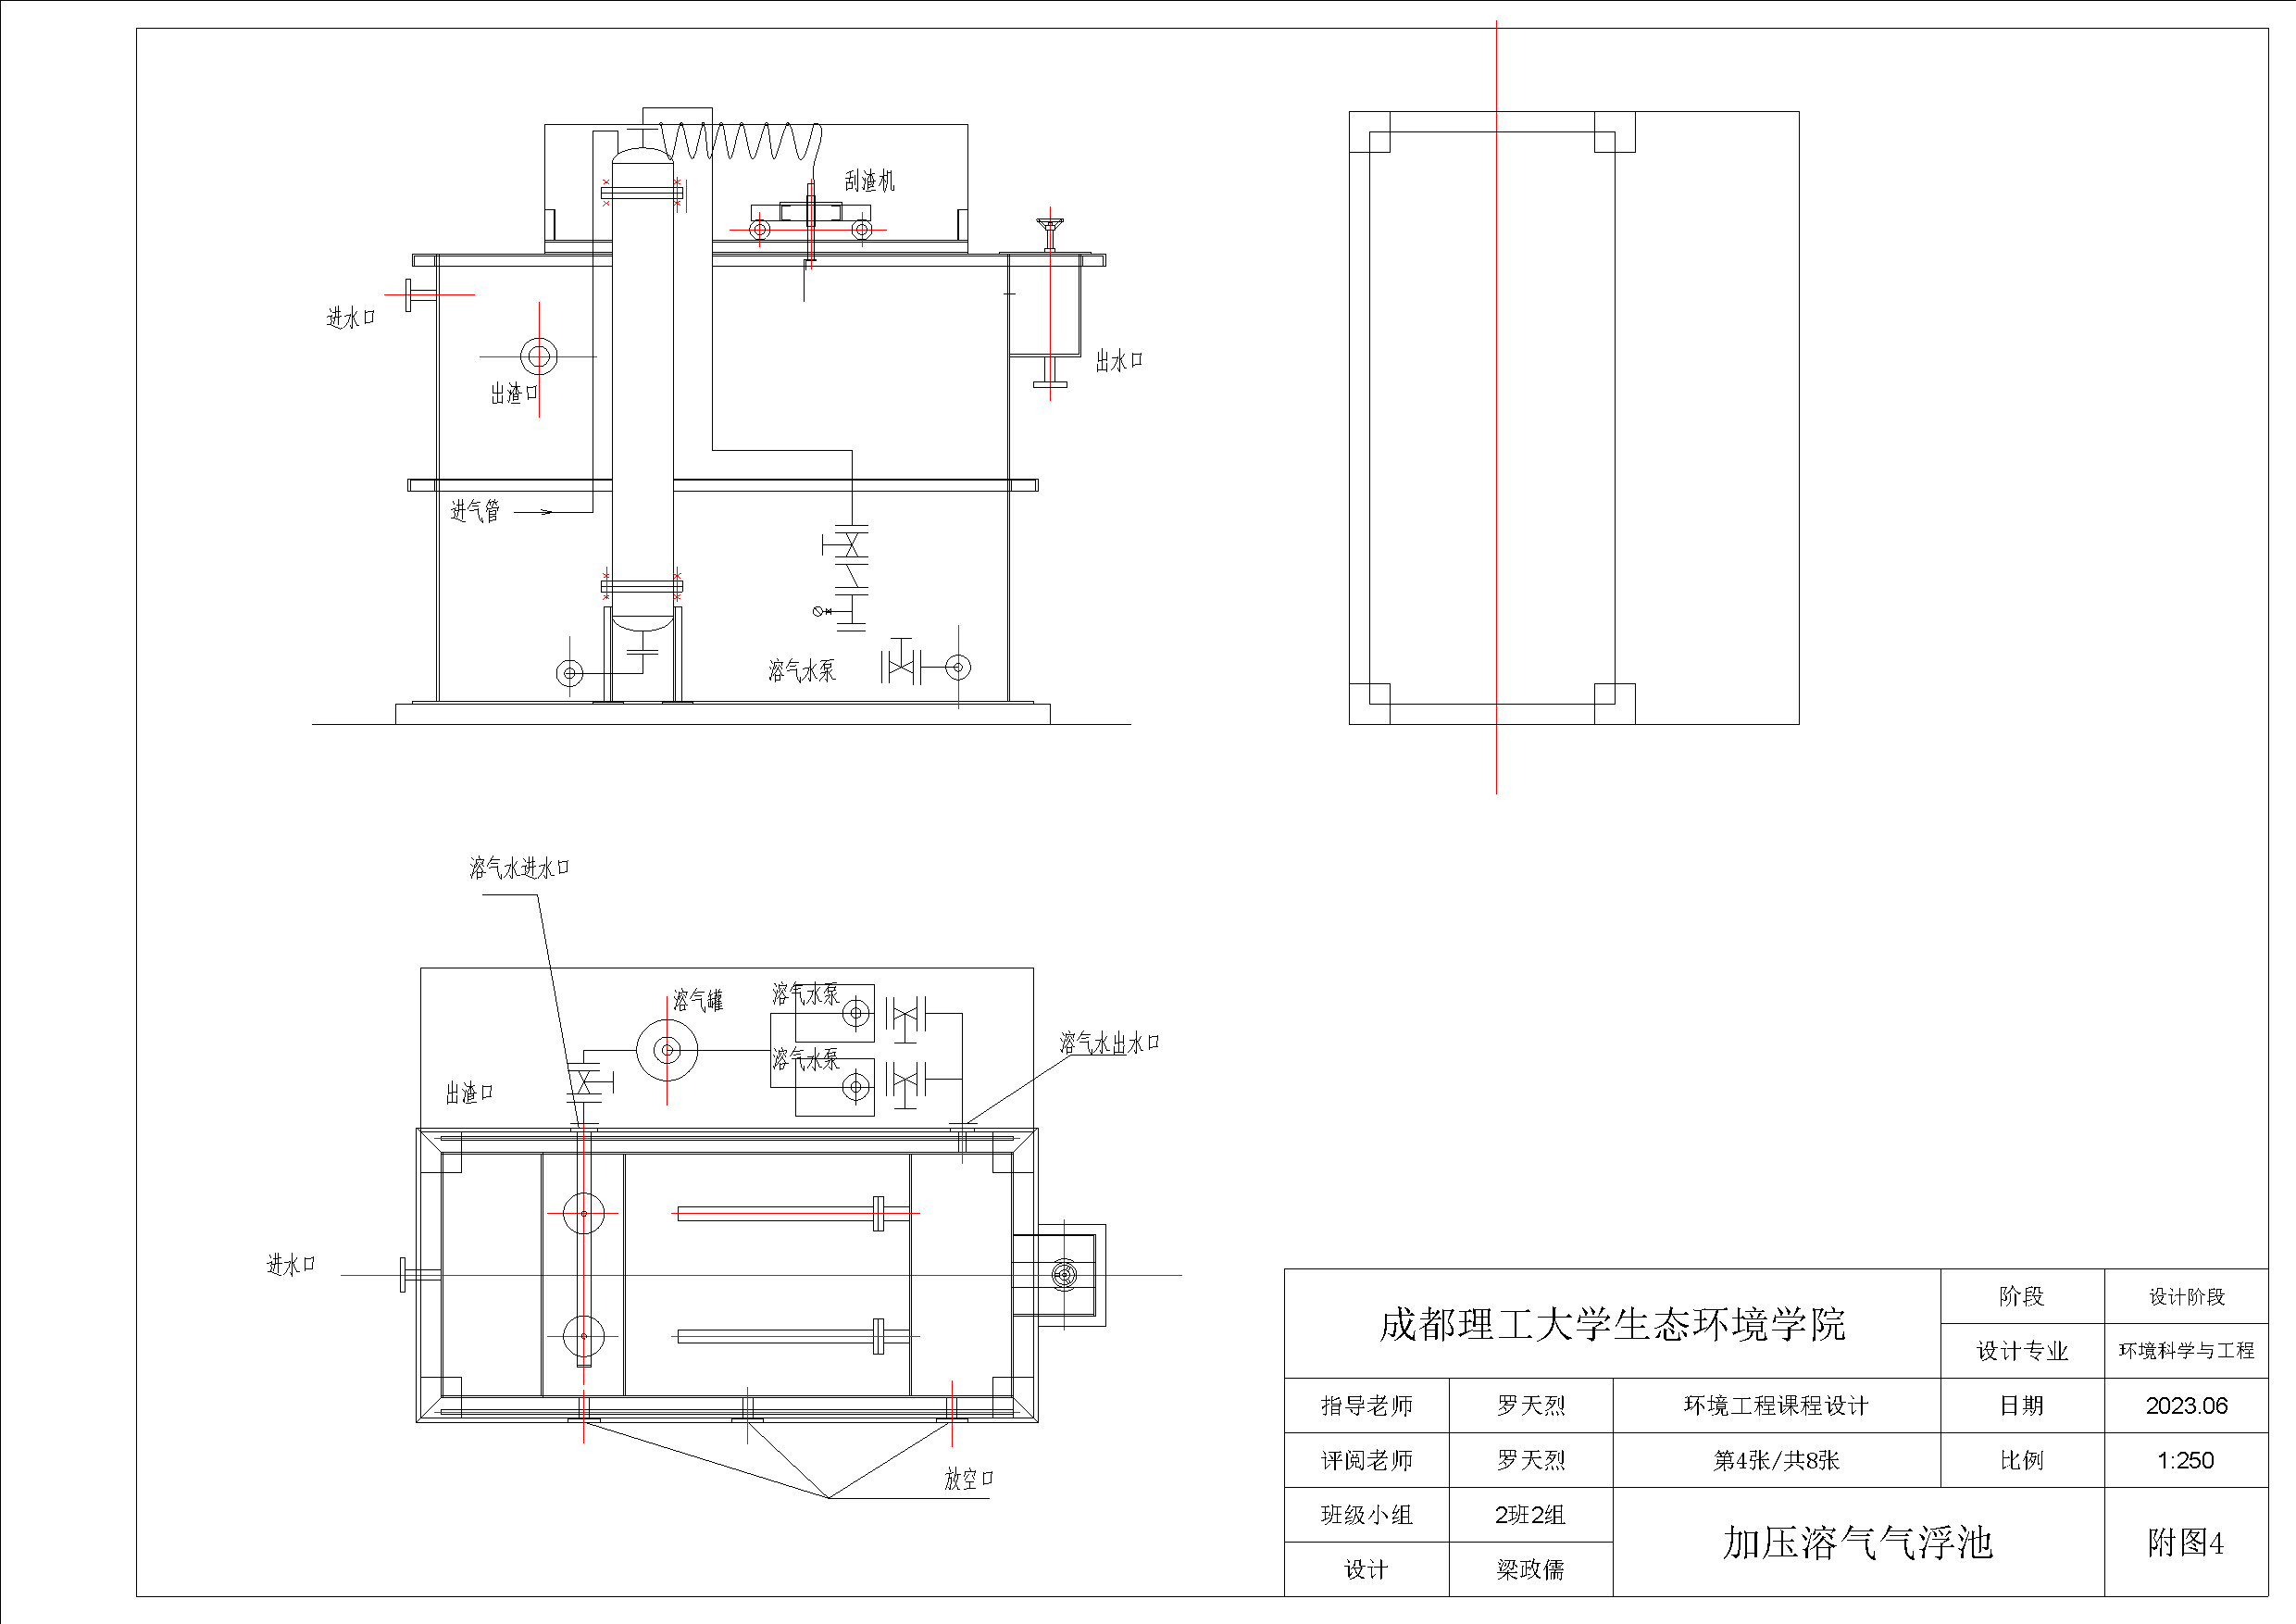
\includegraphics[width=1.15\textwidth]{drawing/Flat section of a pressurized air flotation tank.pdf}}
\end{figure}

\thumbnail{臭氧消毒池平剖面图}
\begin{figure}[H]
	\centering
	\rotatebox{90}{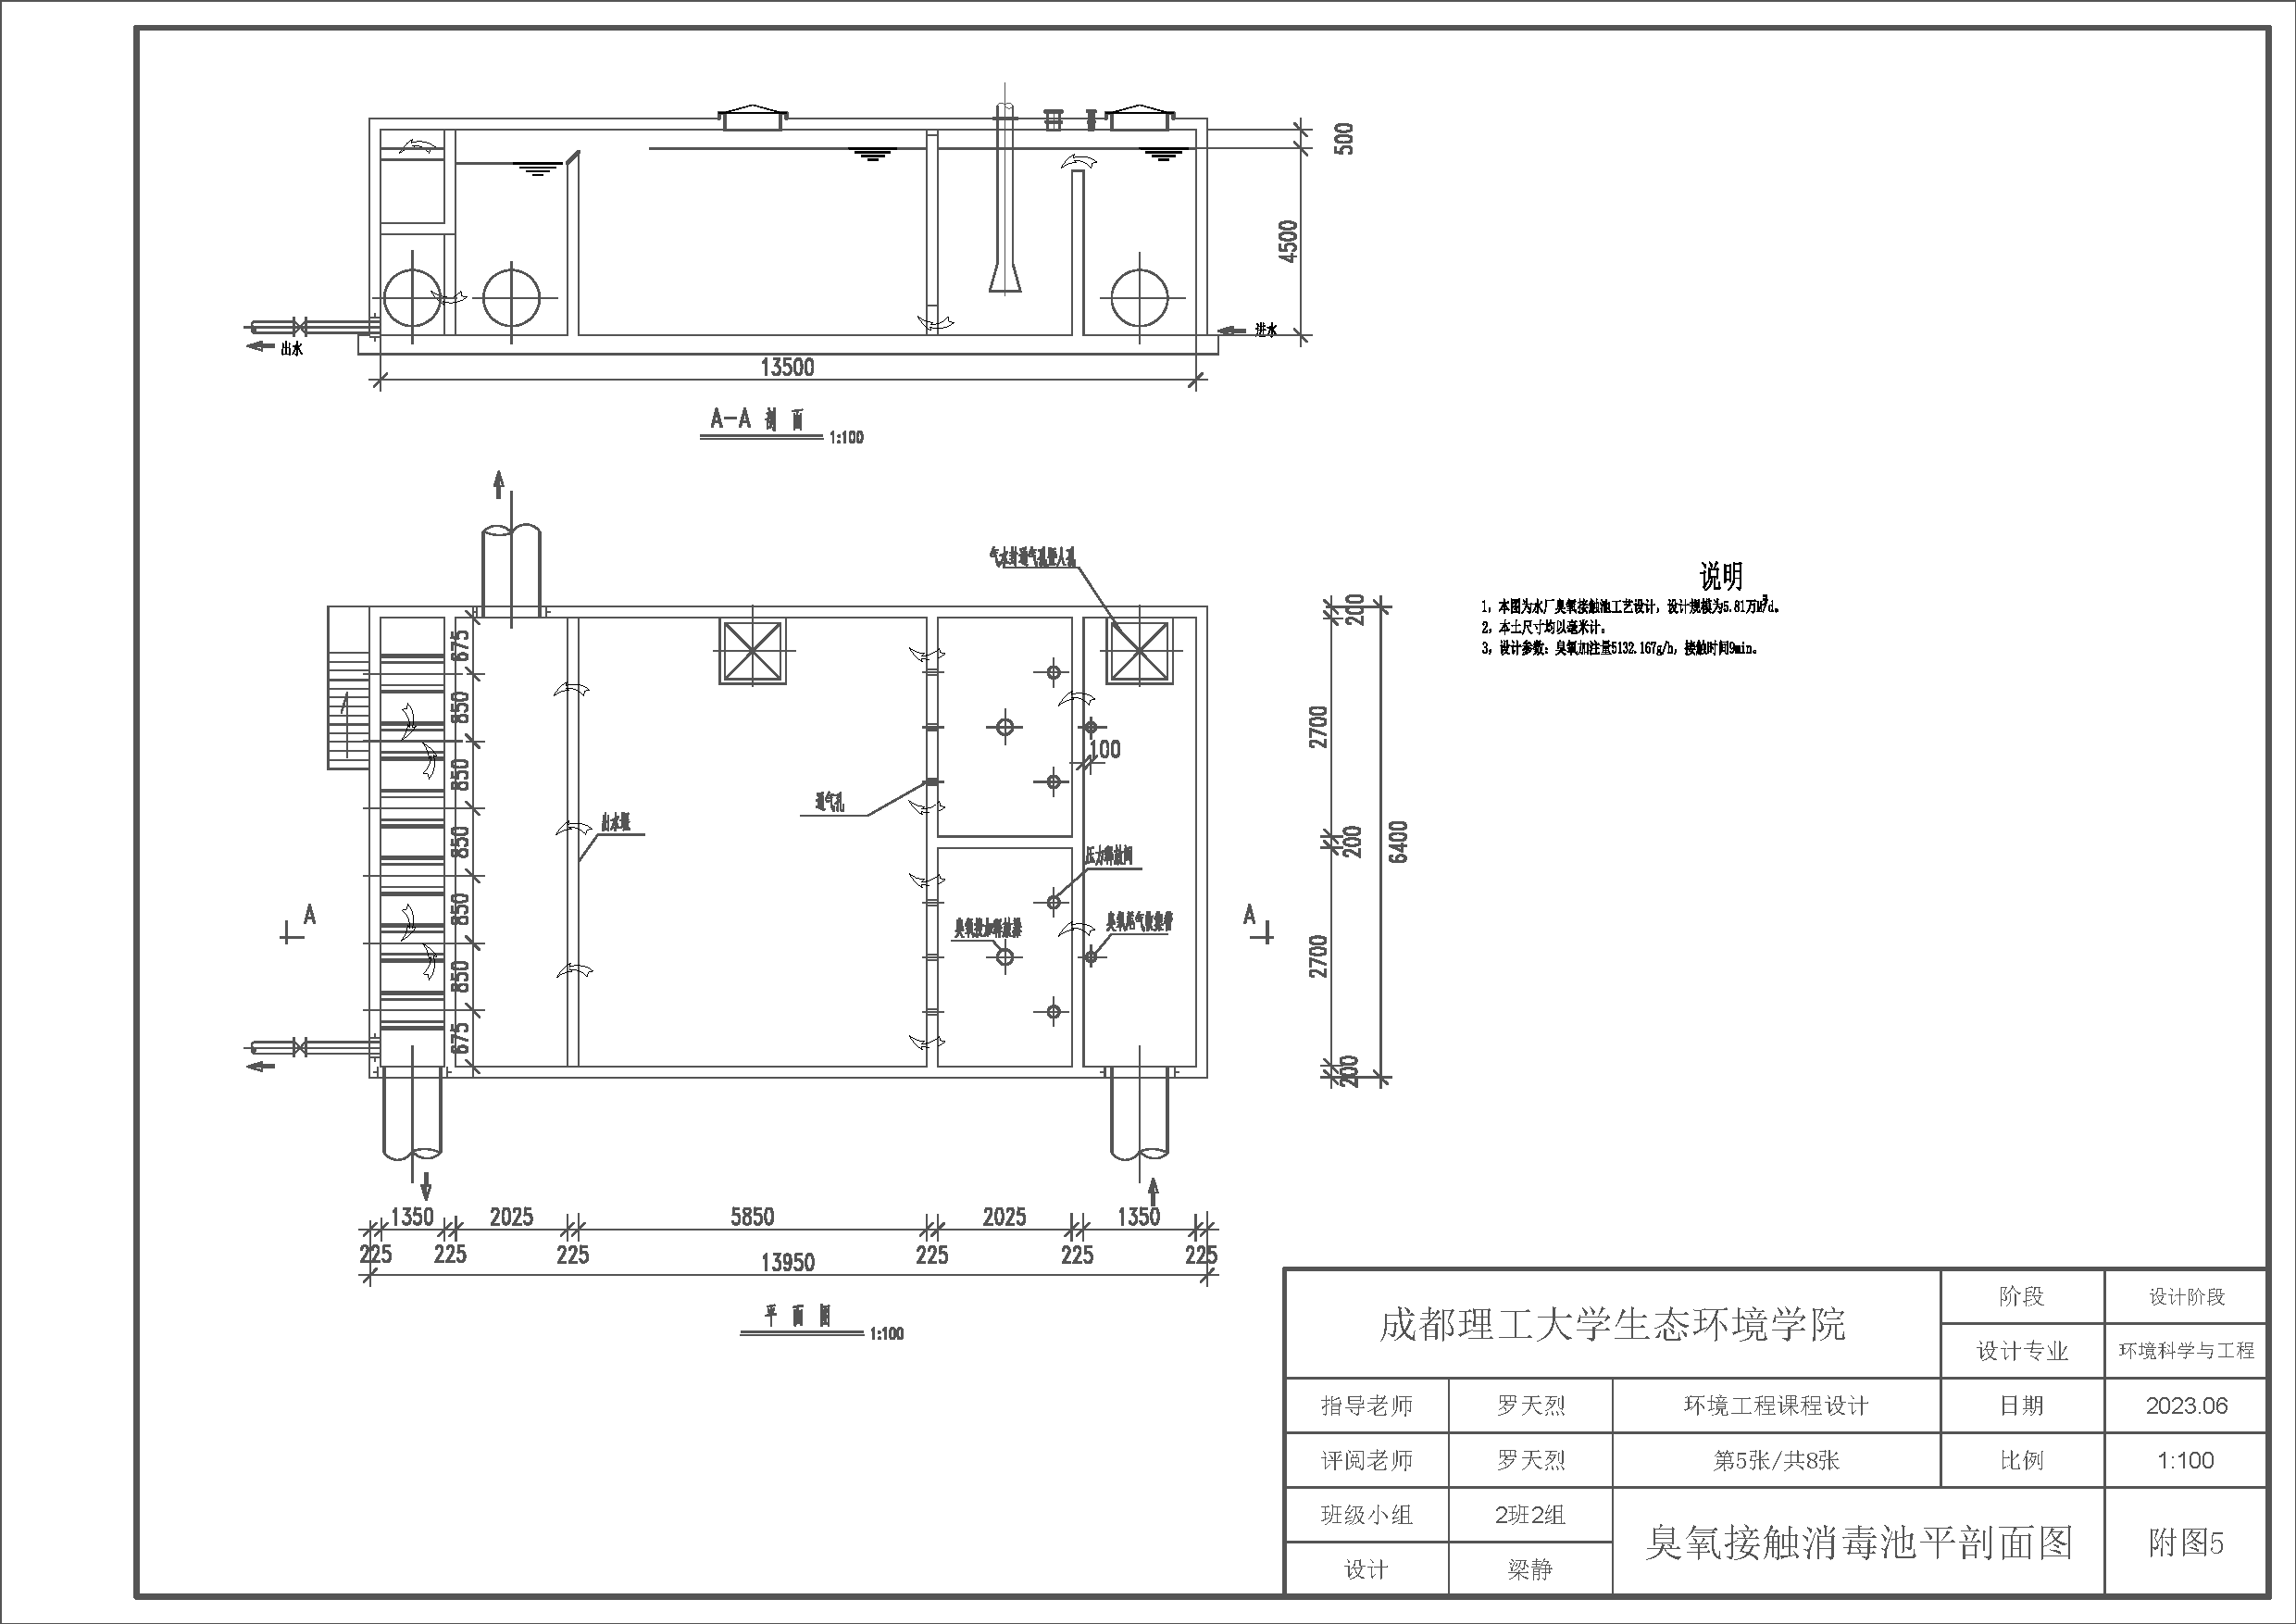
\includegraphics[width=1.15\textwidth]{drawing/Flat profile view of ozone disinfection tank.pdf}}
\end{figure}

\thumbnail{提升泵房平剖面图}
\begin{figure}[H]
	\centering
	\rotatebox{90}{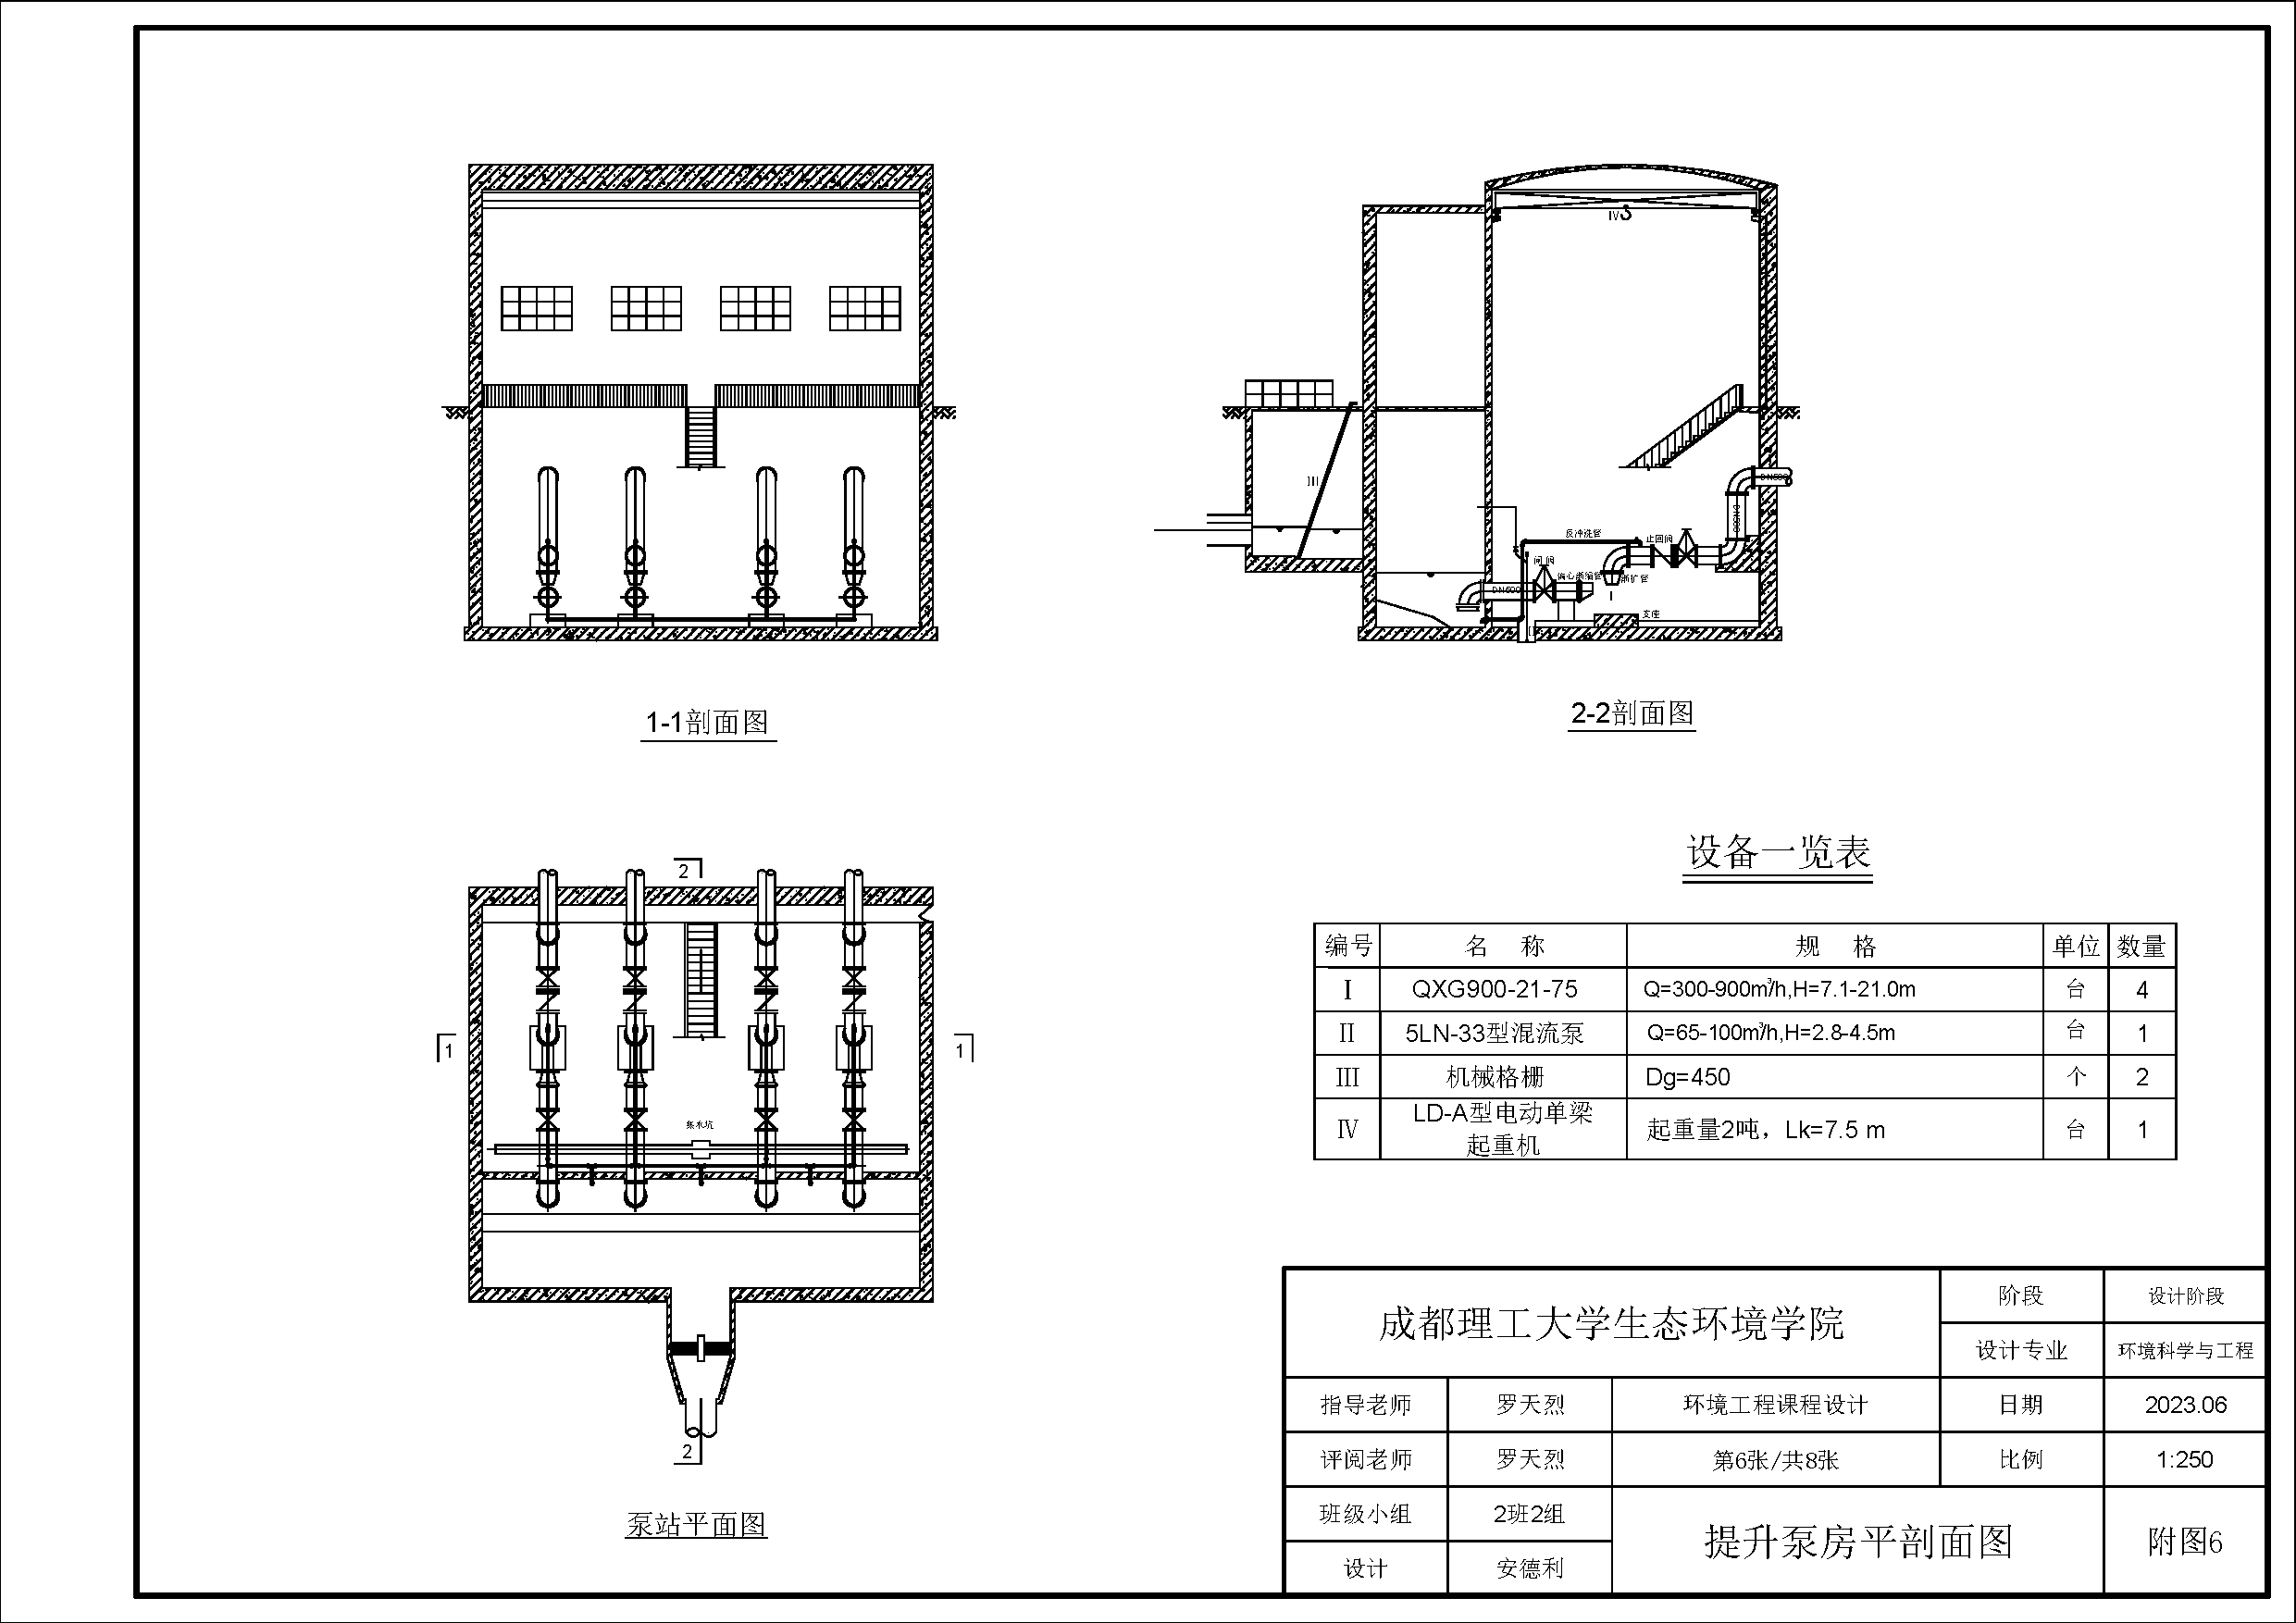
\includegraphics[width=1.15\textwidth]{drawing/Flat profile view of the lifting pump room.pdf}}
\end{figure}

\thumbnail{污水处理厂平面布置图}
\begin{figure}[H]
	\centering
	\rotatebox{90}{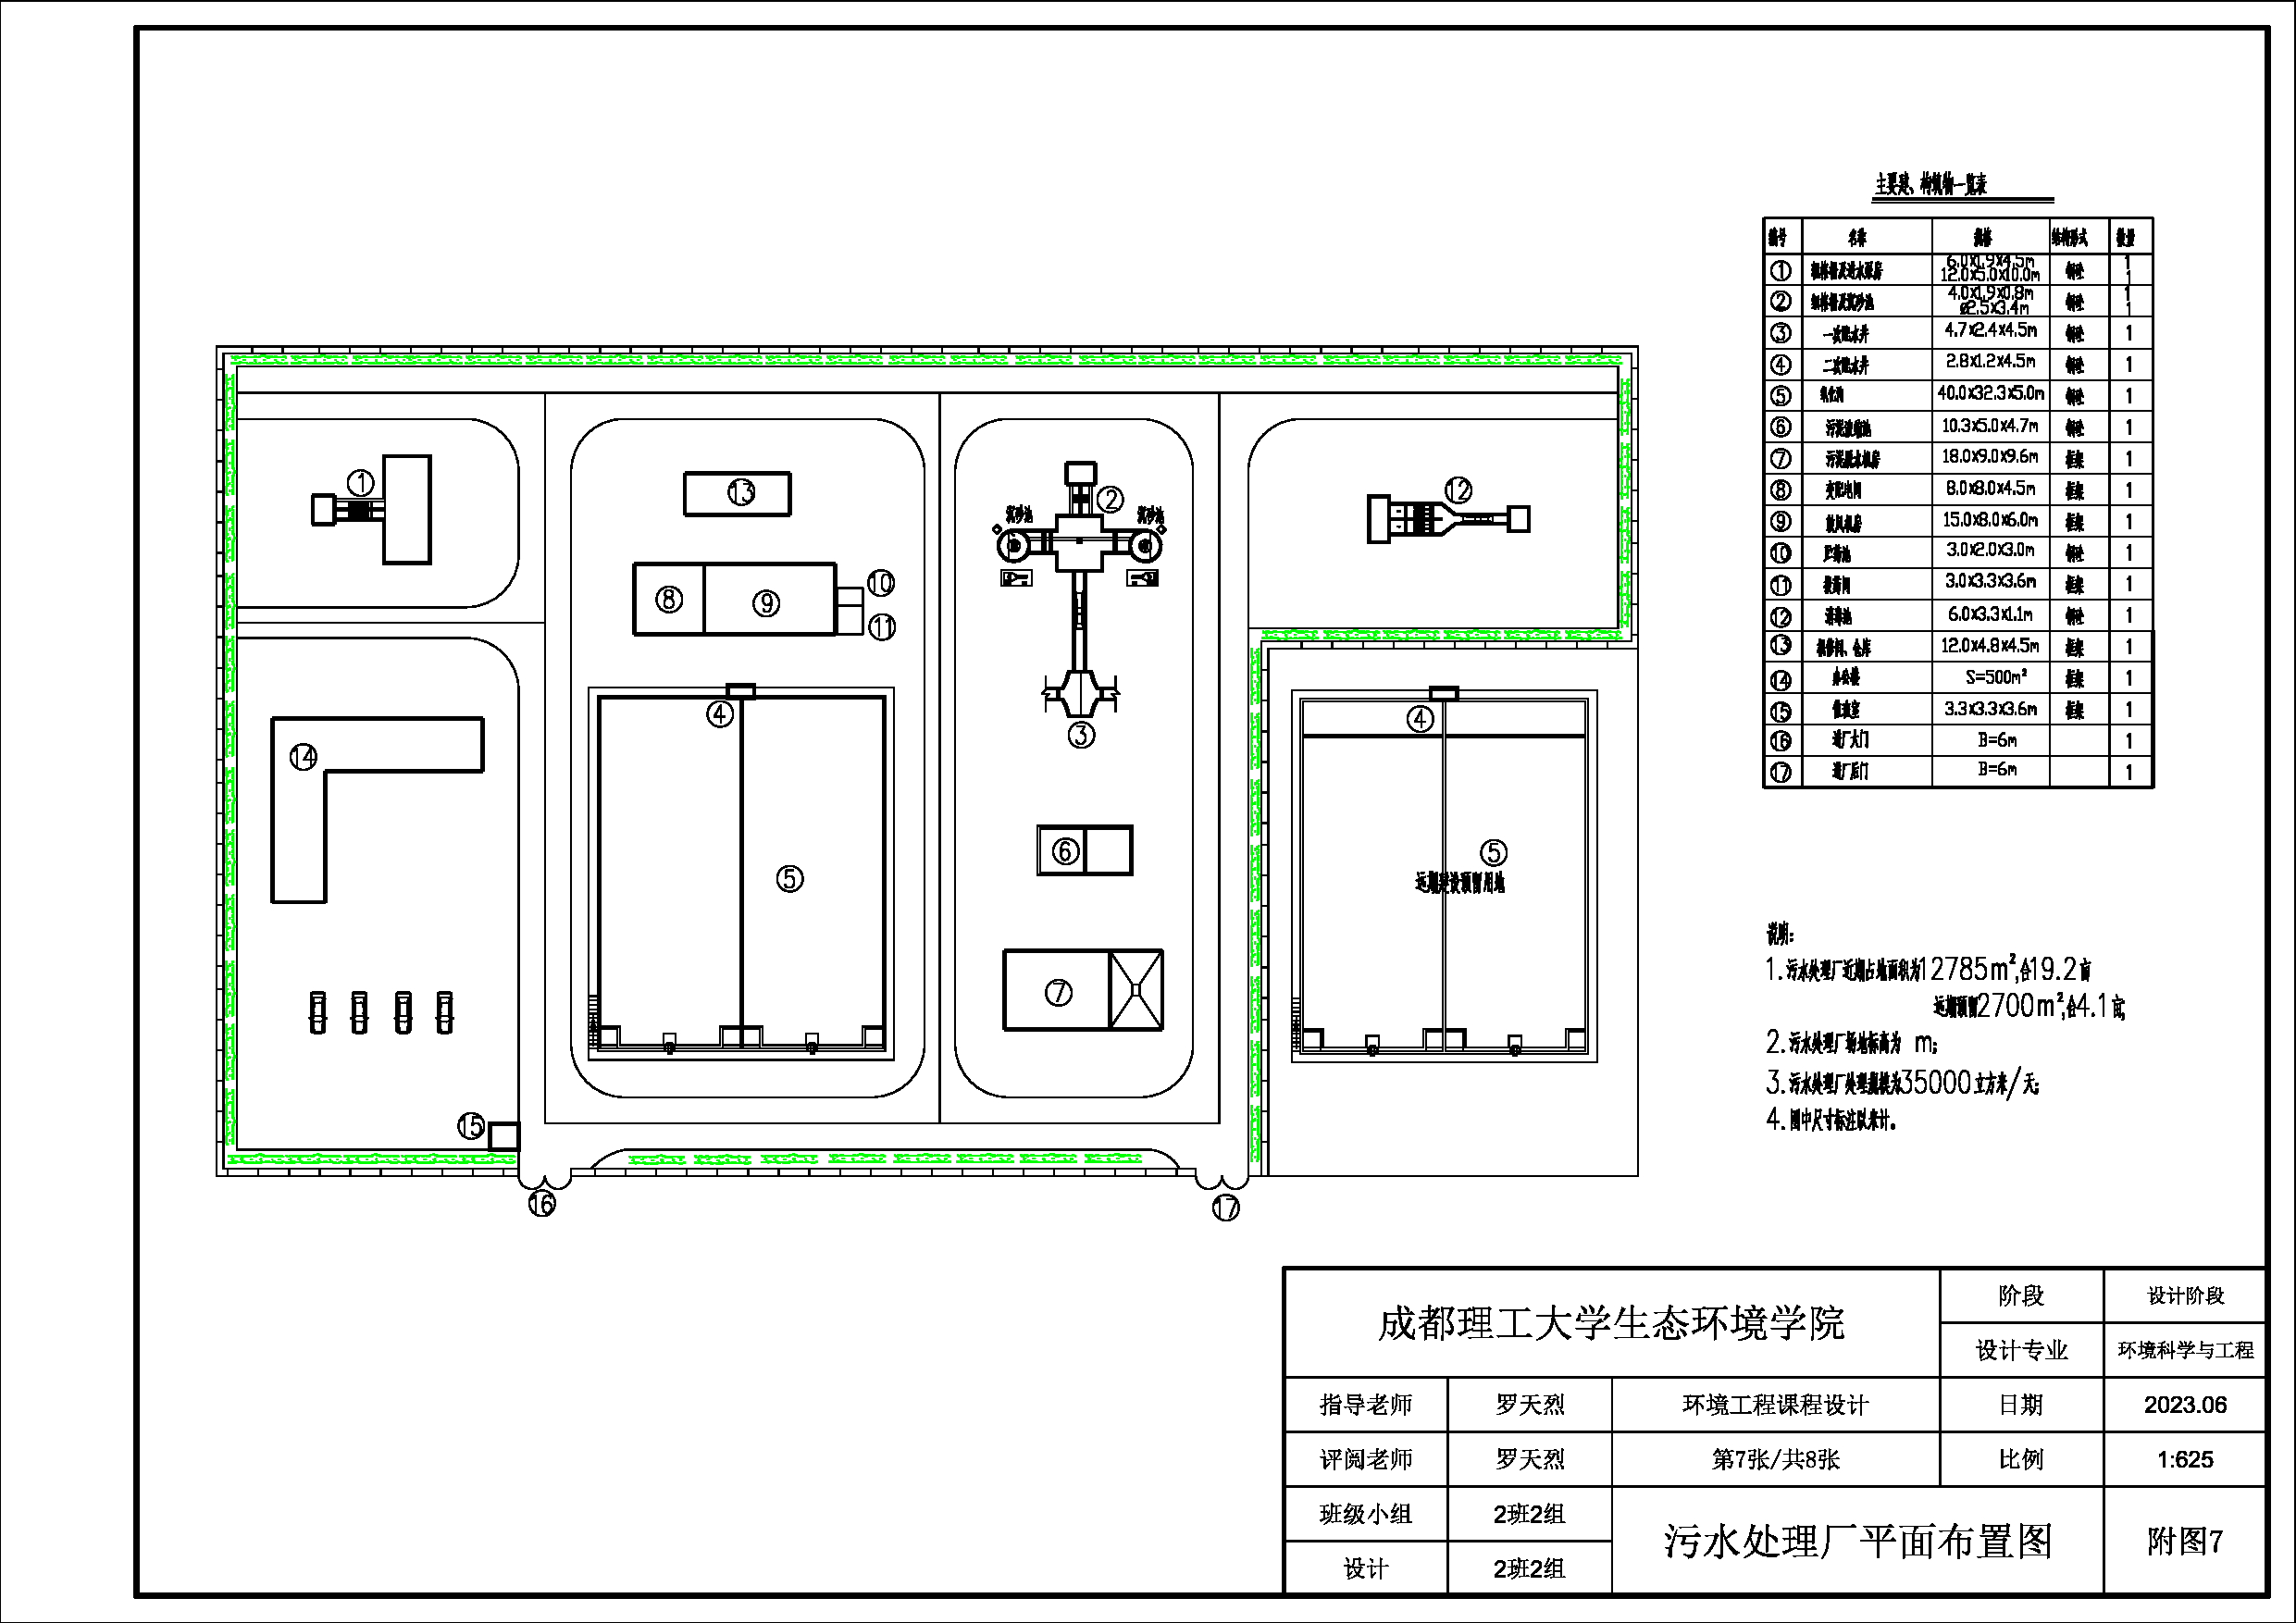
\includegraphics[width=1.15\textwidth]{drawing/Floor plan of the sewage treatment plant.pdf}}
\end{figure}

\thumbnail{污水处理厂高程布置图}
\begin{figure}[H]
	\centering
	\rotatebox{90}{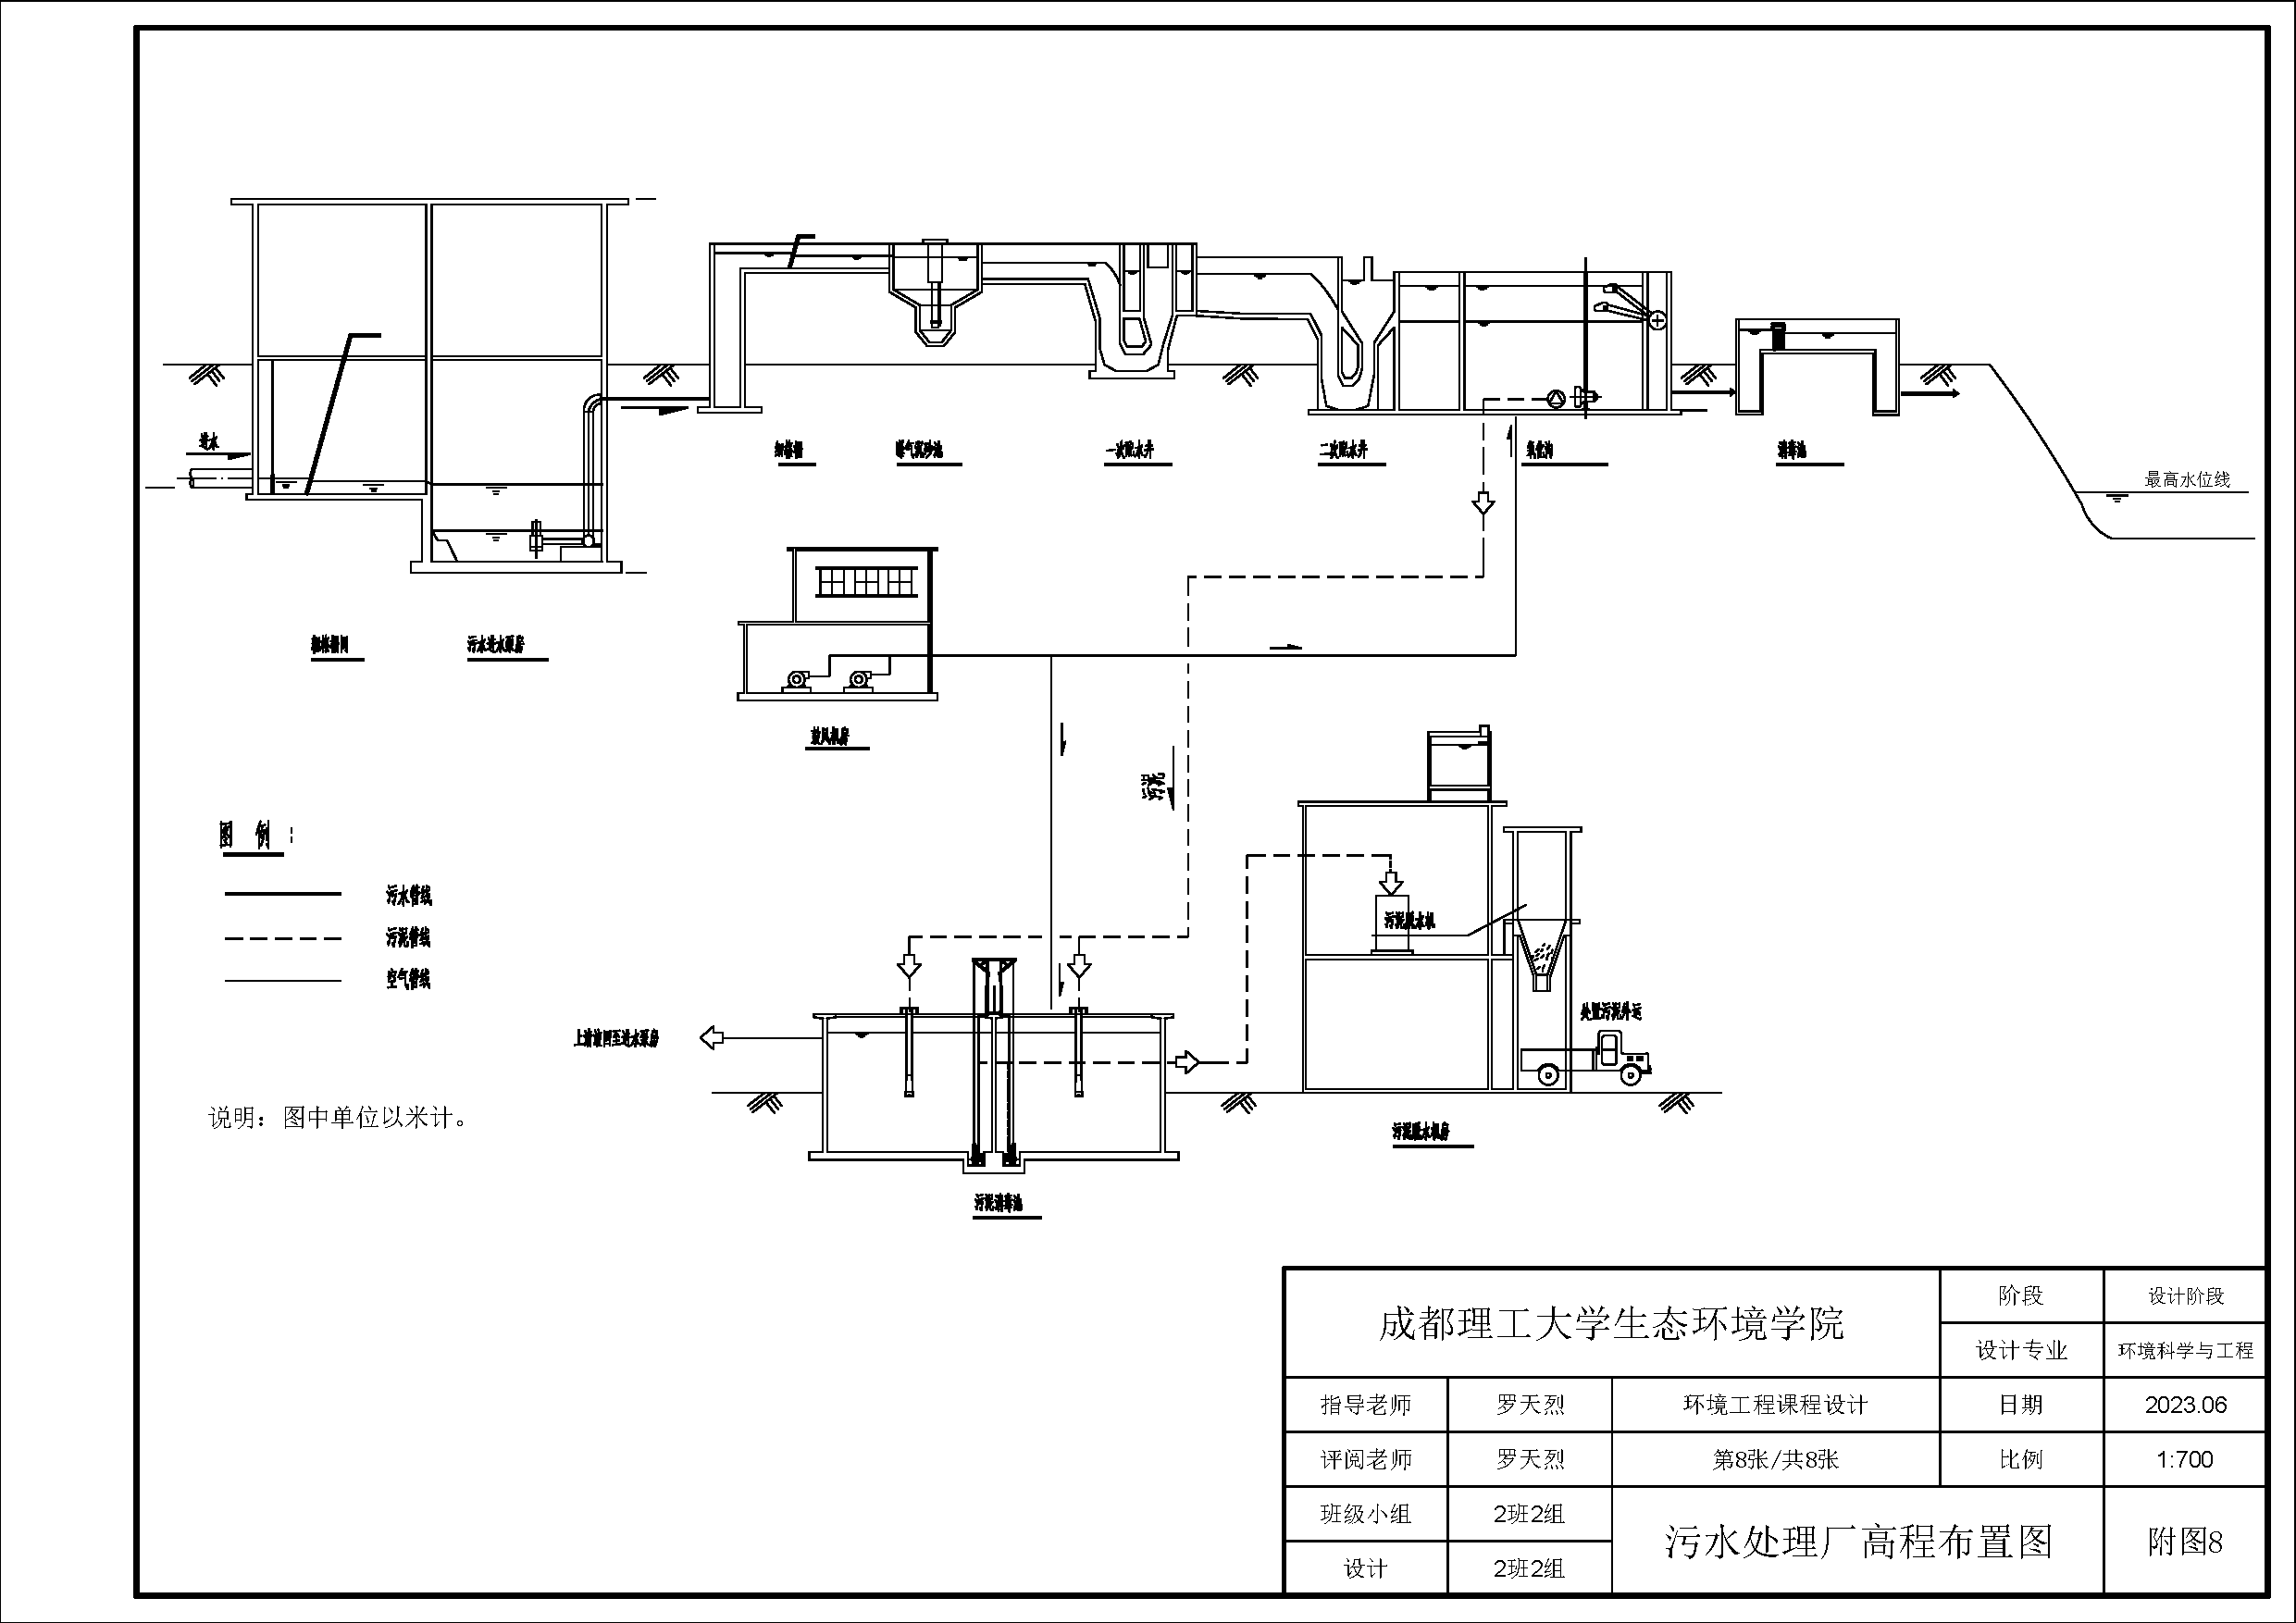
\includegraphics[width=1.15\textwidth]{drawing/Elevation layout of a sewage treatment plant.pdf}}
\end{figure}

 % CAD图纸

\end{document}